\documentclass{article}
\usepackage[utf8]{inputenc}
\usepackage{amsfonts}
\usepackage{geometry}
\usepackage{amsmath}
\usepackage{todonotes}
\usepackage{amsthm}
\usepackage{hyperref}
\usepackage{physics}
\usepackage{graphicx}
\usepackage{subcaption}
% \usepackage[square,sort,comma,numbers]{natbib}

\newtheorem{theorem}{Theorem}

\newcommand{\ob}[1]{\textcolor{blue}{\bf [[[Ollie: #1]]]}}
\newcommand{\mce}[1]{\textcolor{purple}{[Matt: #1]}}
\newcommand{\pmr}[1]{\textcolor{purple}{[Patricio: #1]}}
\newcommand{\avi}[1]{\textcolor{red}{[Avi: #1]}}

\geometry{a4paper, top=1cm, bottom=3cm, left=1.5cm, right=3.5cm,heightrounded,bindingoffset=5mm }

\title{Wavelets}
\author{ Q.~Baghi, O.~Burke, G.~Mentasti, A.~Vajpeyi}
\date{May 12, 2023}

\begin{document}

\maketitle

\tableofcontents


\section{Introduction}
Gravitational wave detector noise exhibits non-stationarity due to transient fluctuations, long-term spectral drifts, and data-stream gaps. 
These effects induce correlations across frequency samples, exacerbating the challenges of frequency domain analysis. 
One method to address this is to use a time-frequency data analysis approach, employing discrete wavelet wavepackets. 
Mapping time domain data onto a uniform grid of time-frequency pixels mitigates correlations, particularly for locally stationary noise. 
In this work, we introduce an open-source GPU-accelerated Python library for gravitational wave time-frequency data analysis, PyWavelet. 
We provide a suite of examples, demonstrating Bayesian analysis of GW signals using the time-frequency domain versus traditional methods, while accounting for non-stationary noise effects. Detailed mathematical derivations for the wavelet domain analysis are available in supplementary materials.


\section{Definitions}
We are given a data stream in time domain, consisting of a set of N samples of a \textbf{real} quantity $x$ at times $\{t_k\}_{k=0\dots N-1}$ in a total time of observation $T$
\begin{align}\label{st_definition}
x[k]=x(t_k)\qquad,\qquad k=\{0\dots N-1\}\;,
\end{align}
sampled uniformly with sampling interval $\Delta t = t_{k+1} - t_{k}$ with $T = N\Delta t$. All of the information we have lies in these N points. We define the time sampling rate and the Nyquist frequency as
\begin{align}
r_s&\equiv\frac{1}{\Delta t}\equiv\frac{N}{T}\;,\nonumber\\
f_{\rm max}&=\frac 1 2r_s\;,\nonumber\\
\Delta f \equiv 1/(2\Delta t)
\end{align}
With that respect, if we set $t_0=0$, we can write $t_k=k\Delta t$. 

In the frequency domain (please note that we are not going to use the following expression, but I am writing it for sake of clarity) we know that the data stream $\{x_k\}$ can be discrete-Fourier-trasformed to a set of other N \textbf{complex} numbers\footnote{One can show that there is not more information that the original data: even if it seems that now we have 2N real numbers, one than needs to go back to the time domain eventually to recover physical quantities.}
\begin{align}
x^{\rm Fourier}[j]=\sum_{k=0}^{N-1}x[k] e^{-\frac{2\pi i}{N}jk}\;,
\end{align}
where $j=0\dots N-1$. If we wanted to represent $x^{\rm Fourier}$ as a function of some frequencies, we would have $x^{\rm Fourier}[j]=x^{\rm Fourier}(f_j)$ where $f_j=j\frac{f_{max}}{N}$. In some parts of this work, we will define the centered two-sided transform by 
\begin{equation}
\label{eq:dft-definition}
X[p] = \sum_{k = -N/2}^{N/2 - 1}x[k]\exp(\frac{-2\pi i}{N} p n)
\end{equation}
for Fourier frequencies $f_{l} = \{-N\Delta f/2, \ldots, -\Delta f, 0, \Delta f, (N/2 - 1)\Delta f\}$. This is convenient since the zeroth frequency bin has been shifted into the middle of the spectrum. 
\subsection{The wavevelet domain}\label{sec:wavelet_domain}
The wavelet domain considers a transformation of \eqref{st_definition} that takes the original N points and reshape them into a $N_t\times N_f$ grid, where then
\begin{align}\label{NtNf_def}
N=N_t\,N_f\;,
\end{align}
must hold. The underlying idea, is to chunk the data stream into $N_t$ chunks and to perform a frequency analysis of each one of those. Please note that N is fixed, but $N_t$ is an arbitrary choice you can make. The only constraint is obviously $1\le N_t\le N$. Consequently, the constraint applies for $N_f$: $1\le N_f\le N$.
Given that choice we can define the spacing in both time and frequency with respect to the grid with area $N = N_{t}N_{f}$
\begin{align}\label{DTDF}
\Delta T&\equiv\frac{T_{\text{obs}}}{N_t}\; \qquad \text{grid time spacing},\nonumber\\
\Delta F&\equiv\frac{f_{\rm max}}{N_f} \qquad \text{grid frequency spacing}\,.
\end{align}
Understand that this is identical to equations (7) in Cornish and are much easier to understand. Relating to Cornish,
\begin{align}
\Delta T &= \frac{T_{\text{obs}}}{N_{t}} = \frac{N\Delta t}{N_{t}} = \frac{N_{t}N_{f}\Delta t}{N_{t}} = N_{f}\Delta t \\
\Delta F &= \frac{f_{\text{max}}}{N_{f}} = \frac{1}{2N_{f}\Delta t} = \frac{1}{2\Delta T}
\end{align}
This final expression shows how the Nyquist theorem still holds. Once you fix $N_t$ (or equivalently $N_f$, $\Delta T$ or $\Delta F$) the grid is uniquely identified. We can stop here and understand what happens in various limiting cases. Given that $N = N_{t}N_{f}$, by specifying the number of frequency slices this will determine the number of time slices. Through calculation, we determine that 
\begin{equation}
\Delta T = 
\begin{cases} 
T_{\text{obs}} & \text{if } N_{f} = N \Rightarrow N_{t} = 1\,, \ \text{full frequency resolution}, \\
\Delta t & \text{if } N_{f} = 1 \Rightarrow N_{t} = N\,, \ \text{full time resolution}.
\end{cases}
\end{equation}
The first case shows that if $N_{f} = N$ then the spacing in time is the entire observation. In other words, we have a single time-bin and thus there would be zero time resolution (only frequency resolution). Similarly, if $N_{f} = 1$, we learn that the spacing in time is given by the original time-series (zero frequency resolution, only time resolution). A similar argument for $\Delta F$ can be understood
\begin{equation}
\Delta F = 
\begin{cases} 
\frac{1}{2T_{\text{obs}}} & \text{if } N_{f} = N \Rightarrow N_{t} = 1\,, \ \text{full frequency resolution}, \\
f_{\text{max}} & \text{if } N_{f} = 1 \Rightarrow N_{t} = N\,, \ \text{full time resolution}.
\end{cases}
\end{equation}
Notice that we find $\Delta F = \Delta f / 2$. This is not problematic, and simply a matter of convention. Understand that Each cell will have constant area, given by $\Delta F \Delta T = 1/2$. From a signal processing perspective, the wavelet domain can be thought of as a mix between the time and frequency domain -- possessing advantages and disadvantages of both.      

With these definitions, we can introduce the (discrete) wavelet decomposition of our data stream:
\begin{align}
\label{eq:inverse_wavelet_decomposition}
x[k]=\sum_{n=0}^{N_t-1}\sum_{m=0}^{N_f-1}w_{nm}g_{nm}[k]\;,
\end{align}
where $g_{nm}[k]$ are the wavelet basis elements and $\omega_{nm}$ coefficients of those basis elements. Notice here that in the limit as $N_{f}\rightarrow N$ the series above \eqref{eq:inverse_wavelet_decomposition} approaches as Fourier series. To be concrete, if $N_{f} \rightarrow N$, then $N_{t}\rightarrow 1$ since $N = N_{t}N_{f}$ and, from the definition of the (inverse) discrete fourier transform, observe that 
\begin{align}
h(t_{k}) &= \frac{1}{N}\sum_{m = 0}^{N -1}\tilde{h}(f_{m})e^{2\pi i f_{m}t_{k}} = \sum_{m = 0}^{N - 1}\omega_{0m}g_{0m}[k]\, ,\nonumber
\end{align}
with a factor $1/N$ absorbed into the basis coefficients $\omega_{0m}$. Hence, for the Fourier series, we identify $g_{0m}[k] = \exp(2\pi i f_{m}t_{k})$ as the Fourier basis elements and $\omega_{0m} = \tilde{h}(f_{m})$ as the Fourier coefficients. We can show that they can be always chosen to be (quasi-)orthonormal, i.e.
\begin{align}
\label{eq:orthonormality}
\sum_{k=0}^{N-1}g_{nm}[k]g_{pq}[k]=\delta_{np}\delta_{mq}\;,
\end{align}
allowing us to rewrite our problem to the search of the coefficients
\begin{align}\label{wnm_def}
w_{nm}=\sum_{k=0}^{N-1}x[k]g_{nm}[k]\;.
\end{align}

\textbf{Note: units of w: [$\sqrt([s])$]}.

The problem now translates to find a set of good basis elements $g_{nm}[k]$ and, given those elements, the set of coefficients $w_{nm}$ for any arbitrary data stream $x[k]$.
\subsection{The wavelet basis}
To do so, we need to define firstly the Meyer window functions in the frequency domain $\tilde{\phi}(\omega)$
\begin{align}
\label{eq:meyer_window_freq}
\tilde\phi(\omega)=\left\{\begin{array}{lr}
\frac{1}{\sqrt{\Delta \Omega}} & |\omega|<A \\
\frac{1}{\sqrt{\Delta \Omega}} \cos \left[\frac{\pi}{2}\,\nu_d\left( \frac{|\omega|-A}{B}\right)\right] &A \leq|\omega| \leq A+B
\end{array}\right.\;,
\end{align}
whose plot is in figure \ref{fig:phi_omega} and where $\nu_d(x)$ is the normalized incomplete Beta function
\begin{align}
\nu_d(x)=\frac{\int_0^x y^{d-1}(1-y)^{d-1} d y}{\int_0^1 y^{d-1}(1-y)^{d-1} d y}\;.
\end{align}
%
\begin{figure}[ht!]
\centerline{
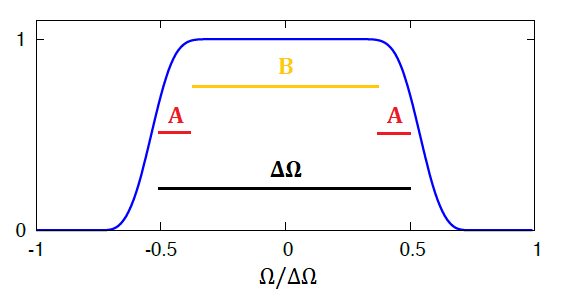
\includegraphics[width=0.6\textwidth,angle=0]{figures/phi_omega.png}
}
\caption{The window function for the WDM wavelets for the choice $d = 4$, $A =\Delta\Omega/4$ and $B = \Delta\Omega/2$. For this choice of window parameters the wavelets are better localized in frequency than they are in time. Here the overall normalization
is arbitrary.}
\label{fig:phi_omega}
\end{figure}
%
The free parameters to be chosen are $A$ and $d$, while all the others are defined consequently:
\begin{align}
\label{eq:window_bandwidth}
\Delta\Omega&=2\pi\Delta F\nonumber\\
B&=\Delta\Omega-2A.
\end{align}
We remark here that both $A$ and $B$ positive parameters. Next step, since the Meyer window function is built in the frequency domain, we can define the wavelet basis in the frequency domain
\begin{align}
\label{eq:gnm}
\tilde g_{mn}(\omega)=e^{-in\omega\Delta T}\left(C_{nm}\tilde\phi(\omega-m\Delta\Omega)+C^*_{nm}\tilde\phi(\omega+m\Delta\Omega)\right)
\end{align}
where $C_{nm}=1$ for $(n + m)$ even and $C_{nm}=i$ for $(n + m)$ odd.
(\textcolor{red}{Very unclear now how these coefficients})
From this point, there are two ways to compute the coefficients $w_{nm}$ of \eqref{wnm_def}, a slow one and a faster one.
\subsubsection{The slow method: $w_{nm}$ directly from the data stream}
\begin{itemize}
    \item We first of all anti-Fourier transform (\textcolor{red}{Please note that also this time, in both Cornish and Necula papers there's not a precise definition in terms of formulae for this passage}) the function $\tilde \phi(\omega)\to\phi(t)$.
    \item We cut the function $\phi(t)$ in the range $|t|<q\Delta T$ with $q$ another arbitrary quantity (Cornish set it to $q=16$ to produce the plots).
    \item For the discrete time samples of $s[k]$ we compute the weights (coefficients)
    \begin{align}
    \label{eq:direct}
w_{n m}=\sqrt{2} \Delta t \Re \left[C_{n m} \sum_{k=-K / 2}^{K / 2-1} e^{i \pi k m / N_f} x\left[n N_f+k\right] \phi[k]\right]\;,
\end{align}
where $K=2qN_f$
\end{itemize}
\subsubsection{The faster method: passing through $x_m[n]$ first}
\begin{itemize}
    \item We produce the discrete Fourier transform of the data stream $x[k]\to X[l]$
    \item We compute the "windowed-Fourier transforms"
    \begin{align}
    \label{eq:wdft}
        x_m[n]=\sum_{l=-N_t/2}^{N_t/2-1}e^{-2\pi iln/N_t}X[l+mN_t/2]\tilde\phi[l]
    \end{align}
    where we remind that the index $m$ runs over the frequency coordinates in the grid defined in \eqref{NtNf_def}, while $n$ runs over the time ones. \textcolor{red}{Note that according to the definition of the direct transform in \eqref{eq:direct} and the window Fourier transform in \eqref{eq:meyer_window_freq}, the wavelet transform $w_{nm}$ should have units of the square root of time. If we want the same to be true for \eqref{eq:wdft}, then the definition of the DFT \eqref{eq:dft-definition}should have a unit of time.}
    \item We compu$X$te the weights
    \begin{align}
    \label{eq:fast}
        w_{nm}=\sqrt{2}(-1)^{nm}\Re\left[C_{nm}x_m[n]\right]
    \end{align}
    \item \textbf{As an alternative}, accordingly to Cornish, the objects $x_m[n]$ "can be computed using a
    FFT of length $N_t$ for each $m$". \textcolor{red}{Again, the statement is cryptic and not supported by formulas. Necula did not mention even mention this method with the last formulas I have just written.} This alternative to the method is supposed to speed up the algorithm a lot (the total cost of the WDM transform would be less than twice the cost of the full FFT in this case). \textcolor{purple}{(Ollie:) I think this formula needs a $1/N_{t}$ in it. }
\end{itemize}

\subsection{Analytical Representation of Monochromatic Signals}
The purpose of this section is to derive analytical results for the time-domain, frequency domain and wavelet domain representation of a monochromatic signal.
\subsection{The time domain}
We choose to analyse the monochromatic signal
\begin{equation}\label{eq:simple_monochromatic_waveform}
y(t) = A\sin(2\pi f_{0} t)
\end{equation}
\textcolor{red}{[Giorgio] We can add a phase to be general} 
with constant amplitude and frequency $A, \ f_{0} \in \mathbb{R}$. In the language of signal processing, we sample the signal $y(t) \approx \{y[t_{j}]\}_{j=0}^{N_{t} - 1}$ with time bins $t_{j} = j\Delta t$ for sampling interval $\Delta t = t_{j} - t_{j-1}$. Here we use $N_{t}$ to dictate the number of time-bins such that $t_{N_{t}} = N_{t}\Delta t = T_{\text{obs}}$ for $T_{\text{obs}}$ the observation time. 
\textcolor{red}{[Giorgio] We should use $N$ and not $N_t$ for consistency with our notation I think} 

\subsubsection{The frequency domain}
To understand the wavelet domain, it helps to come back to the frequency domain and understand why the discrete time Fourier transform (DTFT) is just a special case of the WDM transformation. We will begin by discussing sampling of sinusoids with the goal of computing the DTFT of the monochromatic signal given by equation \eqref{eq:simple_monochromatic_waveform}. 

We define the discrete time Fourier transform\footnote{I will refer to the \textit{continuous} time Fourier transform as the discrete time Fourier transform but with an extra multiplicative factor $\Delta t$. From now on, however, I will work with the DTFT.} by 
\begin{align}\label{eq:dtft}
    \text{FFT}[y[n]] = \tilde{y}[f_{p}] &= \sum_{k = -N_{t}/2}^{N_{t}/2 - 1} y[k]\exp(-2\pi i f_{p}t_{k}) \\
    &= \sum_{k = -N_{t}/2}^{N_{t}/2 - 1} y[k]\exp(-2\pi i p k / N_{t})
\end{align}
Here $f_{p}$ is a discrete Fourier frequency with $f_{p} = p/T_{\text{obs}} = p/N_{t}\Delta t$. The number of discrete frequencies are given by the set $\{-N_{t}/2, -N_{t}/2 + 1, \ldots, -1, 0, 1, \ldots N_{t}/2\}$ such that there are precisely $N_{t}$ observable frequencies and the zeroth frequency bin has been shifted into the middle of the sum in \eqref{eq:dtft}. Note here that if one is to compute both positive and negative frequency transformations using \eqref{eq:dtft}, it is essential to use \texttt{np.fft.fftshift} prior to any Fourier transforms in \texttt{python}. Easy mistake to make! 

Before computing the DTFT of the monochromatic signal above \eqref{eq:simple_monochromatic_waveform}, it is useful to note the following identity: 
\begin{equation}\label{eq:dirichilet_identity_weird_sum}
\sum_{k = -N_{t}/2}^{N_{t}/2 - 1} \exp(i k x) = \frac{\sin(N_{t}x/2)}{\sin(x/2)}\,.
\end{equation}
This can be proved by induction or direct calculation. Notice that when $x \rightarrow 0$, the result of the above sum is $N_{t}$. This property will be used in the following calculations. 

To calculate the DTFT \eqref{eq:dtft} of the monochromatic signal \eqref{eq:simple_monochromatic_waveform}, we see that

\begin{align}
\tilde{y}[f_{p}] & =\sum_{k = -N_{t}/2}^{N_{t}/2 - 1} y[k]\exp(-2\pi i p k / N_{t}) \\
&= \frac{A}{2i}\sum_{k = -N_{t}/2}^{N_{t}/2 - 1} \left( e^{i\left[\frac{2\pi}{N_{t}}(m_{0} - p)\right]k} - e^{-i\left[\frac{2\pi}{N_{t}}(m_{0} - p)\right]k}\right)\,.
\end{align}
Here we define the integer $m_{0}$ such that the frequency $f_{0}$ in \eqref{eq:simple_monochromatic_waveform} satisfies $f_{0} = m_{0}/(N_{t}\Delta t)$. Now, the final equation above is in the same form as \eqref{eq:dirichilet_identity_weird_sum}, giving the final result for the DTFT
\begin{equation}\label{eq:tilde_y_analytical_form}
\tilde{y}[p] = \frac{A}{2i}\left(\frac{\sin[\pi(m_{0} - p)]}{\sin\left(\frac{\pi}{N_{t}}(m_{0} - p)\right)} - \frac{\sin[\pi(m_{0} + p)]}{\sin\left(\frac{\pi}{N_{t}}(m_{0} + p)\right)}\right).
\end{equation}
In the limit that $p \rightarrow \pm m_{0}$, we see that $\tilde{y}[p \rightarrow \pm m_{0}] = AN_{t}/(2i)$ as expected. Equation \eqref{eq:tilde_y_analytical_form} has been checked against python's internal \texttt{np.fft.fft} function and they agree to within machine precision. Even in the case of leakage.

We can write equation \eqref{eq:tilde_y_analytical_form} in the continuous limit. 
% Here is Quentin's derivation:
% \begin{eqnarray*}
%     \operatorname{F}_T[y](f) &=& \int_{-\frac{T}{2}}^{+\frac{T}{2}} A \sin(2\pi f_0 t) e^{-2 \pi f t} dt \\
%     & = & \frac{A}{2 i} \int_{-\frac{T}{2}}^{+\frac{T}{2}} \left[e^{2 i \pi (f_0 - f) t} - e^{-2 i \pi (f_0 + f) t} \right] dt \\
%     & = & \frac{A}{2 i} \left[\frac{e^{2 i \pi (f_0 - f) t}}{2 \pi i (f_0 - f)} + \frac{e^{-2 i \pi (f_0 + f) t}}{2 \pi i (f_0 + f)} \right]_{-\frac{T}{2}}^{\frac{T}{2}} \\
%     & = & \frac{A}{2 i} \left[\frac{e^{i \pi (f_0 - f) T} - e^{-i \pi (f_0 - f) T}}{2 \pi i (f_0 - f)} + \frac{e^{-i \pi (f_0 + f) T} - e^{i \pi (f_0 + f) T}}{2 \pi i (f_0 + f)} \right] \\
%     & = & \frac{A T}{2 i} \left[\operatorname{sinc}(\pi (f_0 -f) T ) - \operatorname{sinc}(\pi (f_0 + f) T ) \right]
% \end{eqnarray*}


% Notice that equation \eqref{eq:tilde_y_analytical_form} can be written as 

\begin{equation}
\tilde{y}(f_{p}) = \frac{A}{2i}\left(\frac{\sin[T_{\text{obs}}\pi(f_{0} - f_{p})]}{\sin\left(\Delta t \pi (f_{0} - f_{p})\right)} - \frac{\sin[T_{\text{obs}} \pi(f_{0} + f_{p})]}{\sin\left(\Delta t \pi(m_{0} + p)\right)}\right).
\end{equation}
Now, the DTFT is related to the CTFT by a multiplicative factor of $\Delta t$. Introducing this factor such that $\hat{y}(f_{p}) \approx \Delta t \cdot \tilde{y}(f)$ and expanding the denominator for small $\Delta t$, we would observe that 
\begin{equation}\label{eq:CTFT_expression}
\hat{y}(f_{p}) = \frac{A T_{\text{obs}}}{2i}\left(\frac{\sin[T_{\text{obs}}\pi(f_{0} - f_{p})]}{T\pi (f_{0} - f_{p})} - \frac{\sin[T_{\text{obs}} \pi(f_{0} + f_{p})]}{T \pi(m_{0} + p)}\right)\, ,
\end{equation}
which then simplifies to the continuous expression 
\begin{equation}
\label{eq:CTFT_expression_monochromatic_signal}
\hat{y}(f) = \frac{A T_\text{obs}}{2i}\left\{\text{sinc}[\pi(f_{0} - f)T_{\text{obs}}] - \text{sinc}[\pi(f_{0} + f)T_{\text{obs}} ]\right\}\,,
\end{equation}
with the $\text{sinc}$ function defined by 
\begin{equation}
    \text{sinc}(\pi x) = \frac{\sin (\pi x)}{\pi x }\, ,
\end{equation}
with the useful identity that $\lim_{x \rightarrow 0} \text{sinc}(\pi x) = 1$. Now, using the result of \eqref{eq:CTFT_expression_monochromatic_signal}, we will try to convert the monochromatic expression \eqref{eq:simple_monochromatic_waveform} into the wavelet domain. 

\textcolor{red}{
[Giorgio] Good news is that this equation can be obtained equivalently by directly performing the integration in the continuous domain
%
\begin{align}
\hat y(f)=\int_{-T_{\rm obs}/2}^{T_{\rm obs}/2} dt A\sin(2\pi f_0 t) e^{-2\pi i f t}=\frac{i A (f \cos (\pi  f T_\text{obs}) \sin (\pi f_0 T_\text{obs})-f_0 \sin (\pi  f T_\text{obs}) \cos (\pi  f_0 T_\text{obs}))}{\pi  \left(f^2-f_0^2\right)}
\end{align}
%
and then one can check (just a bit of algebra or the help of Mathematica) that it is the same expression of \ref{eq:CTFT_expression_monochromatic_signal}
}



% What's wrong with the equation below? Or what's wrong with what I have?
% In the continuous limit (but finite time series with observation time $T$), Eq.~\eqref{eq:tilde_y_analytical_form} becomes
% \begin{equation}\label{eq:tilde_y_analytical_form_continuous}
% \tilde{y}[f] \approx \frac{A T }{2i}\left( e^{i\pi(f_0-f)} \operatorname{sinc}(\pi(f_0-f)T) - e^{-i\pi(f_0+f)} \operatorname{sinc}(\pi(f_0+f_p)T) \right).
% \end{equation}


\subsubsection{The wavelet domain}\label{subsubsec:monchromatic_wavelet_calculations}
Now, we can try to use the results above to compute an analytical result for each of the $w_{nm}$ wavelet coefficients. Recall from From Cornish's paper, we see that if the signal in the Fourier domain is known, it is cheaper and (apparently) easier to compute the $w_{nm}$ values from 
\begin{align}
w_{nm} &= \sqrt{2}(-1)^{nm}\mathcal{R} (C_{nm}x_{m}[n])\label{eq:w_nm}\\
x_{m}[n] & = \frac{1}{N_{t}}\sum_{l = -N_{t}/2}^{N_{t}/2 - 1} \exp(-2\pi i l n / N_{t}) \tilde{X}[l + mN_{t}/2]\Psi[l]\label{eq:xmn_ifft}
\end{align}
for $\Psi$ a normalised frequency domain Meyer-wavelet I will introduce later. Equation \eqref{eq:xmn_ifft} can be thought of as a windowed inverse discrete Fourier transform. Note here that we have introduced a factor $1/N_{t}$ into \eqref{eq:xmn_ifft} that is not present in Cornish's original formula. I firmly believe that this is a typo in Cornish's paper. 

Now, we can proceed with computing an expression for a monochromatic signal \eqref{eq:simple_monochromatic_waveform} in the wavelet domain using equations \eqref{eq:w_nm} and \eqref{eq:xmn_ifft}. We have derived an expression for discrete Fourier transform of the data $\tilde{X}$ above in \eqref{eq:tilde_y_analytical_form}. Consider the product
\begin{align}
e^{-2\pi i ln/N_{t}}\tilde{X}[l + mN_{t}/2] &= \frac{A}{2i}e^{-2\pi i ln/N_{t}}\left(\frac{\sin[\pi(m_{0} - l - mN_{t}/2)]}{\sin\left(\frac{\pi}{N_{t}}(m_{0} - l - mN_{t}/2 )\right)} - [p \mapsto -p]\right) \nonumber\\
& = \frac{A}{2i}\left(\frac{e^{2\pi i \left(\frac{m_{0} - l}{2} - \frac{mN_{t}}{4}\right)} - e^{-2\pi i \left(\frac{m_{0} - l}{2} - \frac{mN_{t}}{4}\right)}}{e^{\frac{2\pi i}{N}\left(\frac{m_{0} - l}{2} - \frac{mN_{t}}{4} + \frac{lnN}{N_{t}}\right)} - e^{-\frac{2\pi i}{N}\left(\frac{m_{0} - l}{2} - \frac{mN_{t}}{4} + \frac{lnN}{N_{t}}\right)}} - [p \mapsto -p]\right)\nonumber
\end{align}
where $p \mapsto -p$ gives the other term in the expressions above such that $l + mN_{t}/2 \mapsto -l - mN_{t}/2$. Now, understand that the only way for the expression above to be non-zero is if \textcolor{red}{[Giorgio] Why?} 
\begin{align}
\frac{m_{0} - l}{2} - \frac{mN_{t}}{4} &= 0 \\
\frac{m_{0} - l}{2} - \frac{mN_{t}}{4} + \frac{lnN}{N_{t}} &= 0\,,
\end{align}
which admits the unique (?) solution $l = 0$ and $m = 2m_{0}/N_{t}$. For the $p\mapsto -p$, we have the same solution but for $l = 0$ and $m = -2m_{0}/N_{t}$. Understand here that this specific $m$ index corresponds to the frequency $f_{0}$ in the wavelet domain. Fixing $m = 2m_{0}/N_{t}$ and substituting into the expression we find 
\begin{align}
x_{m}[n] = \frac{1}{N_{t}} \sum_{l = -N_{t}/2}^{N_{t}/2 - 1} \frac{A}{2i}\left(\frac{e^{-i\pi l} - e^{i\pi l}}{e^{\frac{2\pi i l}{N}\left(\frac{1}{2} + \frac{nN}{N_{t}}\right)} - e^{-\frac{2\pi i l}{N}\left(\frac{1}{2} + \frac{nN}{N_{t}}\right)}}\right) \Phi[l] \,,
\end{align}
The only non-zero value in this expression is the value at precisely $l = 0$. Taking the limit $l \rightarrow 0$ and Taylor expanding the exponentials yields
\begin{align}\label{eq:x_mn_monochromatic_Psi}
x_{m}[n] = \frac{A N_{f}}{2i} \Psi[l = 0]. \,,
\end{align}
Now, at this point, I am going to define $\Psi(\omega)$ in precisely the same way as in our code. Defining $\Delta F = 1/(2N_{f})$ and $\Delta \Omega = 2\pi \Delta F$, we will build a \emph{normalised} meyer-wavelet in the following way
\begin{equation}
\Psi[l] = \sqrt{\frac{N}{2\left[2\sum_{l = 1}^{N_{t}/2 - 1}\tilde{\phi}[l]^2 + \phi[l= 0]^2\right]}} \cdot \frac{2}{N_{f}} \tilde{\phi}[l].
\end{equation}
This is what is presented in the code. Interestingly, the above equation can be simplified dramatically. I believe it's possible to show that
\begin{equation}
2\sum_{l = 1}^{N_{t}/2 - 1}\tilde{\phi}[l]^2 + \phi[l= 0]^2 = \frac{N_{t}}{2\Delta\Omega} = \frac{N}{2\pi}.
\end{equation}
Hence, we recover a massive simplification\footnote{I have no idea why this is not just set in the code...}
\begin{equation}\label{eq:normalised_meyer_wavelet}
\Psi[l] = \left(\frac{2}{N_{f}}\sqrt{\pi}\right)\tilde{\phi}[l].
\end{equation}
The part in brackets above is precisely the normalisation constant that is used in our code. Here $\tilde{\phi}[l]$ is defined in the same way as \eqref{eq:meyer_window_freq}. We note here the maximum value of $\Psi[l]$ is given when $l = 0$, i.e.,
\begin{align}\label{eq:psi_l=0_normed}
   \Psi[l = 0] = \left(\frac{2}{N_{f}}\sqrt{\pi}\right) \cdot \frac{1}{\sqrt{\Delta\Omega}} = \left(\frac{2}{N_{f}}\sqrt{\pi}\right) \sqrt{\frac{N_{f}}{\pi}} = \frac{2}{\sqrt{N_{f}}}.
\end{align}

To complete our calculation, we can substitute \eqref{eq:normalised_meyer_wavelet} with $l = 0$ into \eqref{eq:x_mn_monochromatic_Psi} giving
\begin{equation}
x_{m}[n] = \frac{A\sqrt{N_{f}}}{i}, \quad (l = 0) \ \wedge \ (m = 2m_{0}/N_{t}) \wedge \forall n .
\end{equation}
Substituting this into Equation \eqref{eq:w_nm} giving the wavelet coefficients, $\omega_{nm}$, we obtain
\begin{equation}
\omega_{nm} =(-1)^{nm}\text{Re}\left[\frac{C_{nm}A\sqrt{2N_{f}}}{i}\right].
\end{equation}
The only non-zero values in this equation are for $C_{nm} = i$, which only happens when $(n + m)$ is an odd integer. If $(n+m)$ is odd, then one of $n$ and $m$ must be odd or even but neither both. This implies there is no oscillation in the wavelet coefficients, i.e., $(-1)^{nm} = 1$. The wavelet coefficients are thus given by 
\begin{equation}\label{eq:w_mn_monochrom_signal_finished}
\omega_{nm} = 
\begin{cases}
     0 & \text{if } n \in 2\mathbb{Z}_{\geq 0} \ \wedge \forall m\\
    A\sqrt{2 N_{f}} & n \in 2\mathbb{Z}_{\geq 0} + 1 \ \wedge  m = 2m_{0}/N_{t} \in 2\mathbb{Z}_{\geq 0}
\end{cases}
\end{equation}
As an example using the code, we can generate the spectrogram of a monochromatic signal with $A = 2$, $f_{0} = 20Hz$ sampled with cadence $\Delta t = 0.0125$. The observation time is $T_{\text{obs}} = 1000$ seconds. The signal is zero-padded to the next integer power of two giving $N = 2^{16}$ samples in the time-domain. In this example, we set $N_{f} = 512$ frequency slices giving $N_{t} = 128$ time slices in the wavelet domain. We construct the wavelet-domain representation of the monochromatic signal using both \eqref{eq:w_nm} and \eqref{eq:x_mn_monochromatic_Psi}. The resulting matrix $\omega_{nm}$ is sparse, resulting in a single row of non-zero values. This single row is precisely the index $m = 256$ that indicates $f_{0} = 20$. Only the $n = \{1,3,\ldots, N_{t}-1\}$ time indices give non-zero values. Finally, for each of these values, the value of the wavelet coefficients are $\omega_{nm} \approx 64 = 2\cdot \sqrt{2\cdot 512} = 2\cdot 32 = 64$. This value agrees with the formula presented in \eqref{eq:w_mn_monochrom_signal_finished}. % This latter equation can be written in the continuous domain. Observe that 
% \begin{equation}
% x_{m}(t) \approx T_{\text{obs}} \int_{-\infty}^{\infty} e^{-2\pi i f t}X(f + m f_{\text{nyq}}) \Phi(f) \, \text{d}f
% \end{equation}
% Suppose we have a signal of the form 
% \begin{equation}
% h = A \sin(2\pi f_{0} t)
% \end{equation}
\begin{figure}
\centering
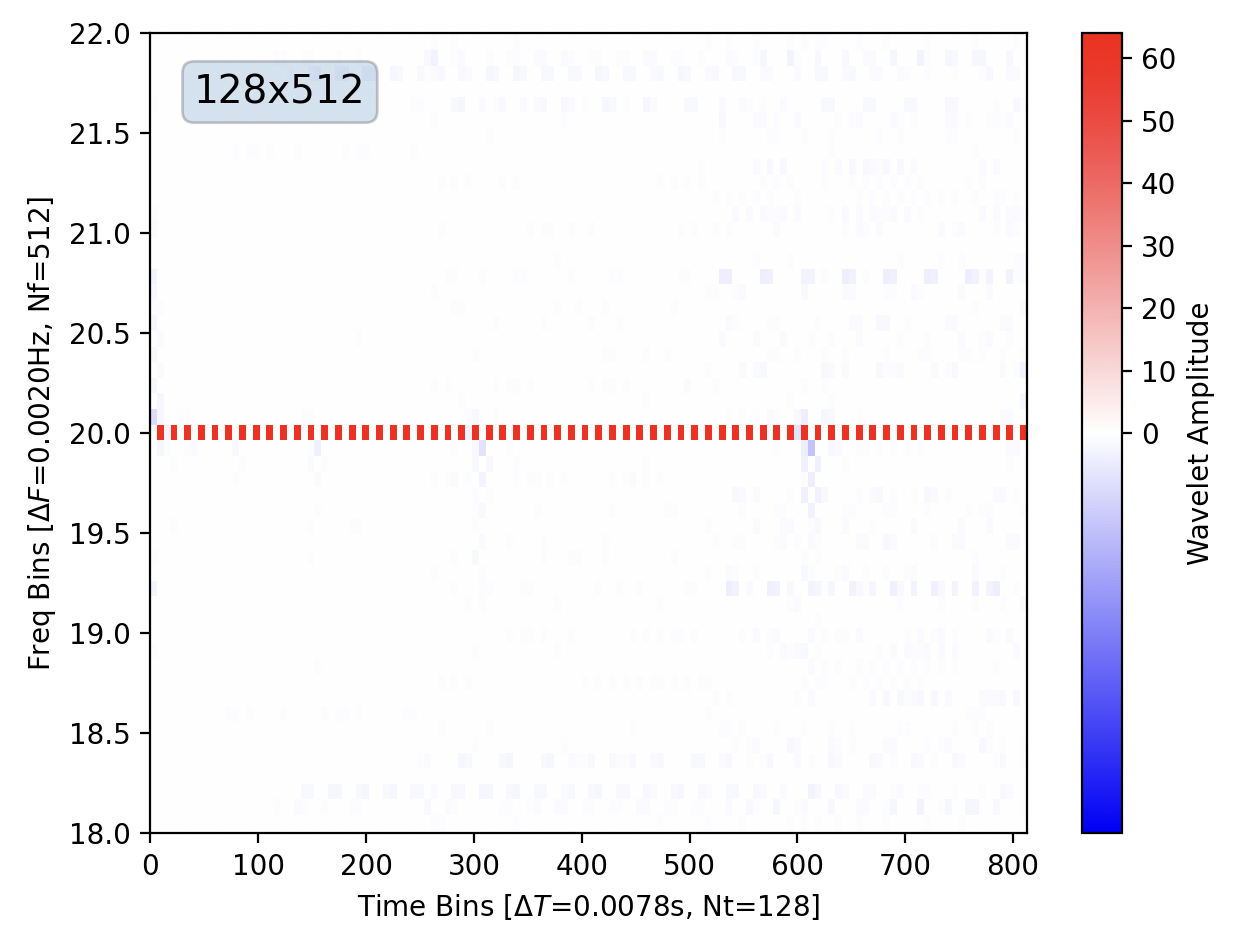
\includegraphics[width = 0.75\textwidth]{figures/Monochromatic_Signal/Spectrogram.png}
\caption{Spectrogram of the monochromatic signal given in equation \eqref{eq:simple_monochromatic_waveform} using equations \eqref{eq:w_nm} and \eqref{eq:x_mn_monochromatic_Psi}. The maximum amplitude is indeed given by \eqref{eq:w_mn_monochrom_signal_finished} and gives $\omega_{mn} = A\sqrt{2N_{f}} = 64$ for $m$ even and $n$ odd}
\label{fig:hello}
\end{figure}
% I claim that the wavelet coefficients are equal to 
% \begin{equation}
% \omega_{nm} = 
% \begin{cases}
%      0 & \text{if } n \in 2\mathbb{Z}_{\geq 0} \ \wedge \forall m\\
%     A\sqrt{2 N_{f}} & n \in 2\mathbb{Z}_{\geq 0} + 1 \ \wedge  m = k\Delta F
% \end{cases}
% \end{equation}
% for $k\Delta F = f_{0}$. This agrees with the formula for the SNR in the wavelet domain 
% \begin{equation}
% \rho^2 _{\text{wavelet}} = \sum_{nm}\frac{\omega_{nm } \cdot \omega_{nm}}{S_{nm}}
% \end{equation}
% for the denominator given by the evolutionary PSD and the numerator the pointwise multiplication (and sum). Substituting the above wavelet coefficients into the SNR formula gives

% \begin{align}
% \rho^{2}_\text{wavelet} = \frac{A^{2} 2 N_{f} [N_{t}/2]}{S_{nm}} \approx \frac{A^{2} N_{f} N_{t}}{S(f_{0})/\Delta t} 
%  = \frac{A^{2} N\Delta t}{S(f_{0})} 
%  = \frac{A^2 T}{S(f_{0})}\,,
% \end{align}
% which is the same analytical SNR formula reached when using parseval's theorem. In the first equality, there are only $N_{t}/2$ non-zero values hence the factor of $N_{t}/2$. We have also used the approximation that $S(f_{m},t_{n}) = S(f_{m})/\Delta t$. 




\section{Statistics of wavelet coefficients}

% \subsection{With stationary noise}

% In this section, we assume that the time series $x[k]$ is a realization of the stationary, zero-mean Gaussian noise of one-sided power spectral density (PSD) $S(f)$. We wish to derive the approximate covariance of the wavelet coefficients $w_{nm}$. We start from Eqs.~\eqref{eq:wdft} and \eqref{eq:fast} and compute the covariance of two wavelet coefficients. Let us define the complex quantity $\underbar{w}_{nm}$ the same way as $w_{nm}$ in Eq.~\eqref{eq:fast} but without the real part operator. We have
% \begin{align}
% \label{eq:covariance_1}
%     \operatorname{E}\left[\underbar{w}_{nm} \underbar{w}_{n'm'}^{\ast}\right] = 2 C_{n m}  C_{n' m'}^{\ast} \sum_{l=-N_t / 2}^{N_t / 2-1} \sum_{l'=-N_t / 2}^{N_t / 2-1}   e^{-2 i \pi (ln  - l' n' )/ N_t} \operatorname{E}\left[ X\left[l + m N_t / 2 \right] X\left[l' + m' N_t / 2 \right]^{\ast}  \right] \tilde{\phi}[l] \tilde{\phi}[l']^{\ast}
% \end{align}
% Using the circulant approximation of the stationary time series covariance, we have
% \begin{align}
%     \operatorname{E}\left[X[k]X[k']^{\ast}\right] \approx \delta_{k k'} \frac{N}{2 \Delta t}S(f_k),
% \end{align}
% where $f_k = k / T$. The prefactor comes from the fact that we assumed no special normalization of the discrete Fourier transform $X$ like in Eq.~\eqref{eq:dft-definition}. \textcolor{red}{However, if we want the wavelet coefficients to have units of the square root of time, we need to add a $\Delta t$ factor in this definition.} This yields
% \begin{align*}
%     \operatorname{E}\left[X[k]X[k']^{\ast}\right] \approx \delta_{k k'} \frac{N\Delta t}{2}S(f_k) = \delta_{k k'} \frac{T}{2}S(f_k),
% \end{align*}
% Therefore, the expectation term in Eq.~\eqref{eq:covariance_1} is non-zero only when 
% \begin{align}
% \label{eq:lconditions}
%     l + m N_t / 2 & = l' + m' N_t / 2 \text{ or} \nonumber \\
%     l + m N_t / 2 & = N_t - l' - m' N_t / 2.
% \end{align}
% The index $l' = l^{\prime}_0 = l + (m-m') N_t / 2$ verifies the first equality in Eqs.\eqref{eq:lconditions}. There are only two non-zero terms in the sum over $l'$ corresponding to $l^{\prime}_0$ and $N_t - l^{\prime}_0$. Eq.~\eqref{eq:covariance_1}  becomes
% \begin{align}
% \label{eq:covariance_2}
%     \operatorname{E}\left[\underbar{w}_{nm} \underbar{w}_{n'm'}^{\ast}\right] & \approx 2 C_{n m}  C_{n' m'}^{\ast} \sum_{l=-N_t / 2}^{N_t / 2-1}   e^{-2 i \pi (ln  - (l + (m-m')N_t/2 )n' )/ N_t} \frac{N}{2 \Delta t}S\left( f_{l + m N_t / 2} \right)  \nonumber \\
%     & \times \tilde{\phi}[l] \left(\tilde{\phi}[l + (m-m') N_t / 2]^{\ast} + \tilde{\phi}[-l + (2 - m + m') N_t / 2]^{\ast} \right)
% \end{align}

% From Eq.~\eqref{eq:meyer_window_freq} we see that the Meyer window function $\tilde\phi(\omega)$ is non-zero for angular frequencies such that $|\omega| < \Delta \Omega $. Using Eq.~\eqref{eq:window_bandwidth}, the frequency indices $l$ corresponding to this condition are
% \begin{align}
% \label{eq:bandwidth-condition}
%     \left| \frac{2 \pi l}{T} \right| \leq 2 \pi \Delta F.
% \end{align}
% Eq.~\eqref{eq:covariance_2} exhibits the product $\tilde{\phi}[l] \tilde{\phi}[l + (m-m') N_t / 2]^{\ast}$. Let us assume that the window is zero outside the bandwith $\Delta \Omega$ (which is approximately true) and equal to $1/\sqrt{\Omega}$ inside. Then the product takes non-zero values only if $l$ and $l + (m-m') N_t / 2$ simultaneously satisfy the condition \eqref{eq:bandwidth-condition}, which is only possible if $m=m'$. The same is true for the second product. As a result, two wavelet frequency bins are approximately uncorrelated.

% Furthermore, from the relations in Eq.~\eqref{NtNf_def} and Eq.\eqref{DTDF} we can express $\Delta F = 1 / (2 \Delta t N_f) = N_t / (2 \Delta t N)$ to check that the condition \eqref{eq:bandwidth-condition} is strictly equivalent to $|l| \leq N_t / 2$. Therefore, Eq.~\eqref{eq:covariance_2} becomes
% \begin{align}
% \label{eq:covariance_3}
%     \operatorname{E}\left[\underbar{w}_{nm} \underbar{w}_{n'm'}^{\ast}\right] & \approx \frac{2 N}{\Delta t} \delta_{m m'} C_{n m}  C_{n' m}^{\ast} \sum_{l=-N_t / 2}^{N_t / 2-1}   e^{-2 i \pi l (n-n') / N_t} S\left(f_{l + m N_t / 2}\right)  | \tilde{\phi}[l] |^{2} 
% \end{align}
% The above expression is a circuclar convolution of the PSD with some kernel 
% \begin{align}
%     K_{n, n', m}[l] &  \equiv \frac{2 N}{\Delta t} C_{n m}  C_{n' m}^{\ast} | \tilde{\phi}[l] |^{2}  e^{-2 i \pi l (n-n') / N_t}.
% \end{align}
% If we Taylor-expand the PSD around the central frequency $f_{m M_t/2}$, we get
% \begin{align}
% \label{eq:covariance_4}
%     \operatorname{E}\left[\underbar{w}_{nm} \underbar{w}_{n'm'}^{\ast}\right] & \approx \delta_{mm'} \sum_{l=-N_t / 2}^{N_t / 2-1}    K_{n, n', m}[l] \left( S\left(f_{m N_t / 2}\right) + \frac{l}{T} S'\left(f_{m N_t / 2}\right)  + \frac{l^2}{2T^2} S^{\prime\prime}\left(f_{m N_t / 2}\right) \right),
% \end{align}
% where $S^{q}$ is the $q^{\mathrm{th}}$ derivative of the PSD with respect to frequency. If we assume that over the frequency bandwidth $\Delta F$, the window function is always equal to $1/\sqrt{2 \pi \Delta F}$ in Eq.~\eqref{eq:meyer_window_freq}, then at zeroth order we have
% \begin{align}
% \label{eq:covariance_order_0}
%     \operatorname{E}\left[\underbar{w}_{nm} \underbar{w}_{n'm'}^{\ast}\right] & \approx \frac{2 N}{\Delta t} \delta_{m m'} C_{n m}  C_{n' m}^{\ast} S\left(f_{m N_t / 2}\right) \frac{1}{2 \pi \Delta F}  \sum_{l=-N_t / 2}^{N_t / 2-1}   e^{-2 i \pi l (n-n') / N_t} 
% \end{align}
% The geometric sum over $l$ is then equal to $N_t$ if $n = n'$, and zero otherwise. Consequently, the wavelet covariance matrix can be considered diagonal with terms given by 
% \begin{align}
% \label{eq:covariance_order_0_diag}
%     \operatorname{E}\left[\underbar{w}_{nm} \underbar{w}_{n'm'}^{\ast}\right] & \approx \delta_{m m'} \delta_{n n'}  \frac{N}{\Delta t}\frac{N_t}{\pi \Delta F}  S\left(f_{m N_t / 2}\right) ,
% \end{align}
% where we have used the fact that $|C_{n m}|^{2} = 1$. Using the relation $\Delta F = N_t / (2 T)$ from Eq.~\eqref{eq:window_bandwidth}, we get
% \begin{align}
% \label{eq:covariance_order_0_diag2}
%     \operatorname{E}\left[\underbar{w}_{nm} \underbar{w}_{n'm'}^{\ast}\right] & \approx \delta_{m m'} \delta_{n n'} \frac{N}{\Delta t}\frac{2T}{\pi}   S\left(f_{m N_t / 2}\right) \nonumber \\
%     & = \delta_{m m'} \delta_{n n'}  \frac{2 N^2}{\pi}  S\left(f_{m N_t / 2}\right) \nonumber
% \end{align}
% We assumed that the underlying process was zero-mean Gaussian so that $\operatorname{E}[\underbar{w}_{nm}] = 0$ and $\underbar{w}_{nm}$ is a circularly symmetric random variable. Therefore, we have 
% \begin{align}
%    \operatorname{E}\left[w_{nm} w_{n'm'}\right] =  \operatorname{E}\left[\Re \underbar{w}_{nm} \Re \underbar{w}_{n'm'}^{\ast}\right] & = \frac{1}{2} \Re \left\{ \operatorname{E}\left[\underbar{w}_{nm} \underbar{w}_{n'm'}^{\ast}\right] \right\}
% \end{align}
% Therefore, at zeroth order we get 
% \begin{align}
% \label{eq:covariance_wnm}
%    \operatorname{E}\left[w_{nm} w_{n'm'}\right] & =  \delta_{m m'} \delta_{n n'}  \frac{N^2}{\pi}  S\left(f_{m N_t / 2}\right)
% \end{align}
% Note that the first-order sum in Eq.~\eqref{eq:covariance_4} is actually zero, meaning that the error when making the approximation in Eq.~\eqref{eq:covariance_wnm} will depend on the second derivative of the likelihood. Also, the prefactor we get in front of the PSD is not the same as in Eq. (19) of Cornish et al 2020. But this depends on the normalization of the discrete Fourier transform. However, regardless of the DFT normalization, Eq.~(19) does not seem compatible with the way the window function $\phi$ has been defined. \ob{Is this section necessary? Particularly given \ref{sec:locally_statioanry} below?}
% \begin{align}
% \label{eq:direct}
% w_{n m}=\sqrt{2} \Delta t \Re \left[C_{n m} \sum_{k=-K / 2}^{K / 2-1} e^{i \pi k m / N_f} x\left[n N_f+k\right] \phi[k]\right]\;,
% \end{align}
\subsection{With stationary noise (with new window)}

In this section, we assume that the time series $x[k]$ is a realization of the stationary, zero-mean Gaussian noise of one-sided power spectral density (PSD) $S(f)$. We wish to derive the approximate covariance of the wavelet coefficients $w_{nm}$. We start from Eqs.~\eqref{eq:wdft} and \eqref{eq:fast} and compute the covariance of two wavelet coefficients. Let us define the complex quantity $\underbar{w}_{nm}$ the same way as $w_{nm}$ in Eq.~\eqref{eq:fast} but without the real part operator. We have
\begin{align}
\label{eq:covariance_1}
    \operatorname{E}\left[\underbar{w}_{nm} \underbar{w}_{n'm'}^{\ast}\right] = \frac{2}{N_{t}^2} C_{n m}  C_{n' m'}^{\ast} \sum_{l=-N_t / 2}^{N_t / 2-1} \sum_{l'=-N_t / 2}^{N_t / 2-1}   e^{-2 i \pi (ln  - l' n' )/ N_t} \operatorname{E}\left[ X\left[l + m N_t / 2 \right] X\left[l' + m' N_t / 2 \right]^{\ast}  \right] \tilde{\Psi}[l] \tilde{\Psi}[l']^{\ast}
\end{align}
Using the circulant approximation of the stationary time series covariance, we have
\begin{align}
    \operatorname{E}\left[X[k]X[k']^{\ast}\right] \approx \delta_{k k'} \frac{N}{2 \Delta t}S(f_k),
\end{align}
where $f_k = k / T$. The prefactor comes from the fact that we assumed no special normalization of the discrete Fourier transform $X$ like in Eq.~\eqref{eq:dft-definition}. If we were to use the dimensionful discrete Fourier transform $\tilde{X}\mapsto \Delta t \tilde{X}$, one would obtain
\begin{align*}
    \operatorname{E}\left[X[k]X[k']^{\ast}\right] \approx \delta_{k k'} \frac{N\Delta t}{2}S(f_k) = \delta_{k k'} \frac{T}{2}S(f_k),
\end{align*}
Therefore, the expectation term in Eq.~\eqref{eq:covariance_1} is non-zero only when 
\begin{align}
\label{eq:lconditions}
    l + m N_t / 2 & = l' + m' N_t / 2 \text{ or} \nonumber \\
    l + m N_t / 2 & = N_t - l' - m' N_t / 2.
\end{align}
The index $l' = l^{\prime}_0 = l + (m-m') N_t / 2$ verifies the first equality in Eqs.\eqref{eq:lconditions}. There are only two non-zero terms in the sum over $l'$ corresponding to $l^{\prime}_0$ and $N_t - l^{\prime}_0$. Eq.~\eqref{eq:covariance_1}  becomes
\begin{align}
\label{eq:covariance_2}
    \operatorname{E}\left[\underbar{w}_{nm} \underbar{w}_{n'm'}^{\ast}\right] & \approx \frac{2}{N_{t}^2} C_{n m}  C_{n' m'}^{\ast} \sum_{l=-N_t / 2}^{N_t / 2-1}   e^{-2 i \pi (ln  - (l + (m-m')N_t/2 )n' )/ N_t} \frac{N}{2 \Delta t}S\left( f_{l + m N_t / 2} \right)  \nonumber \\
    & \times \Psi[l] \left(\Psi[l + (m-m') N_t / 2]^{\ast} + \Psi[-l + (2 - m + m') N_t / 2]^{\ast} \right)
\end{align}

From Eq.~\eqref{eq:meyer_window_freq} we see that the Meyer window function $\Psi(\omega)$ is non-zero for angular frequencies such that $|\omega| < \Delta \Omega $. Using Eq.~\eqref{eq:window_bandwidth}, the frequency indices $l$ corresponding to this condition are
\begin{align}
\label{eq:bandwidth-condition}
    \left| 2 \pi l \right| \leq 2 \pi \Delta F.
\end{align}
Eq.~\eqref{eq:covariance_2} exhibits the product $\Psi[l] \Psi[l + (m-m') N_t / 2]^{\ast}$. Let us assume that the window is zero outside the bandwith $\Delta \Omega$ (which is approximately true) and equal to $1/\sqrt{\Delta\Omega}$ inside. Then the product takes non-zero values only if $l$ and $l + (m-m') N_t / 2$ simultaneously satisfy the condition \eqref{eq:bandwidth-condition}, which is only possible if $m=m'$. The same is true for the second product. As a result, two wavelet frequency bins are approximately uncorrelated.

Furthermore, from the (code specific!!) relations we can express $\Delta F = 1 / (2 N_f)$ to check that the condition \eqref{eq:bandwidth-condition} is strictly equivalent to $|l| \leq N_t / 2$. Therefore, Eq.~\eqref{eq:covariance_2} becomes
\begin{align}
\label{eq:covariance_3}
    \operatorname{E}\left[\underbar{w}_{nm} \underbar{w}_{n'm'}^{\ast}\right] & \approx \frac{N}{N_{t}^2\Delta t} \delta_{m m'} C_{n m}  C_{n' m}^{\ast} \sum_{l=-N_t / 2}^{N_t / 2-1}   e^{-2 i \pi l (n-n') / N_t} S\left(f_{l + m N_t / 2}\right)  | \Psi[l] |^{2} 
\end{align}
The above expression is a circuclar convolution of the PSD with some kernel 
\begin{align}
    K_{n, n', m}[l] &  \equiv \frac{N}{N_{t}^2\Delta t} C_{n m}  C_{n' m}^{\ast} | \Psi[l] |^{2}  e^{-2 i \pi l (n-n') / N_t}.
\end{align}
If we Taylor-expand the PSD around the central frequency $f_{m M_t/2}$, we get
\begin{align}
\label{eq:covariance_4}
    \operatorname{E}\left[\underbar{w}_{nm} \underbar{w}_{n'm'}^{\ast}\right] & \approx \delta_{mm'} \sum_{l=-N_t / 2}^{N_t / 2-1}    K_{n, n', m}[l] \left( S\left(f_{m N_t / 2}\right) + \frac{l}{T} S'\left(f_{m N_t / 2}\right)  + \frac{l^2}{2T^2} S^{\prime\prime}\left(f_{m N_t / 2}\right) \right),
\end{align}
where $S^{q}$ is the $q^{\mathrm{th}}$ derivative of the PSD with respect to frequency. If we assume that over the frequency bandwidth $\Delta F$, the window function \eqref{eq:psi_l=0_normed} is always equal to $2/\sqrt{N_{f}}$ in Eq.~\eqref{eq:meyer_window_freq}, then at zeroth order we have
\begin{align}
\label{eq:covariance_order_0}
    \operatorname{E}\left[\underbar{w}_{nm} \underbar{w}_{n'm'}^{\ast}\right] & \approx \frac{N}{N_{t}^2\Delta t} \delta_{m m'} C_{n m}  C_{n' m}^{\ast} S\left(f_{m N_t / 2}\right)\frac{4}{N_{f}}  \sum_{l=-N_t / 2}^{N_t / 2-1}   e^{-2 i \pi l (n-n') / N_t} 
\end{align}
The geometric sum over $l$ is then equal to $N_t$ if $n = n'$, and zero otherwise. Consequently, the wavelet covariance matrix can be considered diagonal with terms given by 
\begin{align}
\label{eq:covariance_order_0_diag}
    \operatorname{E}\left[\underbar{w}_{nm} \underbar{w}_{n'm'}^{\ast}\right] & \approx \delta_{m m'} \delta_{n n'}  \frac{N}{N_{t}^2\Delta t}\frac{4N_t}{N_{f}} S\left(f_{m N_t / 2}\right) ,
\end{align}
where we have used the fact that $|C_{n m}|^{2} = 1$. Using the relation $N = N_{t}N_{f}$, we get
\begin{align}
\label{eq:covariance_order_0_diag2}
    \operatorname{E}\left[\underbar{w}_{nm} \underbar{w}_{n'm'}^{\ast}\right] & \approx \delta_{m m'} \delta_{n n'} \frac{4}{\Delta t} S(f_{mN_{t}/2})  
\end{align}
We assumed that the underlying process was zero-mean Gaussian so that $\operatorname{E}[\underbar{w}_{nm}] = 0$ and $\underbar{w}_{nm}$ is a circularly symmetric random variable. Therefore, we have 
\begin{align}
   \operatorname{E}\left[w_{nm} w_{n'm'}\right] =  \operatorname{E}\left[\Re \underbar{w}_{nm} \Re \underbar{w}_{n'm'}^{\ast}\right] & = \frac{1}{2} \Re \left\{ \operatorname{E}\left[\underbar{w}_{nm} \underbar{w}_{n'm'}^{\ast}\right] \right\}
\end{align}
Therefore, at zeroth order we get 
\begin{align}
\label{eq:covariance_wnm}
   \operatorname{E}\left[w_{nm} w_{n'm'}\right] & =  \delta_{m m'} \delta_{n n'}  \frac{2}{\Delta t}  S\left(f_{m N_t / 2}\right).
\end{align}
\textcolor{purple}{I'm still out by a factor of $2$ here... not sure why. Could it just be a one/two-sided PSD convention?} 


\subsection{With locally stationary noise}\label{sec:locally_statioanry}

In this section we will use concepts exposed in \cite{mallat_adaptive_1998}.

\subsubsection{Definition}
Let us consider a stochastic process $x$ with covariance 
\begin{eqnarray}
    R(t, s) = \operatorname{E}\left[x(t) x(s)\right].
\end{eqnarray}
We say that $x$ is a locally stationary process if in the neighbourhood of any point $\tau$ there exists an interval of size $l(\tau)$ and a length $d(\tau) < l(\tau)/2$ so that
\begin{align}
\label{eq:locally-stationary}
R(t, s)  \approx \left\{
\begin{array}{lr}
C(\tau, t-s) & \text { if }|t-s| \leq \frac{l(\tau)}{2}\\
0 & \text { if }|t-s| > d(\tau).
\end{array}\right.\;
\end{align}
where $C$ is a function and $\tau = (t-s) / 2$ is the mid-point between $t$ and $s$.
It is then useful to define a time-varying spectrum $S$ so that
\begin{align}
\label{eq:def-evolutionary-spectrum}
S(u, f) & = \int_{-\infty}^{+\infty} R\left(u+\frac{v}{2}, u-\frac{v}{2}\right) e^{-2 i \pi f  v} d v
\end{align}
We can also express it as the function $C$ defined so that $R(t, s) = C((t+s)/2, t-s)$:
\begin{align}
\label{eq:def-evolutionary-spectrum-2}
S(u, f) & = \int_{-\infty}^{+\infty} C(u, v) e^{-2 i \pi f  v} d v
\end{align}


With this definition, for any frequency $\xi$, the time-varying spectrum $S(u, f)$ of a locally stationary process can we approximated by a constant $S(\tau, \xi)$ in the time-frequency rectangle
\begin{eqnarray}
\label{eq:constant_spectrum_approx}
S(u, f) \approx S(\tau, \xi) \; \forall 
   (u, f) \in\left[\tau-\frac{l(\tau)}{2}, \tau+\frac{l(\tau)}{2}\right] \times\left[\xi-\frac{1}{2 d(\tau)}, \xi+\frac{1}{2 d(\tau)}\right] 
\end{eqnarray}




\subsubsection{\label{sec:wavelet_covariance}Wavelet covariance}
We use the time-domain expression for the wavelet transform in Eq.~\eqref{wnm_def} can be seen as a inner product:
\begin{eqnarray}
    w_{n m} = \sum_{k=0}^{N-1} g_{nm}[k] x[k] = \langle g_{nm}, x \rangle
\end{eqnarray}
The covariance of the $w_{nm}$ is by definition
\begin{eqnarray}
    a_{nm, n'm'} & \equiv & \operatorname{E}\left[w_{n m} w_{n' m'}^{\ast}\right] \nonumber \\
    & = & \operatorname{E}\left[ \langle g_{n m} , x \rangle \langle g_{n' m'}, x \rangle^{\ast} \right]
\end{eqnarray}
Let us define the covariance operator as, for any function $g$ of $\mathbf{L}^{2}(\mathbb{R})$,
\begin{eqnarray}
    \operatorname{T}[g](t) = \int_{-\infty}^{+\infty} R(t, s) g(s) dt .
\end{eqnarray}
We have the following property: for any two functions $g_1$ and $g_2$, the covariance operator gives the cross-correlation between the two inner products as
\begin{eqnarray}
\label{eq:cov_operator_property}
    \operatorname{E}\left[ \langle g_{1} , x \rangle \langle g_{2}, x \rangle^{\ast} \right] & = & \sum_{k=0}^{N-1}\sum_{k'=0}^{N-1} g_{1}[k] g_{2}[k'] \operatorname{E}\left[ x[k] x[k'] \right] \nonumber \\
    & = & \sum_{k=0}^{N-1}\sum_{k'=0}^{N-1} g_{1}[k] g_{2}[k'] R(t_k, t_k') \nonumber \\
    & \approx & \sum_{k=0}^{N-1} g_{1}[k]  \int_{-\infty}^{+\infty}  R(t_k, t') g_{2}(t') \frac{dt'}{\tau_s} \nonumber \\
    & = & \frac{1}{\tau_s} \langle \operatorname{T}[g_1], g_2 \rangle .
\end{eqnarray}
Now, let us apply the covariance operator to the wavelet basis as
\begin{eqnarray}
    \operatorname{T}[g_{nm}](t) = \int_{-\infty}^{+\infty} R(t, s) g_{nm}(s) ds
\end{eqnarray}
The function $g_{nm}(s)$ is centered in $\tau_n = n \Delta T$ and extends approximately over a duration $ \Delta T$, so that it has support on the interval 
\begin{eqnarray}
    \left[ \tau_n - \Delta T / 2, \tau_n + \Delta T / 2 \right].
\end{eqnarray}
Therefore, if $x$ is a locally stationary process, and if we choose $\Delta T$ to match the length over which the process is stationary, we can apply the approximation in Eq.~\eqref{eq:locally-stationary}:
\begin{eqnarray}
    \operatorname{T}[g_{nm}](t) \approx \int_{-\infty}^{+\infty} C(\tau_n, t-s) g_{nm}(s) ds
\end{eqnarray}
Let us plug in the definition of the evolutionary spectrum in Eq.~\eqref{eq:def-evolutionary-spectrum-2} into the above equation to get
\begin{eqnarray}
    \operatorname{T}[g_{nm}](t) & \approx & \int_{-\infty}^{+\infty} \int_{-\infty}^{+\infty}  S(\tau_n, f) e^{-2 i \pi f  (t-s)} g_{nm}(s) ds df \nonumber \\
    & = & \int_{-\infty}^{+\infty} S(\tau_n, f) \tilde{g}_{nm}(f) e^{2 i \pi f t}  df.
\end{eqnarray}
The frequency-domain basis function $\tilde{g}_{nm}$ has the following closed-form expression:
\begin{eqnarray}
\label{eq:gnm_tilde}
\tilde{g}_{n m}(f)= e^{-i n 2 \pi f \Delta T}  \left(C_{n m} \tilde{\phi}(f-m \Delta F) +C_{n m}^* \tilde{\phi}(f+m \Delta F)\right)
\end{eqnarray}
Therefore, it exhibits a peak centered around $f_m$ and a symmetric one around $-f_m$, as we can see from its expression in Eq.~\eqref{eq:gnm_tilde}. Both peaks have width at half-maximum of $\Delta F$. We approximate the integral by integrating only where $|\tilde{g}_{nm}|$ is significantly larger than zero:
\begin{eqnarray}
    \operatorname{T}[g_{nm}](t) & \approx & \int_{-f_m-\Delta F}^{-f_m + \Delta F} S(\tau_n, f) \tilde{g}_{nm}(f) e^{2i\pi f t} df + \int_{f_m-\Delta F}^{f_m + \Delta F} S(\tau_n, f) \tilde{g}_{nm}(f) e^{2i\pi f t} df \nonumber \\
    &=& \int_{f_m-\Delta F}^{f_m + \Delta F} \left( S(\tau_n, f) \tilde{g}_{nm}(f) e^{2i\pi f t} + S(\tau_n, -f) \tilde{g}_{nm}(-f) e^{-2i\pi f t}\right) df 
\end{eqnarray}
Clearly, we have $\tilde{g}_{nm}(-f) = \tilde{g}_{nm}(f)^{\ast}$ and $S(\tau_n, -f) = S(\tau_n, f)$. 
So we get
\begin{eqnarray}
    \operatorname{T}[g_{nm}](t) & \approx & 2 \Re \left\{ \int_{f_m-\Delta F}^{f_m + \Delta F} S(\tau_n, f) \tilde{g}_{nm}(f) e^{2i\pi f t} df\right \}
\end{eqnarray}

We saw that for a locally stationary process, the evolutionary spectrum $S(\tau_n, f)$ is approximately constant on the frequency interval $[f_m - 1/(2 l(\tau_n)), f_m + 1/(2l(\tau_n))]$ as expressed by Eq.~\eqref{eq:constant_spectrum_approx}. Since we chose the wavelet width to have $l(\tau_n) = \Delta T = 1/(2\Delta F)$, the spectrum is constant over the integration interval. Hence we can take it out of the integral
\begin{eqnarray}
    \operatorname{T}[g_{nm}](t) & \approx & 2 \Re \left\{ S(\tau_n, f_m)  \int_{f_m -\Delta F}^{f_m +\Delta F}\tilde{g}_{nm}(f) e^{2 i \pi f t}  df \right\} \nonumber \\
    & = &  S(\tau_n, f_m) \int_{f_m -\Delta F}^{f_m +\Delta F} \left( \tilde{g}_{nm}(-f) e^{-2 i \pi f t}  df +  \tilde{g}_{nm}(f) e^{2 i \pi f t} \right) df\nonumber \\
    & = &  S(\tau_n, f_m) \int_{-\infty}^{+\infty} \tilde{g}_{nm}(f) e^{2 i \pi f t} df\nonumber \\
    & = & S(\tau_n, f_m) g_{nm}(t)
\end{eqnarray}
where in the second line we used the fact that $\tilde{g}_{nm}(f)$ is almost zero outside the intervals $[\pm f_m - \Delta F, \pm f_m + \Delta F]$ and $S(\tau, -f) = S(\tau, f)$.

Now we can use the property in Eq.~\eqref{eq:cov_operator_property} and the definition of $\tau_s = \Delta T / N_f = \Delta t$ (Eq.~\eqref{eq:dT_tau}) to get 
\begin{eqnarray}
\label{eq:cov_operator_property-applied}
    a_{nm, n'm'} &=&  \operatorname{E}\left[ \langle g_{nm} , x \rangle \langle g_{n'm'}, x \rangle^{\ast} \right] \nonumber \\
    & = & \frac{1}{\tau_s} \langle \operatorname{T}[g_{nm}], g_{n'm'} \rangle \nonumber \\
    & = & \frac{1}{\tau_s} \sum_{k=0}^{N-1} \operatorname{T}[g_{nm}](k \tau_s) g_{n'm'}(k \tau_s) \nonumber \\
    & = & \frac{1}{\tau_s} \sum_{k=0}^{N-1} S(\tau_n, f_m) g_{nm}[k] g_{n'm'}[k] \nonumber \\
    & = & \frac{1}{\tau_s} S(\tau_n, f_m) \delta_{n n'} \delta_{mm'}.
\end{eqnarray}
where in the last line we used Eq.~\eqref{eq:orthonormality}.

Now that we have the second-order moment, what should be the distribution followed by the wavelet coefficients? By the central limit theorem, they should be Gaussian. Accounting for the sampling step of the time series, for a zero-mean process the wavelet coefficients are normally distributed as
\begin{equation}\label{eq:evolutionary_psd_delta_t}
    w_{nm} \sim \mathcal{N}\left(0, \frac{1}{\Delta t} S(t_n, f_m) \right)
\end{equation}

\paragraph{Demonstration}

\begin{itemize}
    \item Generate white noise colored using the PSD $S(f)\rightarrow n(f)$
    \item Wavelet transform $n(t)\rightarrow n(\tau_n,f_m)$
    \item Duplicate PSD $N_T$ times to generate grid $S(\tau_n, f_m)=  [\sqrt{S(f_m)}_1, \dots,  \sqrt{S(f_m)}_{N_T}]$
    \item \textit{Sanity test:} Histogram $n(\tau_n,f_m)/\sqrt{\frac{f_s}{2}S_L(\tau_n, f_m)} \rightarrow \mathcal{N}(0,1) $
\end{itemize}


\begin{figure}[!tbp]
  \centering
  \begin{minipage}[b]{0.4\textwidth}
    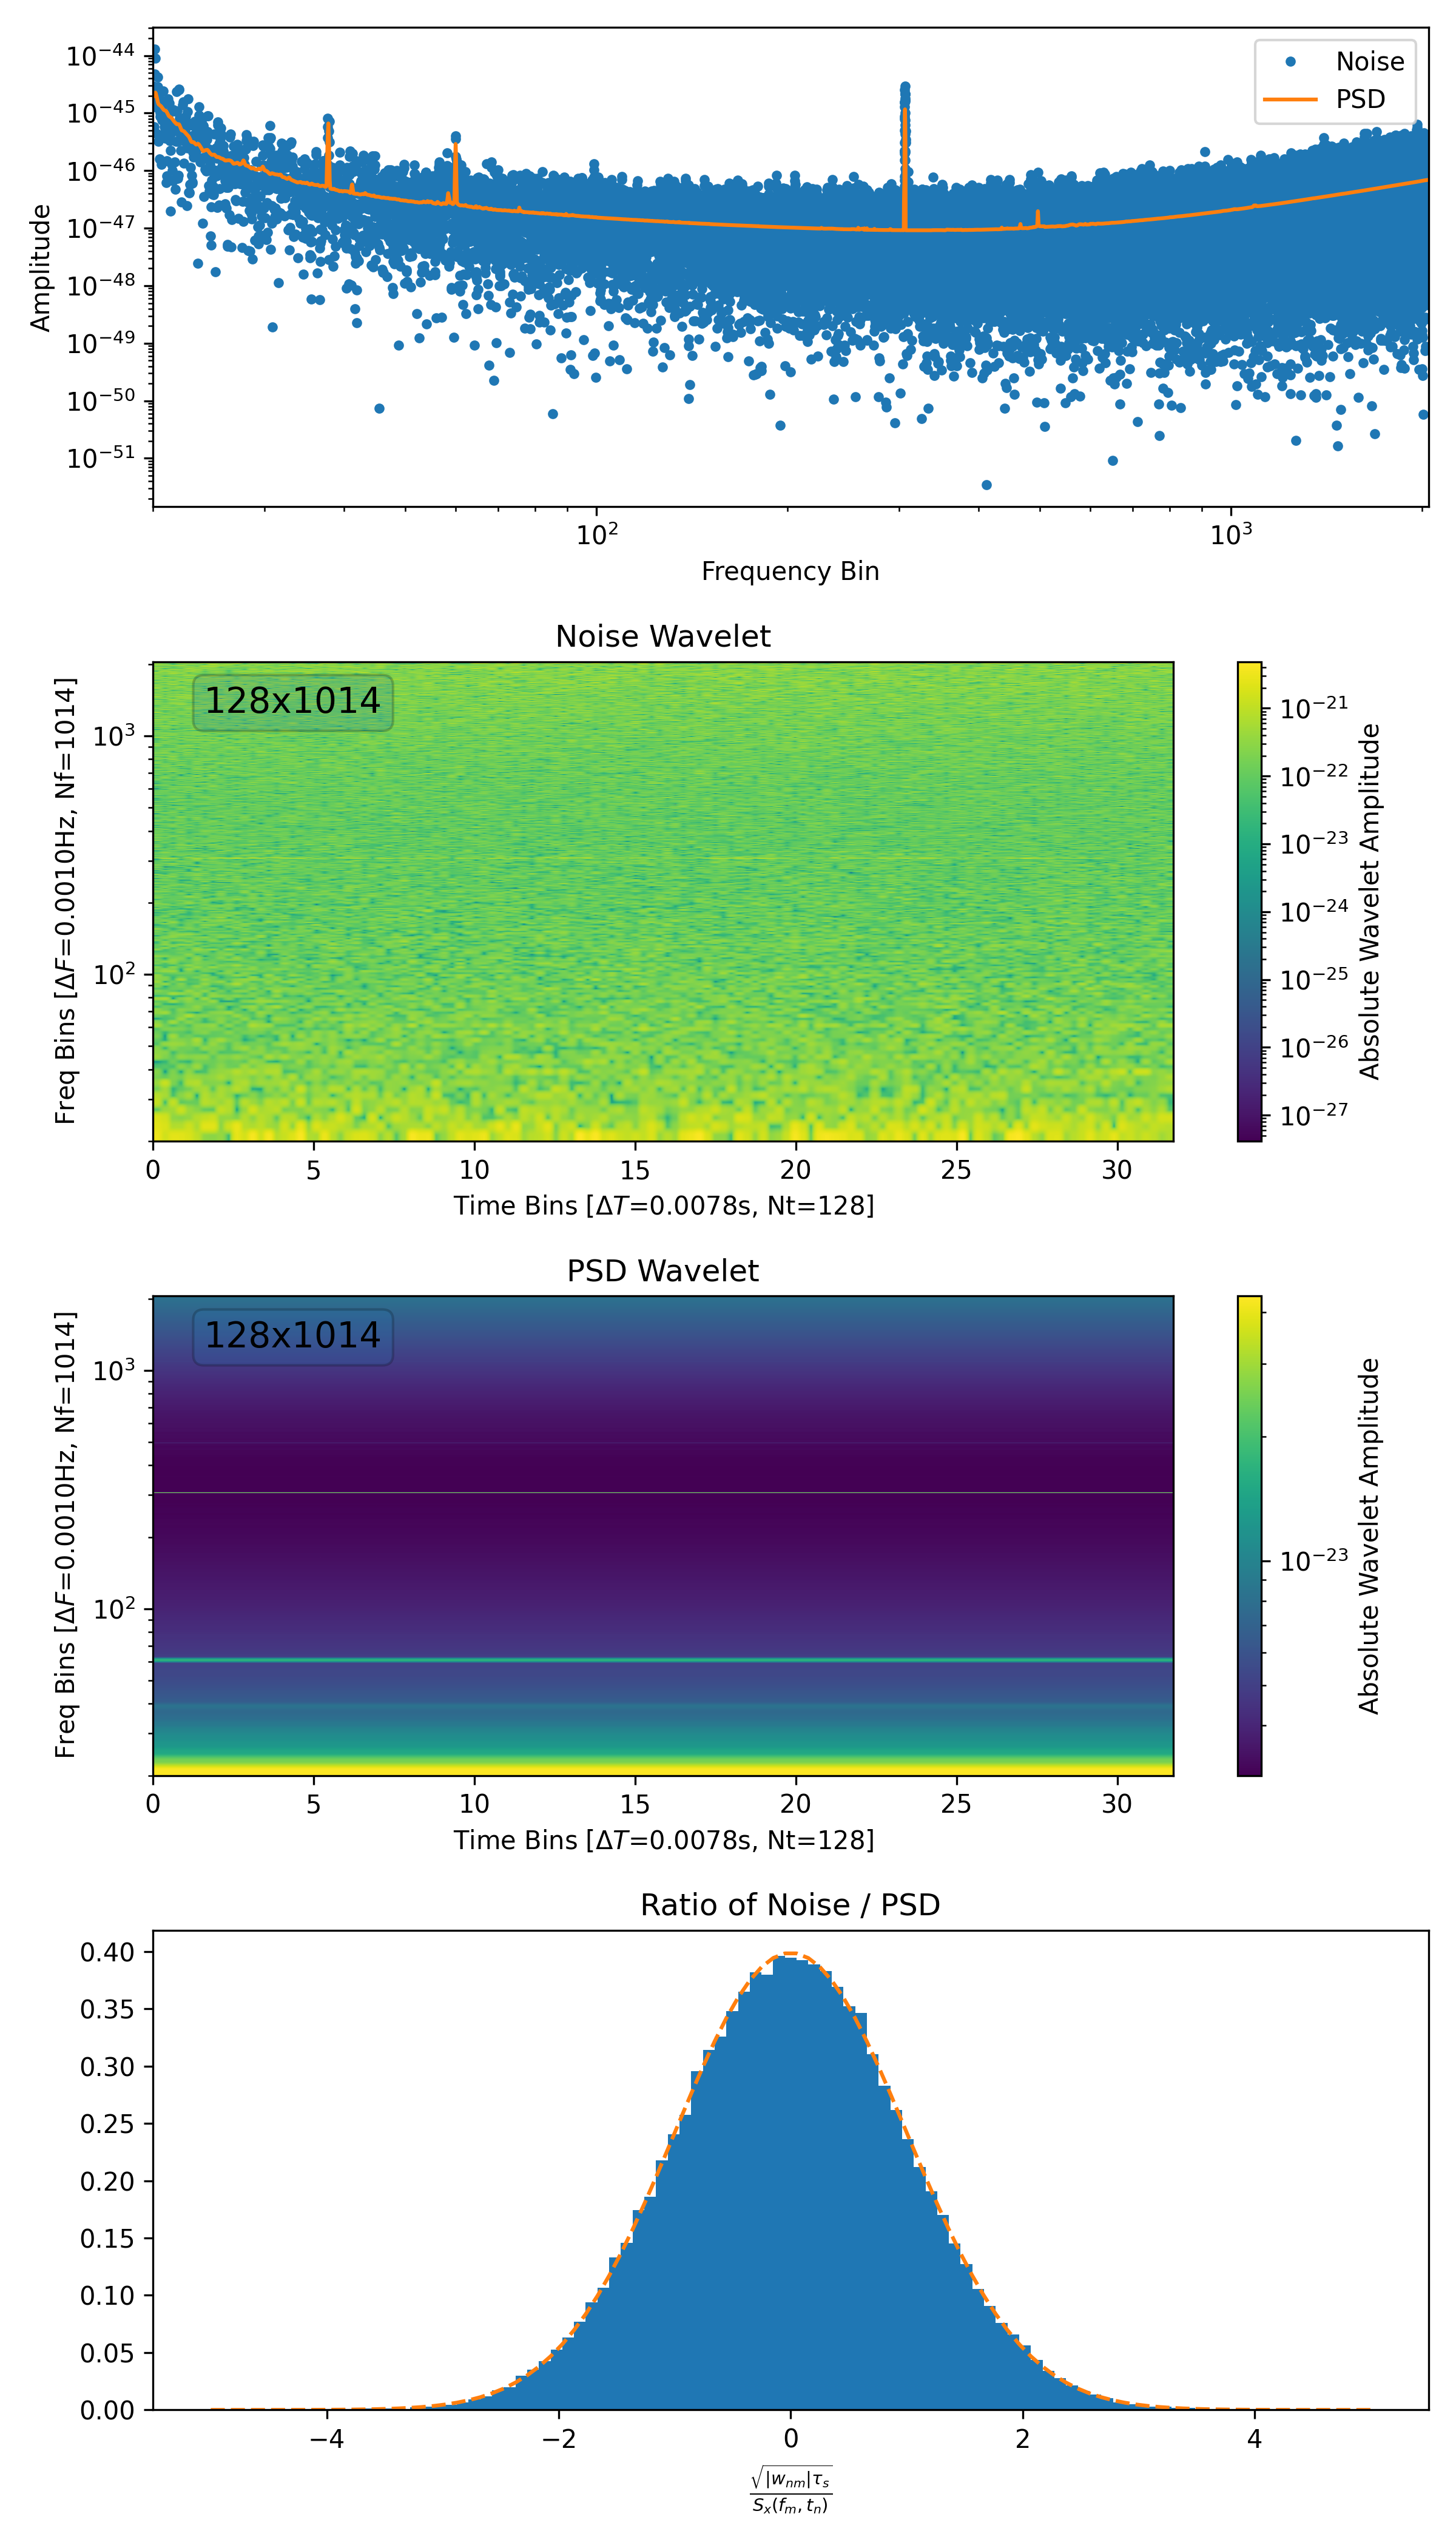
\includegraphics[width=\textwidth]{figures/PSD/lvk_wavelet_psd.png}
    \caption{$S_{\rm LVK}(f)\rightarrow n(\tau_n,f_m)$}
  \end{minipage}
  \hfill
  \begin{minipage}[b]{0.4\textwidth}
    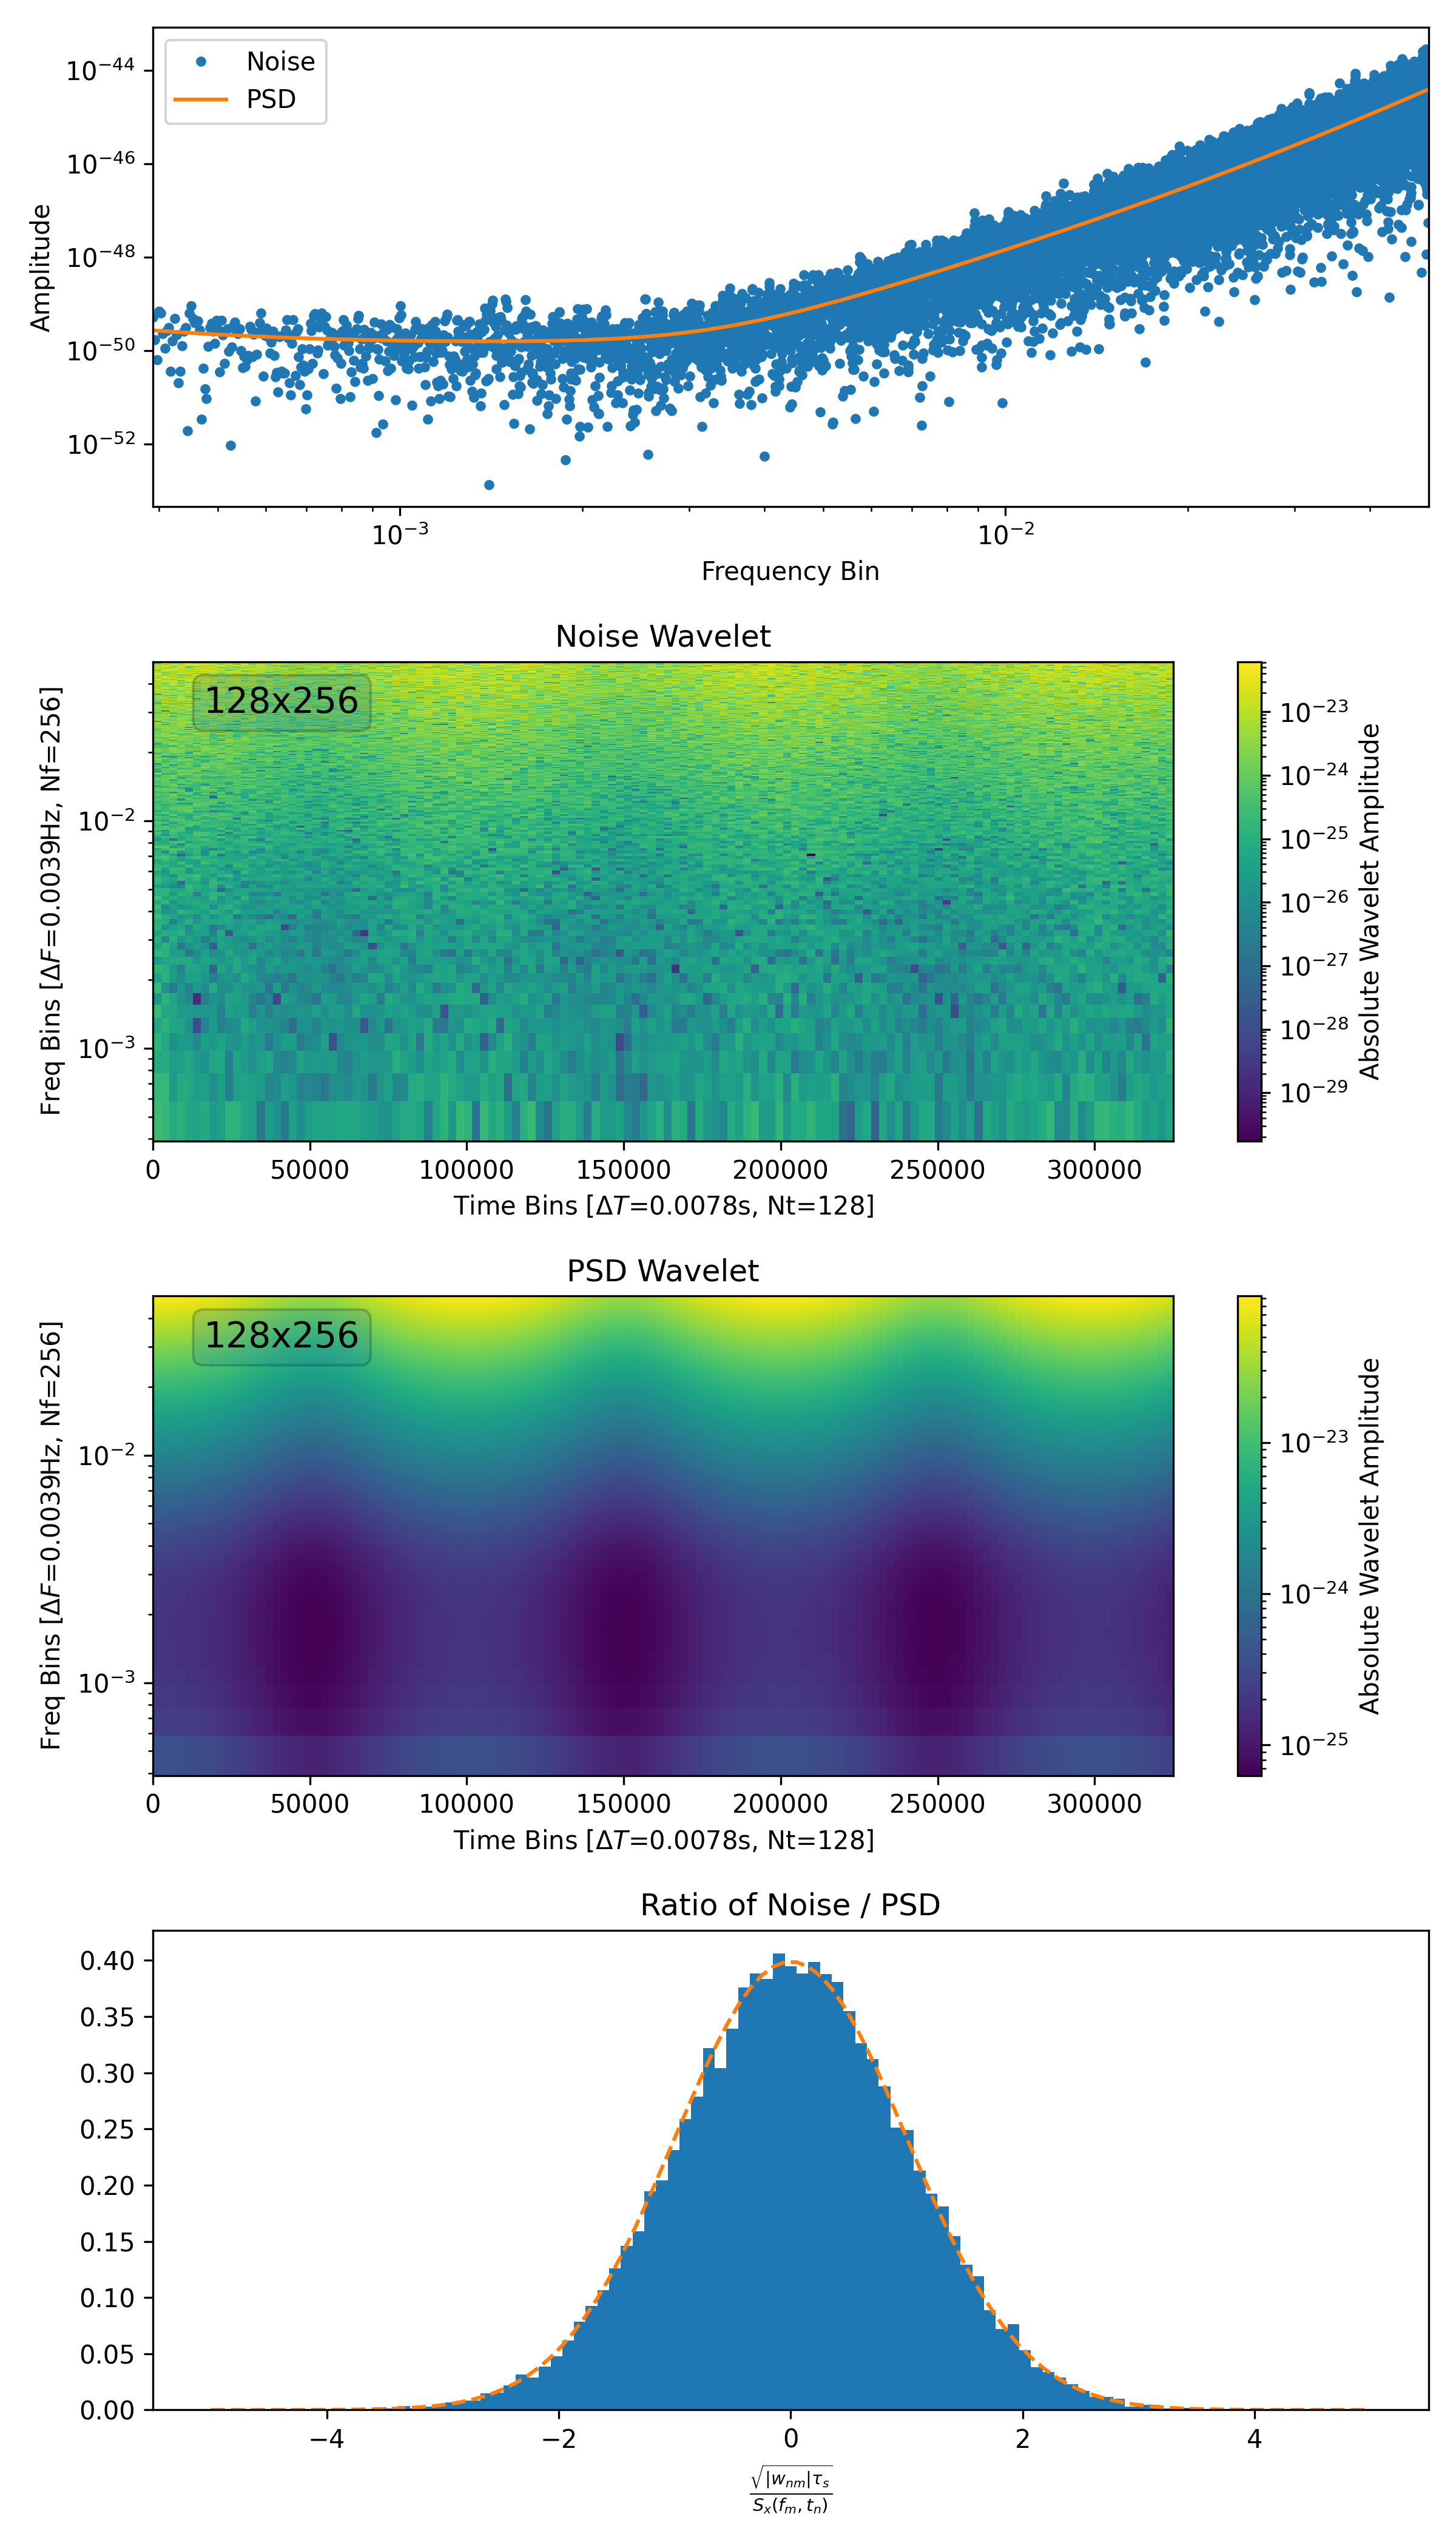
\includegraphics[width=\textwidth]{figures/PSD/lisa_wavelet_modulated_psd.png}
    \caption{$S_{\rm LISA}(f)*a(t)\rightarrow n(\tau_n,f_m)$}
  \end{minipage}
\end{figure}


For the non-stationary PSD, we multiply the stationary PSD $S_n(f)$ and with some time-varying function $g(t)$ leading to an amplitude-modulated spectrum $g(t)S_n(f)$. We can generate a timeseries from the $S_n(f)$, and then multiply the time series with the amplitude modulation ~\cite{nonstationary_psd}

% We now write the $g_{nm}$ as a function of their Fourier transform in the above expression:
% \begin{eqnarray}
%     W_{nm, n'm'} & = & \sum_{k=0}^{N-1} \sum_{k'=0}^{N-1} \int_{-\infty}^{+\infty} \int_{-\infty}^{+\infty} \tilde{g}_{nm}(f) \tilde{g}_{n'm'}(f') e^{2i\pi f k \tau_s} e^{-2i\pi f' k' \tau_s}  R(t_{k}, s_{k'}) \nonumber \\
%     & = & \int_{-\infty}^{+\infty} \int_{-\infty}^{+\infty} \tilde{g}_{nm}(f) \tilde{g}_{n'm'}(f') \sum_{k=0}^{N-1} \sum_{k'=0}^{N-1}   e^{2i\pi (f k - f'k')\tau_s} R(t_{k}, s_{k'}) 
% \end{eqnarray}


\subsection{Locally co-stationary time series}

Now we consider two time series $x$ and $y$ which are locally co-stationary and zero-mean. Let $w^{x}$ and $w_{y}$ be their wavelet transforms. We would like to estimate the covariance $\operatorname{E}[w^{x}_{nm}w^{y}_{n'm'}]$. We use a rationale similar as in Section~\ref{sec:locally_statioanry}.

\subsubsection{Definitions of autocorrelation and spectra}
Let us consider the time autocorrelation of $x$ and $y$ as
\begin{eqnarray}
    R_{xy}(t, s) = \operatorname{E}\left[x(t) y(s)\right].
\end{eqnarray}
We say that $x$ and $y$ are locally co-stationary processes if in the neighborhood of any point $\tau$ there exists an interval of size $l(\tau)$ and a length $d(\tau) < l(\tau)/2$ so that we have the relation \eqref{eq:locally-costationary} where we replace $R$ by $R_{xy}$, with similar definitions for $C_{xy}$ and the co-evolutionary spectrum $S_{xy}$.

\subsubsection{Wavelet cross-covariance}

We can associate a cross-covariance operator $T_{xy}$ to the cross autocovariance $R_{xy}$ and apply it to the wavelet basis:
Now, let us apply the covariance operator to the wavelet basis as
\begin{eqnarray}
\label{eq:cross-covariance-operator-applied-to-wavelet}
    \operatorname{T}_{xy}[g_{nm}](t) = \int_{-\infty}^{+\infty} R_{xy}(t, s) g_{nm}(s) ds
\end{eqnarray}
From the same arguments as in the previous section, we get 
\begin{eqnarray}
    \operatorname{T}_{xy}[g_{nm}](t) \approx \int_{-\infty}^{+\infty} S_{xy}(\tau_n, f) \tilde{g}_{nm}(f) e^{2i\pi f t}df
\end{eqnarray}
where $S_{xy}$ is the cross-evolutionary spectral density.
Based on the same approximation as for the wavelet covariance, we find that
\begin{eqnarray}
    \operatorname{T}_{xy}[g_{nm}](t) & \approx & S_{xy}^{\ast}(\tau_n, f_m)  \int_{-f_m -\Delta F}^{-f_m +\Delta F}\tilde{g}_{nm}(f) e^{2 i \pi f t}  df + S_{xy}(\tau_n, f_m)  \int_{f_m -\Delta F}^{f_m +\Delta F}\tilde{g}_{nm}(f) e^{2 i \pi f t}  df \nonumber
\end{eqnarray}
This time, the cross-spectral density $S_{xy}$ is a complex quantity.
Let us define
\begin{eqnarray}
    K_{nm}(t) \equiv \int_{f_m -\Delta F}^{f_m +\Delta F}\tilde{g}_{nm}(f) e^{2 i \pi f t}  df \approx \int_{0}^{+\infty}\tilde{g}_{nm}(f) e^{2 i \pi f t}  df 
\end{eqnarray}
so that we can write
\begin{eqnarray}
    \operatorname{T}_{xy}[g_{nm}](t) & \approx & S_{xy}^{\ast}(\tau_n, f_m)  K_{nm}^{\ast}(t) + S_{xy}(\tau_n, f_m)  K_{nm}(t) = 2 \Re\left\{ S_{xy}(\tau_n, f_m)  K_{nm}(t) \right\} \nonumber
\end{eqnarray}
The wavelet cross-covariance can then be developed as
\begin{eqnarray}
\label{eq:cross_cov_operator_property-applied}
\operatorname{E}\left[ \langle g_{nm} , x \rangle \langle g_{n'm'}, y \rangle^{\ast} \right]     & = & \frac{1}{\tau_s} \langle \operatorname{T}_{xy}[g_{nm}], g_{n'm'} \rangle \nonumber \\
    & = & \frac{1}{\tau_s} \sum_{k=0}^{N-1} \operatorname{T}_{xy}[g_{nm}](k \tau_s) g_{n'm'}(k \tau_s) \nonumber \\
    & = & \frac{1}{\tau_s} \sum_{k=0}^{N-1} \left( S_{xy}(\tau_n, f_m) K_{nm}[k] + S_{xy}(\tau_n, f_m)^{\ast} K_{nm}^{\ast}[k] \right) g_{n'm'}[k] \nonumber
\end{eqnarray}
By definition, we have $g_{n'm'} = K_{n'm'} + K_{n'm'}^{\ast}$. Let us inject this relation into the above equation:
\begin{eqnarray}
\label{eq:cross_cov_operator_property-applied-2}
\operatorname{E}\left[ \langle g_{nm} , x \rangle \langle g_{n'm'}, y \rangle^{\ast} \right]  
    & = & \frac{1}{\tau_s} \sum_{k=0}^{N-1} \left( S_{xy}(\tau_n, f_m) K_{nm}[k] + S_{xy}^{\ast} (\tau_n, f_m)K_{nm}^{\ast}[k] \right) \left(K_{n'm'}[k] + K_{n'm'}^{\ast}[k] \right)\nonumber \\
    & = & \frac{1}{\tau_s} \sum_{k=0}^{N-1} S_{xy}(\tau_n, f_m) \left( K_{nm}[k]K_{n'm'}[k] +  K_{nm}[k] K_{n'm'}^{\ast}[k] \right) \nonumber \\
    && + S_{xy}(\tau_n, f_m)^{\ast} \left( K_{nm}^{\ast}[k] K_{n'm'}[k] + K_{nm}^{\ast}[k] K_{n'm'}^{\ast}[k]\right)
    \nonumber \\
    &=& 2 \Re\left\{ \frac{1}{\tau_s} \sum_{k=0}^{N-1} S_{xy}(\tau_n, f_m) \left( K_{nm}[k]K_{n'm'}[k] +  K_{nm}[k] K_{n'm'}^{\ast}[k] \right) \right\}
\end{eqnarray}
We can compute the dot product $\lvert K_{nm} |  K_{n'm'} \rvert$:
\begin{eqnarray*}
    \lvert K_{nm} |  K_{n'm'} \rvert &=& \sum_{k=0}^{N-1} K_{nm}[k]K_{n'm'}[k] = \int_{0}^{+\infty}\int_{0}^{+\infty} \tilde{g}_{nm}(f) \tilde{g}_{n'm'}(f') \sum_{k=0}^{N-1}  e^{2i\pi (f + f') k \tau_s} df df'
\end{eqnarray*}
For large $N$, the quantity $\sum_{k=0}^{N-1}  e^{2i\pi (f + f') k \tau_s} \approx \delta(f+f')$ can be approximated by a delta Diract impulsion. Therefore
\begin{eqnarray*}
    \langle K_{nm} |  K_{n'm'} \rangle
    & \approx & \int_{0}^{+\infty}\int_{0}^{+\infty} \tilde{g}_{nm}(f) \tilde{g}_{n'm'}(-f) df \\
    & = & \int_{0}^{+\infty} e^{-i (n-n') 2 \pi f \Delta T} C_{n m} C_{n' m'}^{*} \tilde{\phi}(f-m \Delta F) \tilde{\phi}(-f+m' \Delta F)df
\end{eqnarray*}
where we ignored the terms that are negligible for positive frequencies. Since the function $\tilde{\phi}$ peaks at zero frequency, the above integral is non-zero (approximately) only if $m=m'$.
\begin{eqnarray*}
    \langle K_{nm} |  K_{n'm'} \rangle
    & \approx &  \delta_{m m'} \int_{0}^{+\infty} C_{n m} C_{n' m}^{*} | \tilde{\phi}(f-f_m) |^2 e^{-i (n-n') 2 \pi f \Delta T}  df \\
    & = & \int_{0}^{+\infty} C_{n m} C_{n' m}^{*} | \tilde{\phi}(f) |^2 e^{-i (n-n') 2 \pi (f+f_m) \Delta T}  df
\end{eqnarray*}
For $n = n'$, we get  
\begin{eqnarray*}
    \langle K_{nm} |  K_{n'm'} \rangle & = &  | C_{n m} |^2 \int_{0}^{+\infty}| \tilde{\phi}(f) |^2  df = \frac{1}{2},
\end{eqnarray*}
where we used the normalization of the window function $\int_{-\infty}^{+\infty}| \tilde{\phi}(f) |^2  df = 1$. For $n \neq n'$, we assume that the dot product is zero (we can actually prove it with the approximation $| \tilde{\phi}(f) |^2 \approx \frac{1}{2\Delta F} \Pi_{2\Delta F}(f)$). 

We just showed that $ \langle K_{nm} |  K_{n'm'} \rangle = \frac{1}{2}\delta_{nn'} \delta_{mm'}$. Using this result in Eq.~\eqref{eq:cross_cov_operator_property-applied-2}, we find that
\begin{eqnarray}
\label{eq:cross_cov_operator_property-applied-3}
\operatorname{E}\left[ \langle g_{nm} , x \rangle \langle g_{n'm'}, y \rangle^{\ast} \right]  
    &=& 2 \Re\left\{ \frac{1}{\tau_s}  S_{xy}(\tau_n, f_m) \right\}
\end{eqnarray}
\textcolor{purple}{Notice that this expression agrees with \eqref{eq:covariance_wnm} but not \eqref{eq:evolutionary_psd_delta_t}. We need to figure this out. This is of course only true if $S(\tau_{n},f_{m})\mathbb{R}$.}

% $| \tilde{\phi}(f) |^2 \approx \frac{1}{\Delta F} \Pi_{\Delta F}(f)$ so that
% \begin{eqnarray*}
%     \langle K_{nm} |  K_{n'm'} \rangle
%     & \approx &  \delta_{m m'} C_{n m} C_{n' m}^{*} \int_{-\Delta F/2}^{+\Delta F/2}  \frac{1}{\Delta F}e^{-i (n-n') 2 \pi (f+f_m) \Delta T}  df \\
%  & = & \delta_{m m'} C_{n m} C_{n' m}^{*} \frac{1}{\Delta F}
%     \left[ - \frac{1}{(n-n')2 i \pi \Delta T} e^{-i (n-n') 2 \pi (f + f_m) \Delta T}  \right]_{-\Delta F/2}^{+\Delta F/2} 
% \end{eqnarray*}
% \begin{eqnarray}
%     \operatorname{T}[g_{nm}](t) & \approx & 2 \Re \left\{ S(\tau_n, f_m)  \int_{f_m -\Delta F}^{f_m +\Delta F}\tilde{g}_{nm}(f) e^{2 i \pi f t}  df \right\} \nonumber \\
%     & = &  S(\tau_n, f_m) \int_{f_m -\Delta F}^{f_m +\Delta F} \left( \tilde{g}_{nm}(-f) e^{-2 i \pi f t}  df + S(\tau_n, f_m) \tilde{g}_{nm}(f) e^{2 i \pi f t} \right) df\nonumber \\
%     & = &  S(\tau_n, f_m) \int_{-\infty}^{+\infty} \tilde{g}_{nm}(f) e^{2 i \pi f t} df\nonumber \\
%     & = & S(\tau_n, f_m) g_{nm}(t)
% \end{eqnarray}

\section{Signal-to-noise Ratio}

In the wavelet domain, Cornish states the wavelet SNR is given by
\begin{equation}
    \rho(h) = \sum_{nm} \frac{\hat{h}_{nm}d_{nm}}{S_{nm}}
\end{equation}
Here we will define the optimal SNR must be:
\begin{equation}\label{eq:wavelet_domain_optimal_SNR}
    \rho(h) = \sum_{nm} \frac{h_{nm}h_{nm}}{S_{nm}}.
\end{equation}
In equation \eqref{eq:wavelet_domain_optimal_SNR}, the matrix $h_{nm}$ actually corresponds to the wavelet coefficients $\omega_{nm}$ that satisfy $\omega_{nm} = \sum_{nm}g_{nm}h[k]$ for $h$ the signal. The denominator is the evolutionary PSD, given by $S(t_{n},f_{m})$. The equation \eqref{eq:wavelet_domain_optimal_SNR} should be interpreted as a point-wise multiplication of the matrices with a sum over each element of $n$ and $m$. 

As an example, consider the monochromatic signal if \eqref{eq:simple_monochromatic_waveform} $h = A\sin(2\pi f_{0} t)$ for constants $A$ and $f_{0}$. We showed in section \ref{subsubsec:monchromatic_wavelet_calculations} that the wavelet coefficients had the form of  
\begin{equation}
\omega_{nm} = 
\begin{cases}
     0 & \text{if } n \in 2\mathbb{Z}_{\geq 0} \ \wedge \forall m\\
    A\sqrt{2 N_{f}} & n \in 2\mathbb{Z}_{\geq 0} + 1 \ \wedge  m = 2m_{0}/N_{t} \in 2\mathbb{Z}_{\geq 0}
\end{cases}
\end{equation}
In the expression above, there are precisely $N_{t}/2$ non-zero elements corresponding to the row elements governed by the index $m = 2m_{0}/N_{t}$. Keeping this in mind and substituting the expression for the wavelet coefficients in above, we find
\begin{align}\label{eq:SNR_monochromatic_source}
\rho^{2}_\text{wavelet} = \frac{A^{2} 2 N_{f} [N_{t}/2]}{S_{nm}} \approx \frac{A^{2} N_{f} N_{t}}{S(f_{0})/\Delta t} 
 = \frac{A^{2} N\Delta t}{S(f_{0})} 
 = \frac{A^2 T}{S(f_{0})}\,.
\end{align}
Where we have also used the approximation that $S(f_{m},t_{n}) = S(f_{m})/\Delta t$ for $S(f_{m})$ the usual one-sided power spectral density.

An independent calculation to verify \eqref{eq:SNR_monochromatic_source} can be reached using Parseval's theorem. Observe the usual noise-weighted inner product expressed in the frequency domain
\begin{equation}
(a|b) = 4\text{Re}\left(\int_{0}^{\infty}\frac{\tilde{a}^{\star}(f)\tilde{b}(f)}{S_{n}(f)}\,\text{d}f\right)\,,
\end{equation}
with $S_{n}(f)$ a one-sided power spectral density. The optimal matched filter SNR takes the form $\rho^2 = (h|h)$, i.e.,
\begin{equation}
(h|h) = 4\text{Re}\left(\int_{0}^{\infty}\frac{|\tilde{h}(f)|^2}{S_{n}(f)}\,\text{d}f\right)\,,
\end{equation}
Now, since $f_{0}$ is constant in $h = A\sin(2\pi f_{0}t)$, we can pull the PSD out and rewrite the above equation using Parseval's theorem.
\begin{align}
\rho_{\text{freq}}^2 = (h|h) = 4\text{Re}\left(\int_{0}^{\infty}\frac{|\tilde{h}(f)|^2}{S(f)}\,\text{d}f\right) = \frac{2}{S_{n}(f_{0})}\text{Re}\left(\int_{-\infty}^{\infty}|\tilde{h}(f)|^2\,\text{d}f\right) &= \frac{2}{S(f_{0})}\int_{0}^{T_{\text{obs}}}h(t)^2\,\text{d}t \\ 
&\approx \frac{A^2 T_{\text{obs}}}{S(f_{0})} \label{eq:SNR_monochromatic_signal_freq}
\end{align}
Where in the last step we wrote $h^2 = A^2\cos^2(2\pi f_{0} t) = A^2(1 - 2\cos(4\pi f_{0}t))/2$ and neglected the oscillatory piece for $T_{\text{obs}}\rightarrow \infty$. Notice that the SNR in the wavelet domain agreees with the SNR in the frequency domain, i.e., $\rho^2_{\text{freq}} = \rho^2 _{\text{wavelet}}$. This is comforting. 

We will define the wavelet inner product as follows
\begin{equation}
(a|b) = \sum_{nm}\frac{a_{nm}b_{nm}}{S_{nm}}.
\end{equation}




\newpage

\section{GW Data analysis}
\subsection{Wavelet-domain waveforms}
\avi{These are just my notes -- Ollie is now getting involved :) }

Waveform models such as \textsc{IMRPhenomXPHM}, \textsc{SEOBNRv4PHM} etc are defined in either the time or frequency domain. To analyse data in the wavelet domain, we need waveform models in the wavelet domain. We can do this by:
\begin{enumerate}
    \item Using the equations in Section~\ref{sec:wavelet_domain} to transform time/freq models during analysis. However, this conversion can be costly
    \item Using a surrogate wavelet representation of the waveforms in the wavelet domain.
\end{enumerate}

In the remainder of this section, we discuss two methods of building a surrogate wavelet representation of a waveform.

\subsubsection{Lookup Table wavelet model}
Cornish proposed several methods to obtain waveforms directly in the wavelet domain, and one was the \textit{lookup-table} method (Section VB, Fast Wavelet Waveforms: Taylor expansion). A GW waveform $h(t, \theta)$ can be written into its phase $\phi(t, \theta)$ and amplitude $A(t,\theta)$ components as 
\begin{align}
h(t;\theta)&=A(t,\theta)\ {\rm exp}[i\Phi(t,\theta)]\,\hspace{2em} {\rm or} \label{eq:ht}\\
\tilde{h}(f;\theta)&=A(f,\theta)\ {\rm exp}[i\tilde{\Phi}(f,\theta)]\,
\end{align}

We can first focus on the time-domain equation \eqref{eq:ht}. Taylor expanding the the phase $\Phi(t;\theta)$ and amplitude $A(t;\theta)$ about a specific wavelet time-bin $t=t_n = n\Delta T$ gives us:
\begin{alignat}{2}
    \Phi(t;\theta) = \Phi(t_{n} + (t - t_{n});\theta) &\approx \Phi(t_n;\theta) 
                     + \dot{\Phi}(t_n; \theta)\ (t - t_n) 
                     + \ddot{\Phi}(t_n; \theta)\ (t - t_n)^2/2
                     + \label{eq:phi_taylor_approx} \\
    A(t;\theta) = A(t_{n} + (t - t_{n});\theta) &\approx A(t_n;\theta) + \dot{A}(t_n;\theta)(t-t_n) + \ddot{A}(t_{n};\theta)(t-t_{n})^2/2        
\end{alignat}
Now, we can use the following relations \ob{explain this better}
\begin{alignat*}{2}
\dot{\Phi}(t) &= 2\pi f(t) ,\hspace{2em} \frac{\text{d}\Phi}{\text{d}f} &&= 2\pi t(f) \\
\ddot{\Phi}(t) &= 2\pi \dot{f}(t) ,\hspace{2em} \frac{\text{d}^{2}\Phi}{\text{d}f^{2}} &&= 2\pi t'(f) \\
\end{alignat*}

It is then possible to construct the wavelet coefficients via 
\begin{equation}
\omega_{nm} = A(t_{n})(c_{nm}(f_{n},\dot{f}_{n})\cos\Psi(t_{n}) + s_{nm}(f_{n},\dot{f}_{n})\sin\Psi(t_{n}))
\end{equation}
for
\begin{align}
c_{nm}(f,\dot{f}) &= \int \text{d}t\, g_{nm}(t)\cos(2\pi(t-t_{n})f + \pi(t-t_{n})^2\dot{f})\,, \\
s_{nm}(f,\dot{f})&= \int \text{d}t\,  g_{nm}(t)\sin(2\pi(t-t_{n})f + \pi(t-t_{n})^2\dot{f})\,.
\end{align}

\subsubsection{Time-domain example}
Consider chirping signal of the form
\begin{equation}
h = A\cos(2\pi f(t))\, \quad \ \text{with} \ f(t) = f_{0} + \dot{f}_{0}t \label{eq:lookup_chirp_example_signal}\,,
\end{equation}
For constants $A, f_{0}, \dot{f}_{0} \in \mathbb{R}$. We can put this into the form of $h = A\exp(i\Psi(t))$ by setting 
\begin{equation}
\Psi(t) = f_{0}t + \dot{f}_{0}t^2 / 2 
\end{equation}
where, for ease, we have set the integration constant to zero at $t = 0$. The phase here has an (exact) Taylor expansion of the form
\begin{align}
\Psi(t) &= \Psi(t_{n}) + \dot{\Psi}(t_{n})(t - t_{n}) + \ddot{\Psi}(t_{n})(t - t_{n})^2 / 2 \\
&= f_{0}t + \dot{f}_{0}t^2 / 2, \quad \ \text{after algebra, somewhat expected} 
\end{align}
Thus, in the discrete domain, the quantities $c_{nm}$ and $s_{nm}$ are given by 
\begin{align}
c_{nm}(f,\dot{f}) &\approx \Delta T\sum_{i = 0}^{N_{t}}g_{nm}(i\Delta T)\cos(2\pi([i - n]\Delta T)f + \pi([i - n]\Delta T)^2 \dot{f}) \\
s_{nm}(f,\dot{f}) &\approx \Delta T\sum_{i = 0}^{N_{t}}g_{nm}(i\Delta T)\sin(2\pi([i - n]\Delta T)f + \pi([i - n]\Delta T)^2 \dot{f})
\end{align}
We can then compute $c_{nm}(f,\dot{f})$ and $s_{nm}(f,\dot{f})$ on 2D grid for $\dot{f}$ and $\dot{f}$ and build a 2D interpolant. Once a table for $c_{nm}$ and $s_{nm}$ are built, the wavelet domain waveforms and be generated cheaply.  


% we can rewrite $\phi(t,\theta)$ from Eq~\ref{eq:phi_taylor_approx} as 
% \begin{alignat}{2}
%     \Phi(t,\theta) &= \Phi(t_n, \theta) \nonumber\\
%                    &  + 2\pi f(t_n, \theta)\ (t - t_n) \nonumber\\
%                    &  + \pi f'(t_n, \theta)\ (t - t_n)^2 \nonumber\\
%                    &  + ... \label{eq:phi_taylor_approx_2} 
% \end{alignat}

% Rewriting $h(t,\theta)$ Eq.~\ref{eq:ht} using the Taylor expansion (Eq~\ref{eq:phi_taylor_approx_2}) for $\Phi(t,\theta)$,
% \begin{align}
%     h(t,\theta) &= A(t,\theta)\ {\rm exp}[i\ \Phi(t, \theta)]\\
%                 &= A(t,\theta)\ {\rm exp}[i ( \Phi(t_n, \theta) + 2\pi f(t_n, \theta)\ (t - t_n) + \pi f'(t_n, \theta)\ (t - t_n)^2)]
% \end{align}
     





\subsubsection{Reduced order model:}
Reduced order modeling (ROM) speeds up waveform evaluation in GW astronomy~\cite{2022LRR....25....2T}. To build a reduced order waveform $h_{\rm ROM}(t, \vec{\theta})$, there are two stages:
\begin{enumerate}
    \item Obtaining $\{X_j\}^{Nx}$ `empirical interpolation nodes' (specific time or frequency nodes) for evaluation (the waveform is then generated by interpolating between all $\{X_j\}^{Nx}$).
    \item Generating a basis of waveforms $B=\{h(x,\vec{\theta}_i)\}^{Nb}$ that can be summed up with weights $w_i(t)$ to obtain any other waveform.
\end{enumerate}

The ROM for GW waveform can be given by $h_{\rm ROM}(t,\vec{\theta})=\rm{Interp}[h_{\rm ROM}(x,\vec{\theta})](t)$ can be written as:
\begin{equation}
    h(x,\vec{\theta}) \approx \sum^{\rm \#Basis}_i w_i(\theta) B_i(x)\ ,
\end{equation}
where $B_i(t)$ are the basis, eg $B = \{h(t, \vec{\theta})\}$), and $w_i(t)$ are projection coefficients (weights). The basis can be selected using a greedy approach (iteratively adding the waveform that most improves the overlap between the $h_{\rm ROM}$ and $h_{\rm True}$). Additionally, $w_i(t)$ can be fit using  polynomial interpolation, splines, radial basis, or ML
regression approaches.


In our case, our waveforms will be matrices:

\begin{equation}
    h(x,y,\vec{\theta}) \approx \sum^{\rm \#Basis}_i w_i(\theta) B_i(x,y)\ ,
\end{equation}







\subsection{Likelihood}
Given a time and frequency grid, the Whittle likelihood can be written as 
\begin{equation}
    \mathcal{L}(d|\theta) = -\frac{1}{2}\sum_{t_i,f_j}\left( {\rm ln}(2\pi S[t_i,f_j]) + \frac{(d[t_i,f_j] -h(\theta)[t_i,f_j])^2}{S[t_i,f_j]} \right)
\end{equation}
\avi{However, doesn't this assume that each gridpoint is independent?}


\begin{itemize}
    \item how do different time-freq grids affect the signals' SNR in the wavelet domain?
    \item Generate noise in time and wavelet transform it
    \item Compute the wavelet-SNR + the timeseries SNR
\end{itemize}




\subsection{`Dynamical' whittle likelihood}



\newpage

\section{Analytical derivation of a chirping signal in the wavelet domain}

\subsection{Discrete time-domain Taylor expansion (Giorgio)}

We would like to perform the analytical expression of a chirping signal as the ones used by \url{https://docs.scipy.org/doc/scipy/reference/generated/scipy.signal.chirp.html}, making a comparison with what has been obtained in \url{https://avivajpeyi.github.io/pywavelet/demos/roundtrip_demo.html}. In particular, we set the variable \textit{method='quadratic'}, which means that the signal, in time domain, will be (that's verified numerically)
\begin{align}\label{eq:h_t_cubic}
h(t)=\cos(2\pi\left[f_0t+(f_1-f_0)\frac{t^3}{3t_1^2}\right])
\end{align}
which can be discretized through $t=\frac{T}{N}k$, obtaining the following
\begin{align}\label{eq:h_k}
h[k]=\cos(2\pi\left[f_0\frac{T}{N}k+\frac{(f_1-f_0)}{3t_1^2}\frac{T^3}{N^3}k^3\right])
\end{align}
On the other hand, a good approximation of the Meyer filter is the rectangle function, whose discretized version in the time domain is
\begin{align}
\phi[k]=\textcolor{red}{\frac{1}{\sqrt{2\pi}}}\text{sinc}\left(\frac{\pi k}{2 N_f}\right)
\end{align}
where we remind that both formulas have $k=1\dots N$. Now, given the fact that we suppose the characteristic frequencies in the signal of \eqref{eq:h_k} vary slowly in time, a good approximation of \eqref{eq:h_k} is
\begin{align}
h[nN_f+k]&\simeq\cos(2\pi\varphi_0^n+2\pi\varphi_1^n k)\nonumber\\
\varphi_0^n&=\frac{f_0T}{N_t}n+\frac{f_1-f_0}{3t_1^2}\frac{T^3}{N_t^3}n^3\nonumber\\
\varphi_1^n&=\frac{f_0T}{N}+\frac{f_1-f_0}{t_1^2}\frac{T^3}{N_t^3N_f}n^2
\end{align}
And then using
\eqref{eq:direct} we obtain
\begin{align}
w_{n m}&=\sqrt{2} \frac{T}{N} \Re \left[C_{n m} \sum_{k=-qN_f}^{qN_f-1} e^{i \pi k m / N_f} h\left[n N_f+k\right] \phi[k]\right]=\nonumber\\
&=\sqrt{2} \frac{T}{N} \Re \left[C_{n m} \sum_{k=-qN_f}^{qN_f-1} e^{i \pi k m / N_f}\cos\left(2\pi\varphi_0^n+2\pi\varphi_1^n k\right)\frac{1}{\sqrt{2\pi}}\text{sinc}\left(\frac{\pi k}{2 N_f}\right)\right]=\nonumber\\
&=\frac{T}{N} \Re \left[C_{n m} \sum_{k=-qN_f}^{qN_f-1} e^{i \pi k m / N_f}\frac{e^{2\pi i\varphi_0^n+2\pi i\varphi_1^n k}+c.c.}{2}\frac{1}{\sqrt{\pi}}\frac{e^{i\frac{\pi k}{2 N_f}}-c.c.}{i\frac{\pi k}{N_f}}\right]=\nonumber\\
&=\frac{T}{N_t2\pi\sqrt{\pi}} \Im \left[C_{n m} \sum_{k=-qN_f}^{qN_f-1} e^{i \pi k m / N_f}\left(e^{2\pi i\varphi_0^n+2\pi i\varphi_1^n k}+c.c.\right)\frac{e^{i\frac{\pi k}{2 N_f}}-c.c.}{k}\right]=\nonumber\\
&= \frac{T}{N_t2\pi\sqrt{\pi}} \Im \Bigg[C_{n m} e^{2\pi i\varphi_0^n}\sum_{k=-qN_f}^{qN_f-1}\frac{1}{k}\left(e^{2\pi i\left(\varphi_1^n+\frac{1}{4N_f}+\frac{m}{2N_f}\right) k}-e^{2\pi i\left(\varphi_1^n-\frac{1}{4N_f}+\frac{m}{2N_f}\right) k}\right)+\nonumber\\
&+C_{n m} e^{-2\pi i\varphi_0^n}\sum_{k=-qN_f}^{qN_f-1}\frac{1}{k}\left(e^{2\pi i\left(-\varphi_1^n+\frac{1}{4N_f}+\frac{m}{2N_f}\right) k}-e^{2\pi i\left(-\varphi_1^n-\frac{1}{4N_f}+\frac{m}{2N_f}\right) k}\right)\Bigg]=\nonumber\\
&=\frac{T}{N_t2\pi\sqrt{\pi}} \Im \Bigg[C_{n m} \cos(2\pi\varphi_0^n)\frac{2\pi i}{N_f}
\end{align}
\textcolor{red}{Last equation is work in progress...}

\subsection{Continuous time-domain Taylor expansion (Quentin)}

\subsubsection{General case starting from Eq.~\eqref{wnm_def}}

Let us start from the general expression of the wavelet transform in Eq.~\eqref{wnm_def}:
\begin{equation*}
w_{nm}=\sum_{k=0}^{N-1}x[k]g_{nm}[k]
\end{equation*}
and the expression of $g_{nm}$ in the Fourier domain in Eq.~\eqref{eq:gnm}
\begin{equation*}
\tilde g_{mn}(f)=e^{-in f \Delta T} \tilde{h}_{nm}(f)
\end{equation*}
where we defined $\tilde{h}_{nm}(f) \equiv C_{nm}\tilde\phi(f-m\Delta F)+C^*_{nm}\tilde\phi(f+m\Delta F)$. Taking the inverse Fourier transform of the last equation yields
\begin{equation*}
g_{mn}(t)= h_{nm}(t - n \Delta T)
\end{equation*}
so that Eq.~\eqref{wnm_def} can be rewritten as a convolution:
\begin{eqnarray}
\label{eq:wnm-as-convolution}
w_{nm} = \sum_{k=0}^{N-1} x[k] h_{nm}(k \Delta t - n \Delta T) & \approx & \frac{1}{\Delta t} \int_{-\infty}^{+\infty} x(t) h_{nm}(t - n \Delta T) dt %\\
%& = & \frac{1}{\Delta t} \int_{-\infty}^{+\infty} x(t - n \Delta T) h_{nm}(t) dt \\
%& = & \frac{1}{\Delta t} \int_{-\infty}^{+\infty} x(n \Delta T - t) h_{nm}(-t) dt
\end{eqnarray}
%It is unclear to me that $h_{nm}(t)$ is symmetric...
Let us write the signal as
\begin{eqnarray}
\label{eq:time_waveform_amp_phase}
    x(t) = \Re\left\{A(t) e^{i \Psi(t)} \right\} = \frac{1}{2}A(t)\left(e^{i \Psi(t)} + e^{-i \Psi(t)}\right)
\end{eqnarray}
Let's assume that $A(t)$ evolves slowly with time, and let's Taylor-expand the phase:
\begin{eqnarray}
\label{eq:time_waveform_expansion}
    \Psi(t) \approx \Psi(t_n) + (t - t_n)\dot{\Psi}(t_n) + \frac{1}{2} (t-t_n)^2 \ddot{\Psi}(t_n)
\end{eqnarray}
where we wrote $t_n = n \Delta T$.
By plugging this Taylor expansion into Eq.~\eqref{eq:wnm-as-convolution}, we get
\begin{eqnarray}
\label{eq:wnm-as-convolution-taylor}
w_{nm} & \approx & \frac{1}{\Delta t} \Re \int_{-\infty}^{+\infty} A(t_n) e^{i\left(\Psi(t_n) + (t - t_n)\dot{\Psi}(t_n) + \frac{1}{2} (t-t_n)^2 \ddot{\Psi}(t_n) \right)} h_{nm}(t - t_n) dt \nonumber \\
& = & \frac{1}{\Delta t} \Re A(t_n) e^{i\Psi(t_n)}\int_{-\infty}^{+\infty} e^{i\left(t'\dot{\Psi}(t_n) + \frac{1}{2} {t'}^2 \ddot{\Psi}(t_n) \right)} h_{nm}(t') dt' \nonumber \\
& = & \frac{1}{\Delta t} \Re \left\{A(t_n) e^{i\Psi(t_n)} c_{nm}\right\}
\end{eqnarray}
where we used the change of variables $t'=t-t_n$ and we defined the following quantity:
\begin{eqnarray}
    c_{nm} & \equiv & \int_{-\infty}^{+\infty} e^{i\left(t'\dot{\Psi}(t_n) + \frac{1}{2} {t'}^2 \ddot{\Psi}(t_n) \right)} h_{nm}(t') dt'
\end{eqnarray}
We have:
\begin{eqnarray*}
    h_{nm}(t) &=& \int_{-\infty}^{+\infty} \left(C_{nm}\tilde\phi(f-m\Delta F)+C^*_{nm}\tilde\phi(f+m\Delta F) \right) e^{2i \pi f t} df \\
    &=& \int_{-\infty}^{+\infty} \tilde\phi(f') \left( C_{nm}e^{2i \pi (f'+f_m) t}+C^*_{nm} e^{2i \pi (f'-f_m)t } \right)  df' \\
    & = &  \int_{-\infty}^{+\infty} \tilde\phi(f')  e^{2i \pi f'} df' \left( C_{nm}e^{2i \pi f_m t}+C^*_{nm} e^{-2i \pi f_m t } \right)  \\
    & = & \phi(t) \left( C_{nm}e^{2i \pi f_m t}+C^*_{nm} e^{-2i \pi f_m t } \right)
\end{eqnarray*}
Consequently:
\begin{eqnarray*}
    c_{nm} & = & \int_{-\infty}^{+\infty} e^{i\left(t\dot{\Psi}(t_n) + \frac{1}{2} {t}^2 \ddot{\Psi}(t_n) \right)} \phi(t) \left( C_{nm}e^{2i \pi f_m t}+C^*_{nm} e^{-2i \pi f_m t }\right) dt \\
    & = & \int_{-\infty}^{+\infty} C_{nm}\phi(t) e^{i\left(t\dot{\Psi}(t_n) + \frac{1}{2} {t}^2 \ddot{\Psi}(t_n) \right)} e^{2i \pi f_m t } dt + \int_{-\infty}^{+\infty} C^\ast_{nm} \phi(t) e^{i\left(t\dot{\Psi}(t_n) + \frac{1}{2} {t}^2 \ddot{\Psi}(t_n) \right)} e^{-2i \pi f_m t } dt
\end{eqnarray*}
We define the instantaneous frequencies
\begin{eqnarray}
\label{eq:nu-def}
    \nu_n & \equiv & \frac{1}{2 \pi} \dot{\psi}(t_n) \\
    \dot{\nu}_n & \equiv & \frac{1}{2 \pi} \ddot{\psi}(t_n)
\end{eqnarray}
and the quantity 
\begin{equation}
\label{eq:zn-def}
\boxed{z_n(t) \equiv \phi(t) e^{i \pi t^2 \dot{\nu}_n}}
\end{equation}
The $c_{nm}$ can be re-written as a function of the Fourier transform of $z_n$:
\begin{equation}
\label{eq:cnm}
\boxed{
    c_{nm}  =  C_{nm} \tilde{z}_{n}\left(f_m + \nu_n\right) + C^\ast_{nm} \tilde{z}_{n}\left(f_m - \nu_n\right)
    }
\end{equation}
Eq.~\eqref{eq:cnm} requires to compute the Fourier transform of $z_{n}$, which can be expressed as a convolution:
\begin{equation}
    \tilde{z}_{n}(f) \equiv \int_{-\infty}^{+\infty} \tilde{\phi}(f') \tilde{u}(f-f') df'
\end{equation}
where we defined:
\begin{eqnarray}
  \tilde{u}(f) = \int_{-\infty}^{+\infty} e^{i \pi  t^2 \dot{\nu}(n\Delta T)} e^{-2 i \pi f t} dt = \frac{1}{\sqrt{\dot{\nu}(n\Delta T)}} e^{i \frac{\pi}{4}} e^{-i \frac{\pi f^2}{\dot{\nu}(n\Delta T)}}
\end{eqnarray}


\subsubsection{General case starting from Eq.~\eqref{eq:direct}}

% Combining the last two equations yield
% \begin{eqnarray*}
%     w_{nm} &=&\sum_{k=0}^{N-1} x[k] \int_{-\infty}^{+\infty} e^{-in f \Delta T} \tilde{h}_{nm}(f)e^{2 i \pi f k \Delta t} df  \\
%     &=& \int_{-\infty}^{+\infty} \tilde{h}_{nm}(f)  \sum_{k=0}^{N-1} x[k]e^{2 i \pi f (k \Delta t - n \Delta T)} df
% \end{eqnarray*}

Like Giogio above, we now start from Eq.~\eqref{eq:direct}:
\begin{equation}
w_{n m}=\sqrt{2} \Delta t \Re \left[C_{n m} \sum_{k=-K / 2}^{K / 2-1} e^{2\pi i k m q / K} x\left[n N_f+k\right] \phi[k]\right].
\end{equation}
where $K = 2q N_f$ is the width of the window function and $q$ determines the size of the window relative to the time resolution of the time-frequency pixels. This is equivalent to equation (13) of Cornish. In the code, they wrap the data $x$ to compute this sum.

Note that using the continuous approximation, the wavelet transform is essentially a convolution with the shifted window function:
\begin{eqnarray}
\label{eq:wavelet_transform_continuous}
    w_{n m} \approx \sqrt{2} \Re \left\{C_{n m} \int_{-\infty}^{+\infty} e^{2 \pi i t f_{m}} x(t_n + t) \phi(t) dt\right\},
\end{eqnarray}
where we set $t_n \equiv n \Delta T$ we use the following relations:
\begin{eqnarray}
  \Delta T &=& N_f \tau_s \label{eq:dT_tau}\\
  \frac{mq}{K}f_s &=& \frac{m}{2 N_f} f_s = m \Delta F = f_{m} \label{eq:fmq}
\end{eqnarray}
% Owing to the window function symmetry, we have equivalently:
% \begin{eqnarray}
% \label{eq:wavelet_transform_continuous_sym}
%     w_{n m} \approx \sqrt{2} \Re \left\{C_{n m} \int_{-\infty}^{+\infty} e^{-2 \pi i t f_{m}} x(t_n - t) \phi(t) dt\right\},
% \end{eqnarray}
We now use the expansion of the phase
\begin{eqnarray}
\label{eq:time_waveform_expansion2}
    \Psi(t_n + t) & \approx & \Psi(t_n) + t \dot{\Psi}(t_n) + \frac{1}{2} t^2 \ddot{\Psi}(t_n) \nonumber \\
    & = & \Psi(t_n) + 2 \pi t \nu_n + \pi t^2 \dot{\nu}_n
\end{eqnarray}
and then plug Eqs.~\eqref{eq:time_waveform_amp_phase} to get
\begin{eqnarray*}
    w_{n m} & \approx & \sqrt{2}A(t_n) \Re\Big\{ C_{n m}   \frac{1}{2} \int_{-\infty}^{+\infty} e^{2 \pi i t f_{m}} \left( e^{i\Psi(t_n)}  e^{i\left(2 \pi t \nu_n + \pi t^2 \dot{\nu}_n\right)} \right. \nonumber \\
    &&  \left. + e^{-i\Psi(t_n)} e^{-i\left(2 \pi t \nu_n + \pi t^2 \dot{\nu}_n\right)} \right)\phi(t)  dt \Big\}.
\end{eqnarray*}
Let us use the definition of $z_n$ in Eq.~\eqref{eq:zn-def}:
\begin{eqnarray*}
    w_{n m} & \approx & \sqrt{2}A(t_n) \Re\Big\{ C_{n m}   \frac{1}{2} \int_{-\infty}^{+\infty} e^{2 \pi i t f_{m}} \left( e^{i\Psi(t_n)+2 i\pi \nu_n t}  z_n(t) + e^{-i\Psi(t_n)-2 i\pi \nu_n t} z_n(t)^{\ast} \right)\phi(t)  dt \Big\}.
\end{eqnarray*}
The above expression can be expressed as Fourier transforms. Indeed, we have
\begin{eqnarray*}
    \int_{-\infty}^{+\infty} e^{2 \pi i t (f_{m}+\nu_n)} z_n(t) dt &=& \int_{-\infty}^{+\infty} e^{-2 \pi i t (f_{m}+\nu_n)} z_n(t) dt = \tilde{z}_n(f_{m} +\nu_n ) \\
    \int_{-\infty}^{+\infty} e^{2 \pi i t (f_{m}-\nu_n)} z_n(t)^{\ast} dt & = & \int_{-\infty}^{+\infty} e^{-2 \pi i t (f_{m}-\nu_n)} z_n(t)^{\ast} dt 
    = \tilde{z}^{\ast}_n(f_{m}-\nu_n)
\end{eqnarray*}
where we used the symmetry $z_n(-t) = z_n(t)$. Hence:
\begin{equation}
    \boxed{ w_{n m} \approx \sqrt{2} \frac{A(t_n)}{2}  \Re\Big\{ C_{n m} \left(  e^{i\Psi(t_n)}  \tilde{z}_n(f_{m} +\nu_n ) + e^{-i\Psi(t_n)} \tilde{z}^{\ast}_n(f_{m}-\nu_n)\right) \Big\}.}
\end{equation}

Another approach to the problem would be to keep using the discrete version of the wavelet transform in Eq.~\eqref{eq:direct} and perform the Taylor expansion:
\begin{eqnarray*}
w_{n m} & = & \sqrt{2} \Delta t \frac{A(t_n)}{2} \Re \left[C_{n m} \sum_{k=-K / 2}^{K / 2-1} e^{2\pi i k m q / K} \left( e^{i\Psi(t_n)+2 i\pi \nu_n k \Delta t}  z_n(k \Delta t) + e^{-i\Psi(t_n)-2 i\pi \nu_n k \Delta t} z^{\ast}_n(k \Delta t) \right) \phi[k]\right]
\end{eqnarray*}
where we recognise discrete Fourier transforms:
\begin{eqnarray*}
    \sum_{k=-K / 2}^{K / 2-1} e^{2 \pi i k (mq/K+\nu_n\Delta t)} z_n(k \Delta t) &=&  \sum_{k=0}^{K-1} e^{2 \pi i (k-K/2) (mq/K+\nu_n\Delta t)} z_n\left( (k-K/2) \Delta t \right) \\
    &=&  e^{- \pi i K (mq/K+\nu_n\Delta t)} \sum_{k=0}^{K-1} e^{2 \pi i k \frac{mq+\nu_n K \Delta t}{K}} z_n\left( (k-K/2) \Delta t \right) \\
    & = & e^{- \pi i K (mq/K+\nu_n\Delta t)} K \operatorname{IDFT}\left[z_n\left( (k-K/2) \Delta t \right)\right]\left(mq+\nu_n K \Delta t\right)
\end{eqnarray*}
where the DFT and IDFT operators are 
\begin{eqnarray}
    \operatorname{DFT}[z](w) & = & \sum_{k=0}^{K-1} z(k) e^{-2 i \pi \frac{wk}{K}} \nonumber \\
    \operatorname{IDFT}[z](u)  & = & \frac{1}{K} \sum_{k=0}^{K-1} z(k) e^{2 i \pi \frac{uk}{K}}
\end{eqnarray}
Similarly,
\begin{eqnarray*}
    \sum_{k=-K / 2}^{K / 2-1} e^{2 \pi i k (mq/K-\nu_n\Delta t)} z^{\ast}_n(k \Delta t) &=& \sum_{k=0}^{K-1} e^{2 \pi i (k-K/2) (mq/K-\nu_n\Delta t)} z_n^{\ast}\left((k-K/2) \Delta t\right) \\
    & = & e^{- \pi i K (mq/K-\nu_n\Delta t)} K \operatorname{IDFT}[z^{\ast}_n\left((k-K/2)\Delta t\right)](mq-\nu_n K \Delta t)
\end{eqnarray*}
By denoting $h_n(k) \equiv z_n\left( (k-K/2) \Delta t \right)$, we can write $w_{nm}$ as
\begin{eqnarray*}
w_{n m} & = & \sqrt{2} \Delta t \frac{A(t_n)}{2} \Re \left[C_{n m} e^{-\pi i m q }\left(e^{i\Psi(t_n)} e^{-i K \nu_n \Delta t } K \operatorname{IDFT}\left[z_n\right]\left(mq+\nu_n K \Delta t\right) \right. \right.\\
&& \left. \left. e^{-i\Psi(t_n)} e^{i K \nu_n \Delta t } K \operatorname{IDFT}^{\ast}\left[h^{\ast}_n\right](mq-\nu_n K \Delta t) \right) \right]
\end{eqnarray*}

%Then we can rewrite Eq.~\eqref{eq:wavelet_transform_continuous_expansion_2} as
% \begin{equation}
% \label{eq:wavelet_transform_continuous_expansion_3}
% \boxed{w_{n m}  \approx  \sqrt{2} A(t_n) \Re \left\{ C_{n m} \frac{1}{2} \left( e^{i\Psi(n\Delta T)} \tilde{c}_n\left(f_{m} - \nu(n\Delta T)\right) +  e^{-i\Psi(n\Delta T)} \tilde{c}_{n}^{\ast}\left(f_{m} + \nu(n\Delta T) \right) \right) \right\}}
% \end{equation}


% Note that if we ignore the second-order term, we get:
% \begin{eqnarray*}
% \label{eq:wavelet_time_approx_first_order}
%     w_{n m} & \approx & \sqrt{2}  A(t_n)  \Re \left\{ C_{n m} \frac{1}{2}\left[ e^{i\Psi(n\Delta T)} \tilde{\phi}\left( f_{m} - \nu(n\Delta T) \right) + e^{-i\Psi(n\Delta T)} \tilde{\phi}^{\ast}\left( f_{m} + \nu(n\Delta T) \right)\right]\right\}
% \end{eqnarray*}



% If we make the approximation that $\tilde{\phi}(f)$ is a rectangular window of width $\Delta F$ centered in $0$, i.e., $\tilde{\phi}(f) \approx \Pi_{\Delta F}(f) / \sqrt{\Delta F}$, we get:
% \begin{eqnarray*}
%     \tilde{c}_{n}(f) & \equiv & \frac{1}{\sqrt{\Delta F}} \int_{-\Delta F/2}^{+\Delta F / 2}  \tilde{u}(f-f') df' = \frac{1}{\sqrt{\Delta F}}\int_{f-\Delta F/2}^{f+\Delta F / 2}  \tilde{u}(\xi) d\xi \\
%     & = &  \frac{1}{\sqrt{\Delta F \dot{\nu}_{n}}}\left[U_{n}\left(f + \frac{\Delta F}{2}\right) - U_{n}\left(f - \frac{\Delta F}{2}\right)\right] 
% \end{eqnarray*}
% where we defined
% \begin{eqnarray*}
%     U_{n}(x) \equiv - \frac{\dot{\nu}_n}{2}\operatorname{erf}\left(e^{\frac{i \pi}{4}} \sqrt{\frac{\pi}{\dot{\nu}_n}} x\right)
% \end{eqnarray*}
% and $\dot{\nu}_n = \dot{\nu}(n \Delta T)$.

\subsubsection{Example of a chirp}
Let us consider the signal:
\begin{equation}
    x(t) = \cos\left( 2 \pi f_0 t + a t^{2} \right).
\end{equation}
for which we have 
\begin{eqnarray*}
    \Psi(t) & = & 2 \pi f_0 t + a t^{2} \nonumber \\
    \nu(t) & = & \frac{1}{2\pi} \dot{\Psi}(t) = f_0 + \frac{a t}{\pi} \nonumber \\
    \dot{\nu}(t) & = & \frac{a}{\pi}
\end{eqnarray*}
In this specific case, $\dot{\nu}(t)$ does not depend on time, therefore $\dot{\nu}_{n}$ does not depend on $n$. We can therefore compute $c_n$ once for all:
\begin{equation*}
z_{n}(t) \equiv \phi(t) e^{i a  t^2}
\end{equation*}

\subsubsection{The $t^3$ chirp (Giorgio)}
We start from \eqref{eq:wavelet_time_approx_first_order} and \eqref{eq:h_t_cubic} where now
%
\begin{align}
    \Psi(t) &= 2 \pi f_0 t + a t^{3}\nonumber\\
    \nu(t) &= f_0 + \frac{3 a}{2\pi} t^2\nonumber\\
    a&=2\pi \frac{f_1-f_0}{3t_1^2}
\end{align}
%
obtaining
%
\begin{align}
\label{eq:wavelet_time_approx_first_order_tcube}
w_{n m} \approx \sqrt{2} \Delta t \Re C_{n m} \frac{1}{2} A(t_n) e^{i\Psi(n\Delta T)} \tilde{\phi}\left( f_{mq} - f_0 - \frac{3a t_n^2}{2\pi} \right)
\end{align}

\subsection{Frequency-domain Taylor expansion}

Let us consider an arbitrary function of time $x(t)$ whose Fourier transform is $X(f)$.

The expression of the wavelet transform of $x$ involves the expression of $x_m$ in Eq.~\ref{eq:wdft}, whose continuous version can be expressed as
\begin{align}
\label{eq:wdft-continuous}
    x(f_m, \tau_n) = \int_{-\infty}^{+\infty} e^{-2\pi i f \tau_n} X(f+ f_m)\tilde{\phi}(f) df,
\end{align}
where we set $f_m = m N_t/2 f_s$ and $\tau_n = n \tau_s$.
The frequency window $\tilde{\phi}(f)$ represented in Fig.~\ref{fig:phi_omega} restricts the frequencies contributing to the integral to the bandwidth $\Delta F$ around the central frequency. 
The frequency-domain waveform can be split in amplitude and phase:
\begin{eqnarray}
\label{eq:amplitude_phase_split}
    X(f) = A(f) e^{i\Theta(f)}
\end{eqnarray}
Therefore, we can Taylor expand both amplitude and phase:
\begin{eqnarray}
    A(f + f_m) &=& A(f_m) + f A'(f_m) + ... \\
    \Theta(f + f_m) &=& \Theta(f_m) + f \Theta'(f_m) + \frac{1}{2} f^2 \Theta''(f_m)
\end{eqnarray}
Plugging this approximation into Eq.~\eqref{eq:wdft-continuous} yields
\begin{align}
\label{eq:wdft-continuous-taylor}
    x(f_m, \tau_n) & = \int_{-\infty}^{+\infty} e^{-2\pi i f \tau_n} \tilde{\phi}(f) A(f_m) e^{i \left(\Theta(f_m) + f \Theta'(f_m) + \frac{1}{2} f^2 \Theta''(f_m)\right)} df \nonumber \\
    & + \int_{-\infty}^{+\infty} e^{-2\pi i f \tau_n} \tilde{\phi}(f) \textcolor{red}{f} A'(f_m) e^{i\left(\Theta(f_m) + f \Theta'(f_m) + \frac{1}{2} f^2 \Theta''(f_m)\right)} df
\end{align}
For now, we will keep only the leading order in amplitude and concentrate on the phase expansion. We can take some terms out of the integral.
\begin{align}
\label{eq:wdft-continuous-taylor-2}
    x(f_m, \tau_n) & = A(f_m) e^{i\Theta(f_m)} \int_{-\infty}^{+\infty} \tilde{\phi}(f) e^{\frac{i}{2} f^2 \Theta''(f_m)} e^{2i \pi f \left( \frac{1}{2\pi}\Theta'(f_m) -  \tau_n\right)} df 
\end{align}
which is expressed as the inverse Fourier transform of the function $\tilde{z}(f) = \tilde{\phi}(f) e^{\frac{i}{2} f^2 \Theta''(f_m)}$.
%which is amazing as it shows we can construct wavelet templates from frequency-domain waveforms and their derivatives. 
Of course, we can extend this decomposition to arbitrary precision. 

% \subsubsection{Numerical approach}

% From Eq.~\eqref{eq:wdft-continuous-taylor-2} we see that computing the wavelet coefficients requires valuating quantities depending on the frequency phase derivatives:
% \begin{eqnarray}
% \label{eq:definition_enm}
% e_{nm} \equiv \int_{-\infty}^{+\infty} \tilde{\phi}(f)  e^{-2\pi i f \tau_n} e^{i \left(f \Theta'(f_m) + \frac{1}{2} f^2 \Theta''(f_m)\right)} df.
% \end{eqnarray}
% Let's approximate them with a discrete Fourier transform:
% \begin{eqnarray}
% e_{nm} \approx \frac{f_s}{N_t}\sum_{k=0}^{N_t-1} \tilde{\phi}(f_k)  e^{-2\pi i k n / N_t} e^{i \left(f_k \Theta'(f_m) + \frac{1}{2} f_k^2 \Theta''(f_m)\right)}.
% \end{eqnarray}
% where $f_k = k f_s / N_t$ are the Fourier frequencies corresponding to the wavelet time grid.
% This way, we can use the fast Fourier transform algorithm to comptue the DFT of 
% \begin{eqnarray}
%     \tilde{e}_{nm}(k) \equiv \tilde{\phi}(f_k) e^{i \left(f_k \Theta'(f_m) + \frac{1}{2} f_k^2 \Theta''(f_m)\right)}.
% \end{eqnarray}

Cornish argues that one can use the stationary phase approximation, where there is a map between time and frequency as:
\begin{eqnarray}
    f & \longrightarrow & t(f) = \frac{1}{2 \pi} \frac{d\Theta(f)}{df} \\
    t & \longrightarrow & f(t) = \frac{1}{2 \pi} \frac{d\Psi(t)}{dt} 
\end{eqnarray}

Let us define the function
\begin{eqnarray}
    \tilde{z}(f) \equiv \tilde{\phi}(f) e^{\frac{i}{2} f^2 \Theta''(f_m)}
\end{eqnarray}
Then the equation \eqref{eq:wdft-continuous-taylor-2} can be written as a function of the inverse Fourier transform of $\tilde{z}(f)$, that we label as $z(t)$:
\begin{align}
\label{eq:wdft-continuous-taylor-3}
    x(f_m, \tau_n) & = A(f_m) e^{i\Theta(f_m)} z\left(\tau_n - t(f_m) \right),
\end{align}
where we used 
\begin{eqnarray}
\label{eq:z_inverse_fourier}
    z(t) = \int_{-\infty}^{+\infty}\tilde{z}(f) e^{-2\pi i f t} df.
\end{eqnarray}
and $\Theta'(f) = 2 \pi t(f)$.

\subsubsection{First-order}
It is interesting to note that up to first order in the phase, we get

\begin{align}
\label{eq:wdft-continuous-taylor-first-order}
    x(f_m, \tau_n) \approx X(f_m) \phi\left(\tau_n - t(f_m) \right).
\end{align}

\subsubsection{Second-order}

To simplify the computation, we consider that the window function $\tilde{\phi}(f)$ is approximately rectangular so that
\begin{align}
\label{eq:meyer_window_freq_approx}
\tilde\phi(\omega) \approx \left\{\begin{array}{lr}
\frac{1}{\sqrt{2 \pi \Delta F }} & |f| < \frac{\Delta F}{2}\\
0 & \text{otherwise.}
\end{array}\right.\;,
\end{align}
Then the integral in Eq.~\eqref{eq:z_inverse_fourier} can be approximated as
\begin{align}
\label{eq:z_inverse_fourier-2}
    z(t) & = \frac{1}{\sqrt{2 \pi \Delta F }} \int_{-\Delta F/2}^{+\Delta F/2} e^{i\frac{1}{2} f^2 \Theta''(f_m)} e^{-2\pi i f t} df
\end{align}
 With Mathematica, we derive that 
\begin{eqnarray}
    z(t) & = & \frac{1}{\sqrt{2 \pi \Delta F }} \left[I_{\frac{\Delta F}{2}}(t) - I_{-\frac{\Delta F}{2}}(t)  \right] 
\end{eqnarray}
with
\begin{eqnarray}
    I_{T}(t) & = & -\frac{1}{2} \sqrt{\frac{\pi}{a}} e^{i\frac{3 \pi}{4} - i \frac{\pi^2 t^2}{a}} \operatorname{erfi}\left( e^{i\frac{\pi}{4}} \frac{aT - \pi t}{\sqrt{a}}\right)
\end{eqnarray}
where $\operatorname{erfi}$ is the imaginary error function and $a = \frac{1}{2} \Theta''(f_m)$.
Hence
\begin{align}%
\label{eq:wdft-continuous-taylor-second-order}
    x(f_m, \tau_n) \approx A(f_m) e^{i\Theta(f_m)} \frac{1}{\sqrt{2 \pi \Delta F }} \left[I_{\frac{\Delta F}{2}}(\tau_n - t(f_m)) - I_{-\frac{\Delta F}{2}}(\tau_n - t(f_m))  \right] 
\end{align}

Then, we simply need to apply Eq.~\eqref{eq:fast}:
\begin{align}
\label{eq:fast-2}
    w_{nm} & =\sqrt{2}(-1)^{nm}\Re\left[C_{nm} x(f_m, \tau_n)\right] \nonumber \\
\end{align}

\subsubsection{Example of a chirp}
Let us assume that the analysed signal is a chirp of the form 

\begin{equation}
\label{eq:chirp-time}
    x(t) = \cos\left( 2 \pi f_0 t + a t^{2} \right).
\end{equation}
We can decompose it as 
\begin{equation}
\label{eq:chirp-time-decomposed}
    x(t) = \cos\left( 2 \pi f_0 t \right) \cos\left(a t^{2} \right) - \sin\left( 2 \pi f_0 t \right) \sin\left(a t^{2} \right).
\end{equation}
The Fourier transform of the quadratic terms are 
\begin{eqnarray}
   \tilde{c}_{2}(f) \equiv \mathcal{F}\left[\cos\left(a t^{2} \right)\right](f) & =&  \sqrt{\frac{\pi}{a}} \cos\left(\frac{\pi^2 f^2}{a} - \frac{\pi}{4} \right) \nonumber \\
   \tilde{s}_{2}(f) \equiv \mathcal{F}\left[\sin\left(a t^{2} \right)\right](f) & =&  - \sqrt{\frac{\pi}{a}} \sin\left(\frac{\pi^2 f^2}{a} - \frac{\pi}{4} \right) 
\end{eqnarray}
So we can write the Fourier transform of \eqref{eq:chirp-time-decomposed} as
\begin{eqnarray}
    X(f) & = & \frac{1}{2}\left(\tilde{c}_{2}(f-f_0) + \tilde{c}_{2}(f+f_0)\right) - \frac{1}{2i}\left(\tilde{s}_{2}(f-f_0) - \tilde{s}_{2}(f+f_0)\right) \nonumber \\
    & = & \frac{1}{2}\left(\tilde{e}(f-f_0) + \tilde{e}(f+f_0)^{\ast}\right)
\end{eqnarray}
where we defined
\begin{eqnarray}
    \tilde{e}(f) & \equiv & \tilde{c}(f) + i \tilde{s}(f) = \sqrt{\frac{\pi}{a}} e^{-i \left(\frac{\pi^2 f^2}{a} - \frac{\pi}{4} \right)}
\end{eqnarray}
Therefore,
\begin{eqnarray*}
   X(f) &=& \frac{1}{2} \sqrt{\frac{\pi}{a}}  \left(e^{\frac{i\pi}{4}}  e^{-i\frac{\pi^2 (f-f_0)^2}{a}} + e^{-\frac{i\pi}{4}}  e^{i\frac{\pi^2 (f+f_0)^2}{a}} \right) \\
  & = &  \sqrt{\frac{\pi}{a}}  e^{2 i \frac{\pi^2 f_0 f }{a}} \cos\left(\frac{\pi^2}{a} (f^2 + f_0^2) - \frac{\pi}{4}\right) 
\end{eqnarray*}

Let us concentrate on the positive frequency part. By identification with Eq.~\eqref{eq:amplitude_phase_split}, we have
\begin{eqnarray}
    A(f) & = & \sqrt{\frac{\pi}{a}} \cos\left(\frac{\pi^2}{a} (f^2 + f_0^2)\right)  \nonumber \\
    \Theta(f) & = & \frac{2 \pi^2 f f_0}{a} - \frac{\pi}{4} \nonumber \\
    \Theta'(f) & = & \frac{2 \pi^2 f_0}{a}
\end{eqnarray}
Therefore, we have $t(f) = \frac{\pi f_0 }{a}$ and the first-order approximation of the wavelet coefficient is 
\begin{align}
\label{eq:chirp-first-order}
    w_{nm} & =\sqrt{2}(-1)^{nm}\Re\left[C_{nm} A(f_m)e^{i\Theta(f_m)} \phi\left(\tau_n - t(f_m) \right).\right] \nonumber \\
\end{align}

\section{GW detector response in the wavelet domain}

Here we examine the possibility of performing template-free GW searches in LISA data.

\subsection{As a function of the wavelet-domain GW waveform}
The detector's response to an incoming gravitational wave depends on its location in the sky, or equivalently, on its wave vector $\hat{\mathbf{k}}$. In LISA, it also depends on time (as the constellation moves around the Sun during the observation) and on the source's frequency. The link response to a particular polarization $p$ is therefore written as a convolution 
\begin{eqnarray}
y_{l m, p}(t, \hat{\mathbf{k}}) \approx & \frac{1}{2\left(1-\hat{\mathbf{k}} \cdot \hat{\mathbf{n}}_{l m}(t)\right)}\left[ 
 h_p\left(t-\frac{L_{l m}(t)}{c}-\frac{\hat{\mathbf{k}} \cdot \mathbf{x}_m(t)}{c}, \hat{\mathbf{n}}_k\right) 
-h_p\left(t-\frac{\hat{\mathbf{k}} \cdot \mathbf{x}_l(t)}{c}, \hat{\mathbf{n}}_k\right)\right] \xi_p\left(\hat{\mathbf{u}}_k, \hat{\mathbf{v}}_k, \hat{\mathbf{n}}_{l m}\right) .
\end{eqnarray}
where $h_p$ in the wave strain amplitude for polarization $p$ and $\xi_p$ are the modulation functions of the antenna pattern.
Let's set 
\begin{eqnarray}
    F_{lm, p}(t, \hat{\mathbf{k}}) & \equiv & \frac{1}{2\left(1-\hat{\mathbf{k}} \cdot \hat{\mathbf{n}}_{l m}(t)\right)} \xi_p\left(\hat{\mathbf{u}}_k, \hat{\mathbf{v}}_k, \hat{\mathbf{n}}_{l m}\right) \\ 
    \tau^{r}_{lm}(t, \hat{\mathbf{k}}) & \equiv & \frac{L_{l m}(t)}{c}-\frac{\hat{\mathbf{k}} \cdot \mathbf{x}_m(t)}{c}\\
    \tau^{e}_{lm}(t, \hat{\mathbf{k}}) & \equiv & \frac{\hat{\mathbf{k}} \cdot \mathbf{x}_l(t)}{c}.
\end{eqnarray}
For now, let us drop the link indices $l, m$ and polarization $p$ indices for clarity.
For each link and polarization, we thus have
\begin{eqnarray}
\label{eq:response_simple}
y(t, \hat{\mathbf{k}}) \approx & F(t, \hat{\mathbf{k}}) \cdot \left[ 
 h\left(t-\tau^{r}(t), \hat{\mathbf{k}}\right) -h\left(t-\tau^{e}(t), \hat{\mathbf{k}} \right) \right].
\end{eqnarray}
Now, we can decompose the time-domain GW perturbation in the wavelet basis, from Eq.~\eqref{eq:inverse_wavelet_decomposition}
\begin{align}
\label{eq:inverse_wavelet_decomposition_2}
h(t_k) = \sum_{n=0}^{N_t-1}\sum_{m=0}^{N_f-1}h_{nm}g_{nm}(t_k).
\end{align}
Let's first plug this expression into Eq.~\eqref{eq:response_simple}
\begin{eqnarray}
\label{eq:response_simple_decomp}
y(t, \hat{\mathbf{k}}) \approx & F(t, \hat{\mathbf{k}}) \sum_{n'=0}^{N_t-1}\sum_{m'=0}^{N_f-1}h_{n'm'}(\hat{\mathbf{k}}) \left[ 
 g_{n'm'}\left(t-\tau^{r}(t)\right) -g_{n'm'}\left(t-\tau^{e}(t))\right) \right].
\end{eqnarray}
Transforming the response into the wavelet domain gives
\begin{align}
\label{response_wavelet}
W[y]_{nm} & = \sum_{k=0}^{N-1} g_{nm}(t_k) y(t_k, \hat{\mathbf{k}}) \nonumber \\
& =  \sum_{n'=0}^{N_t-1}\sum_{m'=0}^{N_f-1}h_{n'm'}(\hat{\mathbf{k}}) \sum_{k=0}^{N-1}  g_{nm}(t_k)  F(t_k, \hat{\mathbf{k}})  \left[ 
 g_{n'm'}\left(t_k-\tau^{r}(t_k)\right) -g_{n'm'}\left(t_k-\tau^{e}(t_k))\right) \right]
\end{align}
Let us define the kernel
\begin{eqnarray}
\label{eq:kernel_def}
    k_{n'm'}(t) \equiv F(t, \hat{\mathbf{k}})  \left[ 
 g_{n'm'}\left(t-\tau^{r}(t)\right) -g_{n'm'}\left(t-\tau^{e}(t)\right) \right],
\end{eqnarray}
and its wavelet transform $W[k_{n'm'}]_{nm}$. We get:
\begin{align}
\label{response_wavelet_2}
W[y]_{nm} = \sum_{n'=0}^{N_t-1}\sum_{m'=0}^{N_f-1}h_{n'm'}(\hat{\mathbf{k}}) W[k_{n'm'}]_{nm}
\end{align}
Hence, we can write the response as a function of the GW signal's and kernel's wavelet transforms. The question is now: can we approximate the kernel in the wavelet domain, as we do in the frequency domain?

Some remarks:
\begin{itemize}
    \item The modulation functions $F(t, \hat{\mathbf{k}})$ evolves slowly with the orbital motion, and so do the delays $\tau^{r}$ and $\tau^{e}$.
    \item The basis functions involved in the kernel are well defined in the frequency domain \item The components $g_{nm}(t)$ are localized in time-frequency around frequency $f_m$ and time $t_n$.
    \item It's tempting to use the orthonormality condition $\sum_{k=0}^{N-1}g_{nm}(t_k)g_{n'm'}(t_k) = \delta_{nn'}\delta_{mm'}$.
\end{itemize}

The wavelet transform of the kernel reads
\begin{eqnarray}
\label{eq:kernel_wavelet_transform}
    W[k_{n'm'}]_{nm} = \sum_{k=0}^{N-1} g_{nm}(t_k) k_{n'm'}(t_k).
\end{eqnarray}
We assume that the modulation function $F(t, \hat{\mathbf{k}})$ an the delays $\tau(t)$ evolve slowly in time with respect to the wavelet resolution.
Then for $|t - t_n| \leq \Delta T$ we can write
\begin{eqnarray}
\label{eq:kernel_approx}
    k_{n'm'}(t) \approx F(t_n, \hat{\mathbf{k}})  \left[ 
 g_{n'm'}\left(t-\tau^{r}(t_n)\right) -g_{n'm'}\left(t-\tau^{e}(t_n)\right) \right],\, \forall t \text{ s.t. } |t - t_n| \leq \Delta T
\end{eqnarray}
The function $g_{n'm'}(t)$ is localized around $t_{n'}$, so for a constant delay we have
\begin{eqnarray}
g_{n'm'}(t - \tau^{r}(t_n)) \approx g_{n'-q^{r}[n],m'}(t),
\end{eqnarray}
where $q^{r}[n] = \lfloor \tau^{r}(t_n) / \Delta T \rfloor$.
Plugging Eq.~\eqref{eq:kernel_approx} into Eq.~\eqref{eq:kernel_wavelet_transform}, we get
\begin{eqnarray}
\label{eq:kernel_wavelet_transform_approx}
    W[k_{n'm'}]_{nm} & \approx & F(t_n, \hat{\mathbf{k}}) \sum_{k=0}^{N-1} g_{nm}(t_k) 
    \left[ g_{n'-q^{r}[n], m'}(t_k) - g_{n'-q^{e}[n], m'}(t_k) \right] \nonumber \\
    & = & F(t_n, \hat{\mathbf{k}}) \delta_{mm'} \left[ \delta_{n, n'-q^{r}[n]} - \delta_{n, n'-q^{e}[n]}\right]
\end{eqnarray}
Let's now go back to the response in the wavelet domain in Eq.~\eqref{response_wavelet}. We inject the approximation of Eq.~\eqref{eq:kernel_wavelet_transform_approx} to find
\begin{align}
\label{response_wavelet_approx}
W[y]_{nm} & \approx  \sum_{n'=0}^{N_t-1}\sum_{m'=0}^{N_f-1}h_{n'm'}(\hat{\mathbf{k}}) W[k_{n'm'}]_{nm} \nonumber \\
& =  F(t_n, \hat{\mathbf{k}})  \sum_{n'=0}^{N_t-1}\sum_{m'=0}^{N_f-1}h_{n'm'} \delta_{mm'} \left[ \delta_{n, n'-q^{r}[n]} - \delta_{n, n'-q^{e}[n]}\right] \nonumber \\
& = F(t_n, \hat{\mathbf{k}}) \left[ h_{n+q^{r}[n], m} - h_{n+q^{e}[n], m}\right].
\end{align}
Which is what we wanted: an expression of the GW response in the wavelet domain as a function of the wavelet transform of the GW strain signal. 

\subsection{As a function of the frequency-domain GW waveform}

To get a form similar as in the frequency domain response, we can express the wavelet transform as a function of the window function.
For any signal $x$ we have
\begin{eqnarray}
    W[x]_{nm} &=& \sum_{k=0}^{N-1} g_{nm}(t_k) x(t_k) \nonumber \\
              &=& \sum_{k=0}^{N-1} \int_{-\infty}^{+\infty} \tilde{\phi}_{m}(f) e^{2 \pi i f (t_k-n \Delta T)} x(t_k) df \nonumber \\
              & = & \int_{-\infty}^{+\infty} \tilde{\phi}_{m}(f) e^{-2 \pi i f n \Delta T} \sum_{k=0}^{N-1} x(t_k) e^{2 \pi i f t_k} df \nonumber \\
              & = & \int_{-\infty}^{+\infty} \tilde{\phi}_{m}(f)  \tilde{x}(f)^{\ast} e^{-2 \pi i f n \Delta T}df
\end{eqnarray}
where we defined $\phi_{m}$ as the inverse Fourier transform of $\tilde{\phi}_{m}(f) \equiv C_{nm}\tilde\phi(f-m\Delta F)+C^*_{nm}\tilde\phi(f+m\Delta F )$.

Using this form in the wavelet-domain response in Eq.~\eqref{response_wavelet_approx} yields
\begin{align}
\label{response_wavelet_approx_freq}
W[y]_{nm} & \approx F(t_n, \hat{\mathbf{k}}) \int_{-\infty}^{+\infty} \tilde{\phi}_{m}(f) \tilde{h}(f)^{\ast}  \left[ e^{-2 \pi i f q^{r}[n] \Delta T} - e^{-2 \pi i f q^{e}[n] \Delta T}\right] e^{-2 \pi i f n \Delta T} df \nonumber \\
& = \int_{-\infty}^{+\infty} \tilde{h}(f)^{\ast} \tilde{G}(n, m, f) df.
\end{align}
Defining the frequency-domain kernel
\begin{eqnarray}
    \tilde{G}(n, m, f) \equiv  F(t_n, \hat{\mathbf{k}}) \tilde{\phi}_{m}(f)  \left[ e^{-2 \pi i f q^{r}[n] \Delta T} - e^{-2 \pi i f q^{e}[n] \Delta T}\right] e^{-2 \pi i f n \Delta T}
\end{eqnarray}

% \begin{align}
% \tilde{g}_{mn}(f) = e^{-2\pi i n\Delta T f}\left(C_{nm}\tilde\phi(f-m\Delta F)+C^*_{nm}\tilde\phi(f+m\Delta F )\right)
% \end{align}
% We have 
% \begin{eqnarray}
%     g_{nm}(t) &=& \int_{-\infty}^{+\infty} \tilde{g}_{mn}(f) e^{2 \pi i f t} df \nonumber \\
%     & = & \int_{-\infty}^{+\infty} \left(C_{nm}\tilde\phi(f-m\Delta F)+C^*_{nm}\tilde\phi(f+m\Delta F )\right) e^{2 \pi i f (t-n \Delta T)} df \nonumber \\
%     & = & \int_{-\infty}^{+\infty} \tilde{\phi}_{m}(f) e^{2 \pi i f (t-n \Delta T)} df \nonumber \\
%     & = & \phi_{m}(t-n \Delta T)
% \end{eqnarray}
% where we defined $\phi_{m}$ as the inverse Fourier transform of $\tilde{\phi}_{m}(f) \equiv C_{nm}\tilde\phi(f-m\Delta F)+C^*_{nm}\tilde\phi(f+m\Delta F )$.
% The kernel in Eq.~\eqref{eq:kernel_def} can then be expressed as
% \begin{eqnarray}
% \label{eq:kernel_vs_frequency}
%     k_{n'm'}(t) & = &  F(t, \hat{\mathbf{k}}) \int_{-\infty}^{+\infty} \tilde{\phi}_{m}(f) e^{2 \pi i f (t-n' \Delta T)} \left[ e^{-2 \pi i f \tau^{r}(t)} - e^{-2 \pi i f \tau^{e}(t)} \right] \nonumber \\
%     & = & F(t, \hat{\mathbf{k}}) \left[\phi_{m}(t-n \Delta T - \tau^{r}(t)) - \phi_{m}(t-n \Delta T - \tau^{e}(t)) \right]
% \end{eqnarray}

% By plugging the above expression into Eq.~\eqref{eq:inverse_wavelet_decomposition_2} we have
% \begin{eqnarray}
%     h(t) &=& \sum_{n=0}^{N_t-1}\sum_{m=0}^{N_f-1} h_{nm} \phi_{m}(t-n \Delta T) \nonumber \\
%     & = & \sum_{n=0}^{N_t-1}\sum_{m=0}^{N_f-1} h_{nm} \int_{-\infty}^{+\infty} \tilde{\phi}_{m}(f) e^{2 \pi i f (t-n \Delta T)}
% \end{eqnarray}
% We can plug this decomposition into the response \eqref{eq:response_simple}
% \begin{eqnarray}
% \label{eq:response_simple_2}
% y(t, \hat{\mathbf{k}}) &\approx & F(t, \hat{\mathbf{k}}) \sum_{n=0}^{N_t-1}\sum_{m=0}^{N_f-1} h_{nm}(\hat{\mathbf{k}})  \int_{-\infty}^{+\infty}  \tilde{\phi}_{m}(f) e^{2 \pi i f (t-n \Delta T)}
% \left[ e^{- 2 \pi i f \tau^{r}(t)} - e^{-2 \pi i f \tau^{e}(t)} \right] df. \nonumber \\
% \end{eqnarray}
% We define the following convolution kernel:
% \begin{eqnarray}
%    G_{nm}(f, t, \hat{\mathbf{k}}) \equiv F(t, \hat{\mathbf{k}}) \tilde{\phi}_{m}(f) e^{-2 \pi i f n \Delta T}  \left[ e^{- 2 \pi i f \tau^{r}(t)} - e^{-2 \pi i f \tau^{e}(t)} \right]
% \end{eqnarray}
% to simplify the equation as
% \begin{eqnarray}
% \label{eq:response_simple_3}
% y(t, \hat{\mathbf{k}}) &\approx & \sum_{n=0}^{N_t-1}\sum_{m=0}^{N_f-1} h_{nm}(\hat{\mathbf{k}})  \int_{-\infty}^{+\infty} e^{2 \pi i f t} G_{nm}(f, t, \hat{\mathbf{k}}) df. \nonumber \\
% \end{eqnarray}




% \begin{eqnarray}
% \label{eq:link_response_time}
%     y_{l m, p}(t, \hat{\mathbf{k}}) \approx \int_{-\infty}^{+\infty} \tilde{h}_p(f^{\prime}, \hat{\mathbf{k}}) e^{2 \pi i f^{\prime} t} G_{l m, p}(f^{\prime}, t, \hat{\mathbf{k}}) \mathrm{d} f^{\prime},
% \end{eqnarray}
% , and $G_{l m, p}$ is a convolution kernel defining the antenna pattern.
% For now, let us drop the link indices $l, m$ and polarization $p$ indices for clarity.
% For each link and polarization, we thus have
% \begin{eqnarray}
% \label{eq:link_response_time_simple}
%     y(t, \hat{\mathbf{k}}) \approx \int_{-\infty}^{+\infty} \tilde{h}(f^{\prime}, \hat{\mathbf{k}}) e^{2 \pi i f^{\prime} t} G(f^{\prime}, t, \hat{\mathbf{k}}) \mathrm{d} f^{\prime}.
% \end{eqnarray}
%We would like to write Eq.~\eqref{eq:link_response_time} in the wavelet domain. 
%By linearity, we have
% \begin{eqnarray}
% \label{eq:link_response_wavelet_simple}
%     w_{mn} &=& \sum_{k=0}^{N-1} y(t_k, \hat{\mathbf{k}}) g_{nm}[k]\nonumber \\
%     & = & \int_{-\infty}^{+\infty} \tilde{h}(f^{\prime}, \hat{\mathbf{k}}) e^{2 \pi i f^{\prime} t} \sum_{k=0}^{N-1}  g_{nm}[k] G(f^{\prime}, t_k, \hat{\mathbf{k}}) \mathrm{d} f^{\prime}.
% \end{eqnarray}
\newpage
\section{Application: Gaps in the wavelet domain}
\subsection{Introduction}
Understanding the underlying stochastic process that defines the probabilistic content of the LISA data stream is essential when performing parameter estimation. The likelihood function, itself a function of the data, is constructed given the properties of the probabilistic element within the data stream -- noise. Usually within gravitational wave astronomy, one makes an assumption that the noise characterising a gravitational wave data stream is both Gaussian stochastic process that is (second-order weakly) stationary. This latter point, in the time domain, states that the mean and variance of the stochastic process will not change with time and that the covariance of the noise is only a function of the separation between time bins (lag). The noise is a fundamental quantity and deserves the same level of treatment as waveform modelling. 

Due to the complexities of the space-based gravitational wave observatory LISA, it is likely that the noise process will be non-stationary. This non-stationary feature manifests in many different forms: from noise transients (glitches), occasional drifts to the PSD (adiabatic evolution of noise spectrum \emph{in time}), and artificial non-stationarities due to user-constructed (time-dependent) manipulations of the noise process (windowing, filtering). As a result, it is of utmost importance to develop algorithms and pipelines to handle generic noise processes in order to extract the full LISA science potential from the instrument. 

Gaps are an important feature that people within the community avoid. Gaps, like non-stationary features of the noise, are unavoidable and we will observe them. From minor instrumental malfunctions where it is easier to switch off the instrument, to scheduled data gaps as a consequence of antennae re-pointing, gaps will come in various durations. Some may last for $\sim$ minutes, others could last for $\sim$ days. The cause for the gap may also impact the properties of the noise process. Suppose, for example, the instrument malfunctions to a catastrophic extent such that the data is rendered useless between two moments in time $t \in (t_{0}, t_{1})$. It is then likely that the instrumental noise for $t > t_{1}$ will be different in nature from $t < t_{0}$. Even in the best case scenario that, outside the gap segments where the noise is stationary, the parameters of each PSD will be different. This would mean that the noise properties in each individual gap segment must be estimated. 

One could argue against this and say that you could attempt to estimate the noise process governing the entire data stream. You can, but this is exceptionally difficult. Particularly in the frequency domain. For simplicity, assume that the underlying noise process is a Gaussian stochastic process that is stationary and governed by some instrumental PSD $S_{n}(f)$. If we construct a full data stream in time, the noise realisation (in time) is given by $N(t) = w(t)n(t)$. Now, in reality, this is \emph{not} what we see. What we see on the ground is $N(t) = w(t)n(t)$ where $w(t) =$\texttt{nan} for $t \in \text{gap segments}$ and $w(t) = 1$ for $t$ outside of the gap segments. That is, we will be given a collection of data sets of the form 
\begin{equation}\label{eq:data_sets_collection_gaps}
    \mathcal{D} = \{d_{1}(t), d_{2}(t), d_{3}(t), \ldots, d_{K}(t)\}.
\end{equation}
for $K$ the number of individual data chunks, equivalent to the number of gaps (minus 1). The problem of gaps then becomes simple to state, but devillishly difficult to answer. In order to analyse \eqref{eq:data_sets_collection_gaps}, we must process the set of data streams $\eqref{eq:data_sets_collection_gaps}$ in \emph{precisely} the same way that our likelihood is constructed. In other words, the analyst must make a choice on how they will process \eqref{eq:data_sets_collection_gaps} and it is their responsibility to make sure that their likelihood is consistent with the underlying data generating process. In the next few sections, I will discuss both the advantages and  pitfalls of both the time-domain and frequency domain.

\subsection{The Frequency Domain}
\subsubsection{One coherent data set}
Let's suppose we perform the most naive move out there. We can ``impute" the gap segments with zeros such that $w(t)$ becomes a rectangular function. Analysing this in the frequency domain then becomes devilishly difficult. To build a likelihood, a covariance matrix is required. Setting $N(t) = w(t)n(t)$, we can compute the noise covariance matrix for a gated process in the frequency domain
\begin{equation}\label{eq:covariance_matrix_freq}
\Sigma_{N}(f,f') = \langle \hat{N}(f)\hat{N}(f') \rangle = \int_{-\infty}^{\infty}\hat{w}(f - u)\hat{w}(f' - u)^{\star}S_{n}(u) \text{d}f. 
\end{equation}
The above covariance matrix is general and specific to the frequency domain. Assuming that the underlying process is a stationary process, the above matrix encapsulates everything about the covariance of the noise process $N(t) = w(t)n(t)$. Even for $w(t)$ being a rectangular function, exhibiting the worst leakage properties possible, the matrix above \eqref{eq:covariance_matrix_freq} has this leakage \emph{built into} the covariance matrix. The choice of window then $w(t)$ is arbitrary. 

There are very clear challenges here. First of all, if an even length time-series of size $N$, the matrix \eqref{eq:covariance_matrix_freq} will have dimensions $\sim N^2 / 4$. This is enormous and even storing this matrix memory is near impossible. For favourable noise processes where $S_{n}(f) \approx$ white, then the matrix above becomes band-diagonal allowing for sparse calculations within the likelihood function. Even more painful than all of this is that, in the case of gaps, the noise covariance matrix $\Sigma$ is invertible. This feature is due to the gaps in the data. This means that one has to compute a regularised inverse where the SVD is computed and the singular values are set to $\infty$ during the inversion. This is outlined well in numerical recipes by Press, Teukolsky. The cost of an SVD scales like $\mathcal{O}(N^3)$ making it tremendously expensive to perform as the data set grows in size. So, not only does the matrix have to be constructed, but it also has to be processed such that it can be used in likelihood calculations. It is clear that the frequency domain is a very complicated domain to deal with gaps. I have also heard people mention in the past that they're unsure if you can filter with data gaps. This is a fair question, and I'm going to take this opportunity to give my opinion on this. 

I believe that you can filter when there are gaps in the data stream. let $K(t)$ be some arbitrary high-pass filter such that $K(f) = 1$ for $f \in  [f_{\text{min}}, f_{\text{max}}]$ for $f_{\text{max}} > f_{\text{min}} > 0$. Treating the function as an arbitrary window function $w(t) = 1 - W(t)$ for $W(t)$ a tukey window, say, then the covariance matrix governing the gated noise process is
\begin{align}
\Sigma_{f,f'} &= \int_{-\infty}^{\infty} \hat{K}(f)\hat{K}^{\star}\hat{w}(f - u)\hat{w}(f' - u)S_{n}(u)\text{d}u \\
& = \int_{f_{\text{min}}}^{f_{\text{max}}} \hat{w}(f - u)\hat{w}(f' - u)S_{n}(u)\text{d}u.
\end{align}
Applying a band-pass filter to a time-series is regularly done within gravitational wave astronomy. This is because sensitivity to gravitational waves is massively reduced in the range $f \not \in (10^{-4}, 10^{-1})$ since the power of the noise at those frequencies is typically very large. Now, let's assume that we observe a collection of data sets $\mathcal{D}$ given by \eqref{eq:data_sets_collection_gaps} and ``stitch" them together with a window function $w(t) = 1$ for $t \not \in$ gap and zero otherwise. This implies that we now have a continuous data set $d(t)$ with individual non-gap segments connected by imputing the data with zeros. Now, for a significantly large observation time, the resolution in frequency is $\Delta f \sim 1/T_{\text{obs}}$, which, for LISA, could potentially be as small as $\Delta f \sim 10^{-8}$Hz. The LISA instrument will observe a very large red noise process and this is modelled through the $S_{n}(f) \sim 1/f^2$ for very small $f$. Retaining $f \in [10^{-8}, f_{\text{max}}]$, implies that the noise would be overwhelmingly large at low frequencies. Given that $w(t)$ is a rectangular function, essentially maximising leakage effects due to the hard cut offs, convert the noise into the frequency domain and leakage will be a significant problem. Indeed, much of the excess low frequency power will spill into higher frequencies. Unless the covariance matrix in the frequency domain encapsulates this leakage effect, the noise mis-modelling would become severe. In fact, the matrix $\Sigma(f,f')$ would be a dense hermitian matrix with little structure to exploit. However, in the usual frequency range that LISA is sensitive to gravitational waves $f \in (10^{-4}, 10^{-1})$, the noise-processes for conventional PSDs (TDI1, TDI2) are weakly red and white at low frequencies. The resultant noise-covariance matrices are band diagonal and, if the window has decent size lobes to reduce leakage, one only requires a few of the main diagonals to approximate the likelihood. Parallelised over GPUs, one can see how this would work well on a parameter estimation front. 

\subsubsection{Assumption of independence}
As one can see above, it is entirely possible to handle data gaps by treating the data sets as a single data set with a suitably chosen window function $w(t)$ and a filter $K(t)$. There also exists another technique one can use to handle gaps in the frequency domain. That method is to assume the noise process of each individual chunk is independent and non-identically distributed. That is, the PSD may change from segment to segment. Assuming that the full noise process is stationary, \emph{there is no reason} to believe that the individual data chunks would exhibit non-stationary features. Therefore, each individual segment will have Gaussian noise with some PSD $S^{(i)}_{n}(f)$ that will change from segment to segment. Coherence between segments is maintained by generating a single template \emph{and then} processing this data set so it is consistent with the individual chunks $d_{1}, \ldots, d_{K}$. Interestingly, in this situation, there is no need to window or filter. Each individual data set will be stationary, Gaussian and can thus be modelled using the Whittle likelihood. The total log-likelihood is then given by a sum of log-likelihoods of the individual data sets. This sounds easy. Right? Well, no, this method may appear favourable but in the case of frequent and unplanned data gaps it is far from the perfect strategy. Short and frequent gaps massively reduce the observation time for each individual data chunk. You can imagine a situation where there are two data gaps within $\sim ~5$ minutes of each-other and this happens multiple times throughout the day. Or, even worse, due to communication outages, we lose a couple of samples in time here and there. The frequency resolution during these oservation period might be so weak that we would miss out on valuable galactic binaries when performing the global fit. It is for this reason the first model (1) would be preferable, since we treat the data set as one entire data set meaning that frequency resolution would never be a problem. However, the first model (1) is clearly very expensive to compute, whereas this method, computationally, is more preferable since we can facilitate the use of the rapid to compute Whittle likelihood.

In summary, if we were to handle the data gaps in the frequency domain, the most likely scenario would be a combination of the two methods. The use of the noise-covariance matrix for outside of gap segments but assuming independence between chunks to reduce the enormous size of the correlated noise-covariance matrix. 

\subsection{The Time Domain}

\subsection{The Wavelet Domain}


\newpage
\appendix

\section{Notes}

\avi{Putting some notes here for reference}

\begin{figure}
  \centering

  \begin{subfigure}{0.5\textwidth}
    \centering
    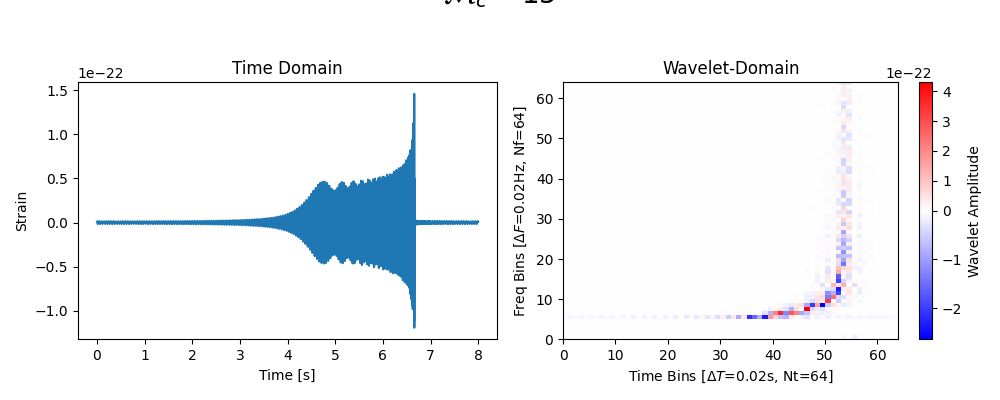
\includegraphics[width=\linewidth]{figures/cbc_imrphenom_d/cbc_wavelet_mc_15.png}
    \caption{$\mathcal{M}_c=15\ M_{\odot}$}
  \end{subfigure}

  \begin{subfigure}{0.5\textwidth}
    \centering
    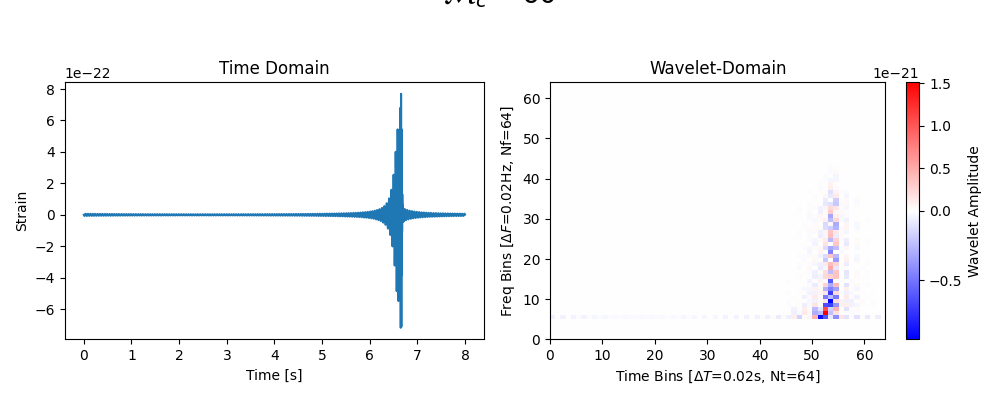
\includegraphics[width=\linewidth]{figures/cbc_imrphenom_d/cbc_wavelet_mc_60.png}
    \caption{$\mathcal{M}_c=60\ M_{\odot}$}
  \end{subfigure}

  \caption{Two CBC GW signals in time and wavelet domain. \avi{This plots' wavelet time and freq are bins: what time and frequencies do the bins correspond to?} \href{https://github.com/avivajpeyi/pywavelet/blob/main/docs/demos/cbc_demo.ipynb}{Link to code}.}
\end{figure}


\begin{figure}
  \centering

  \begin{subfigure}{0.5\textwidth}
    \centering
    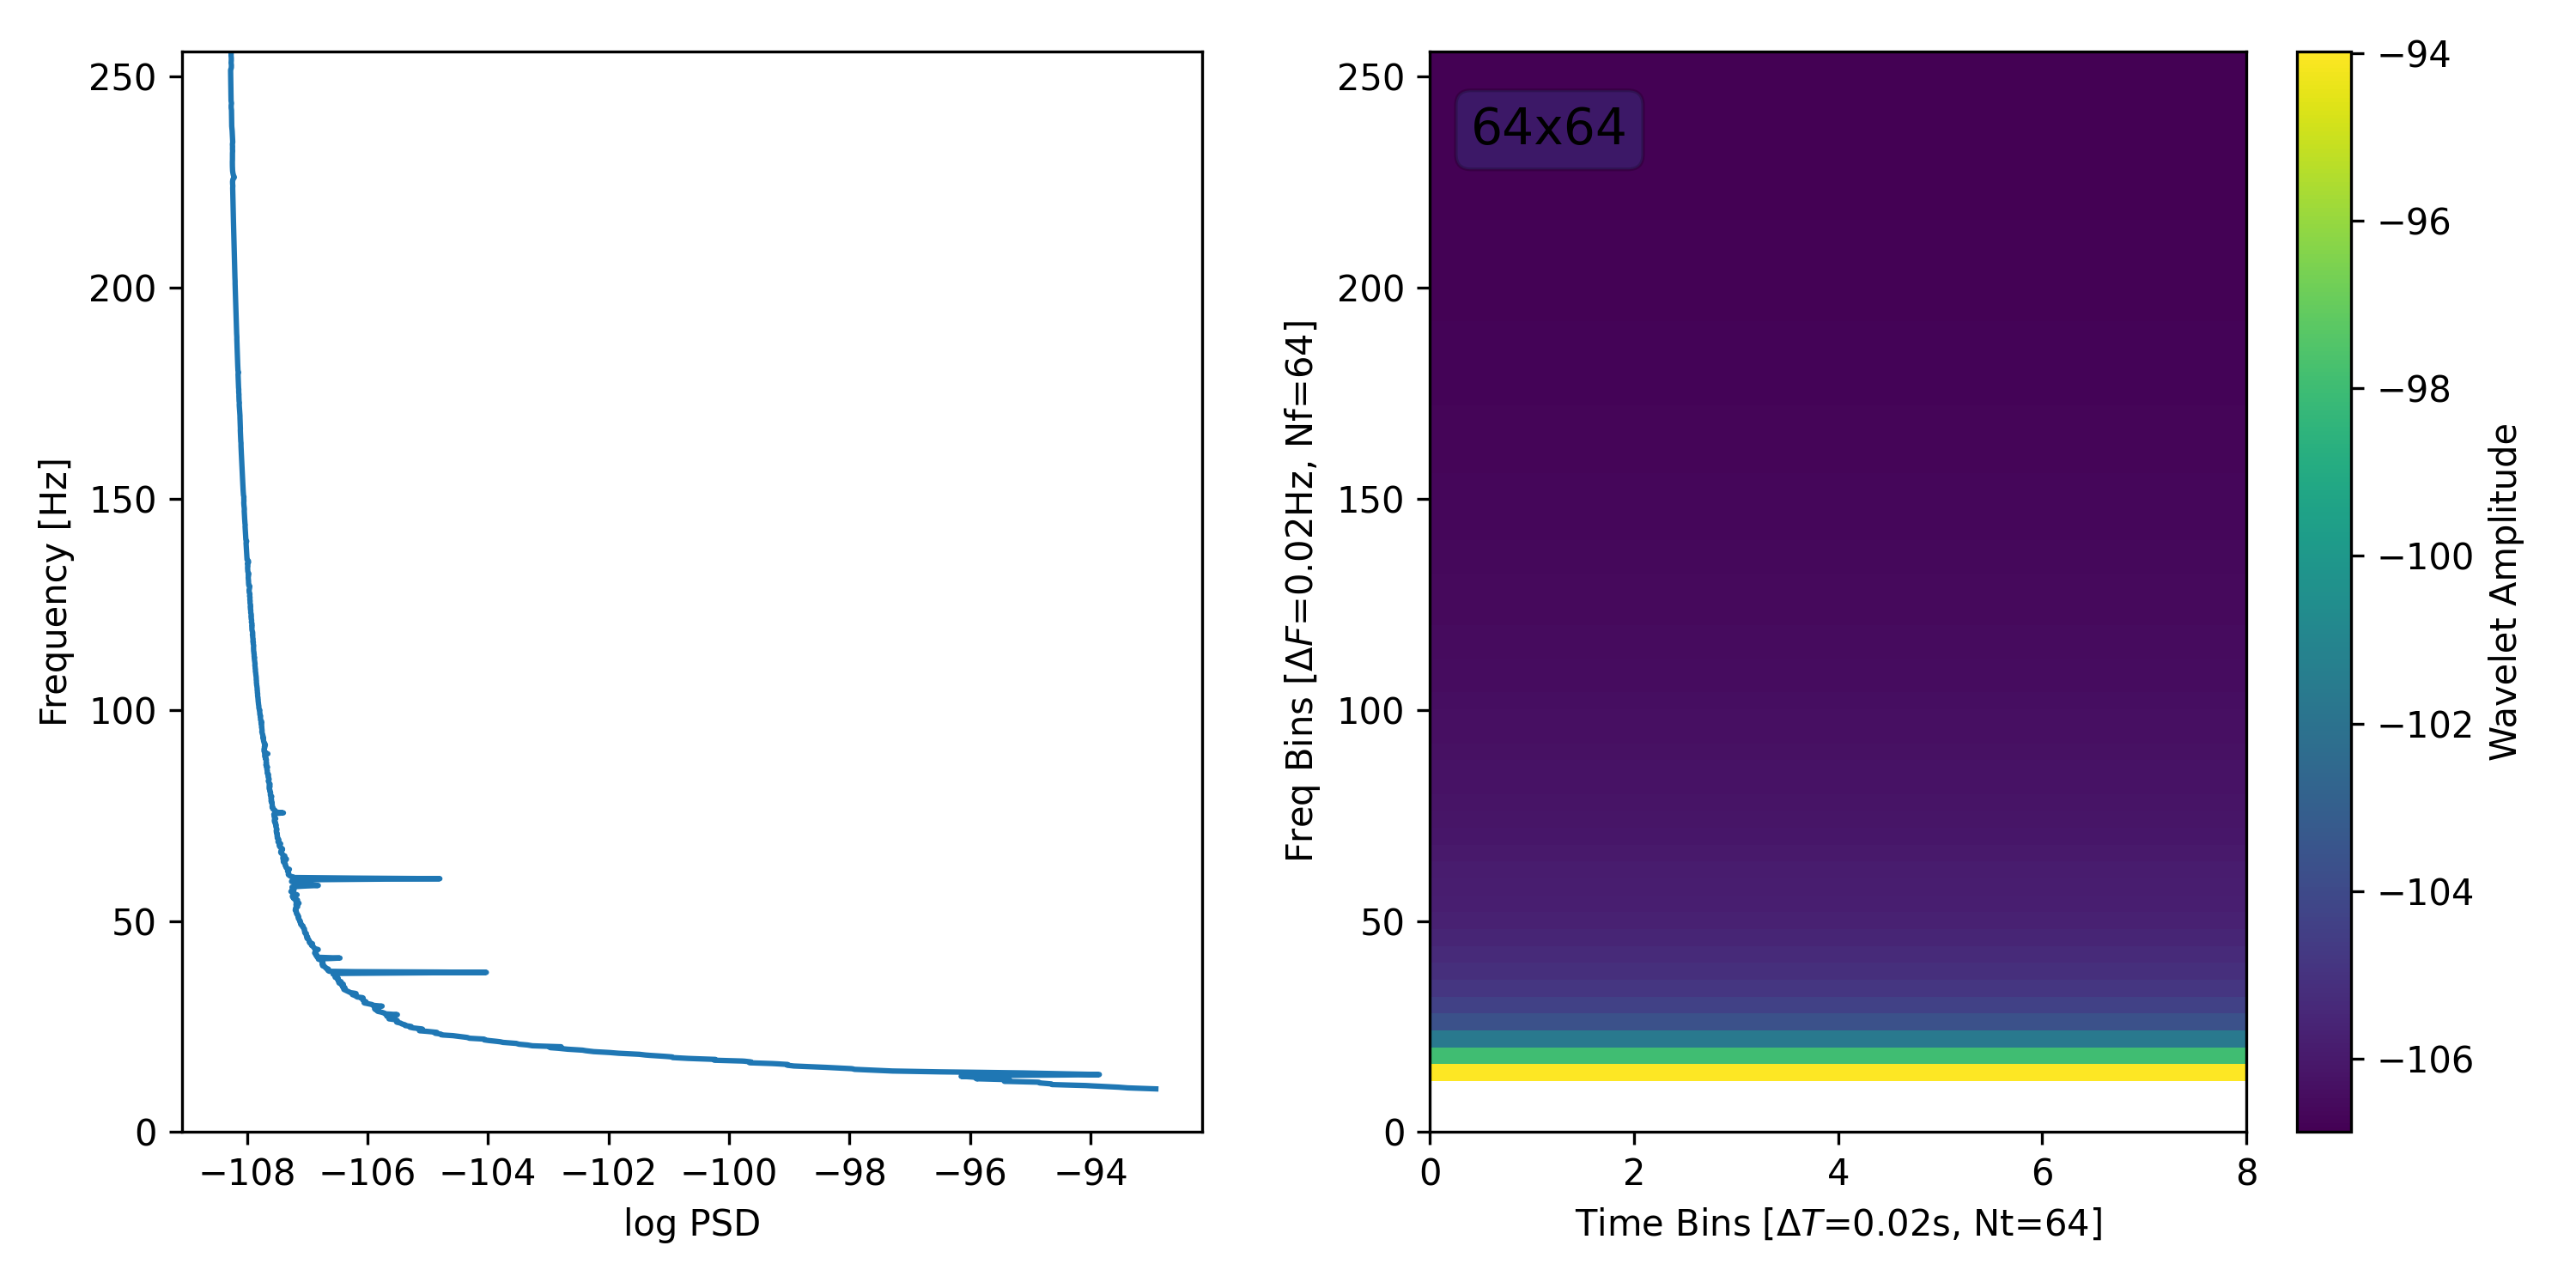
\includegraphics[width=\linewidth]{figures/PSD/psd_wavelet_64.png}
    \caption{$N_f=64$}
  \end{subfigure}

  \begin{subfigure}{0.5\textwidth}
    \centering
    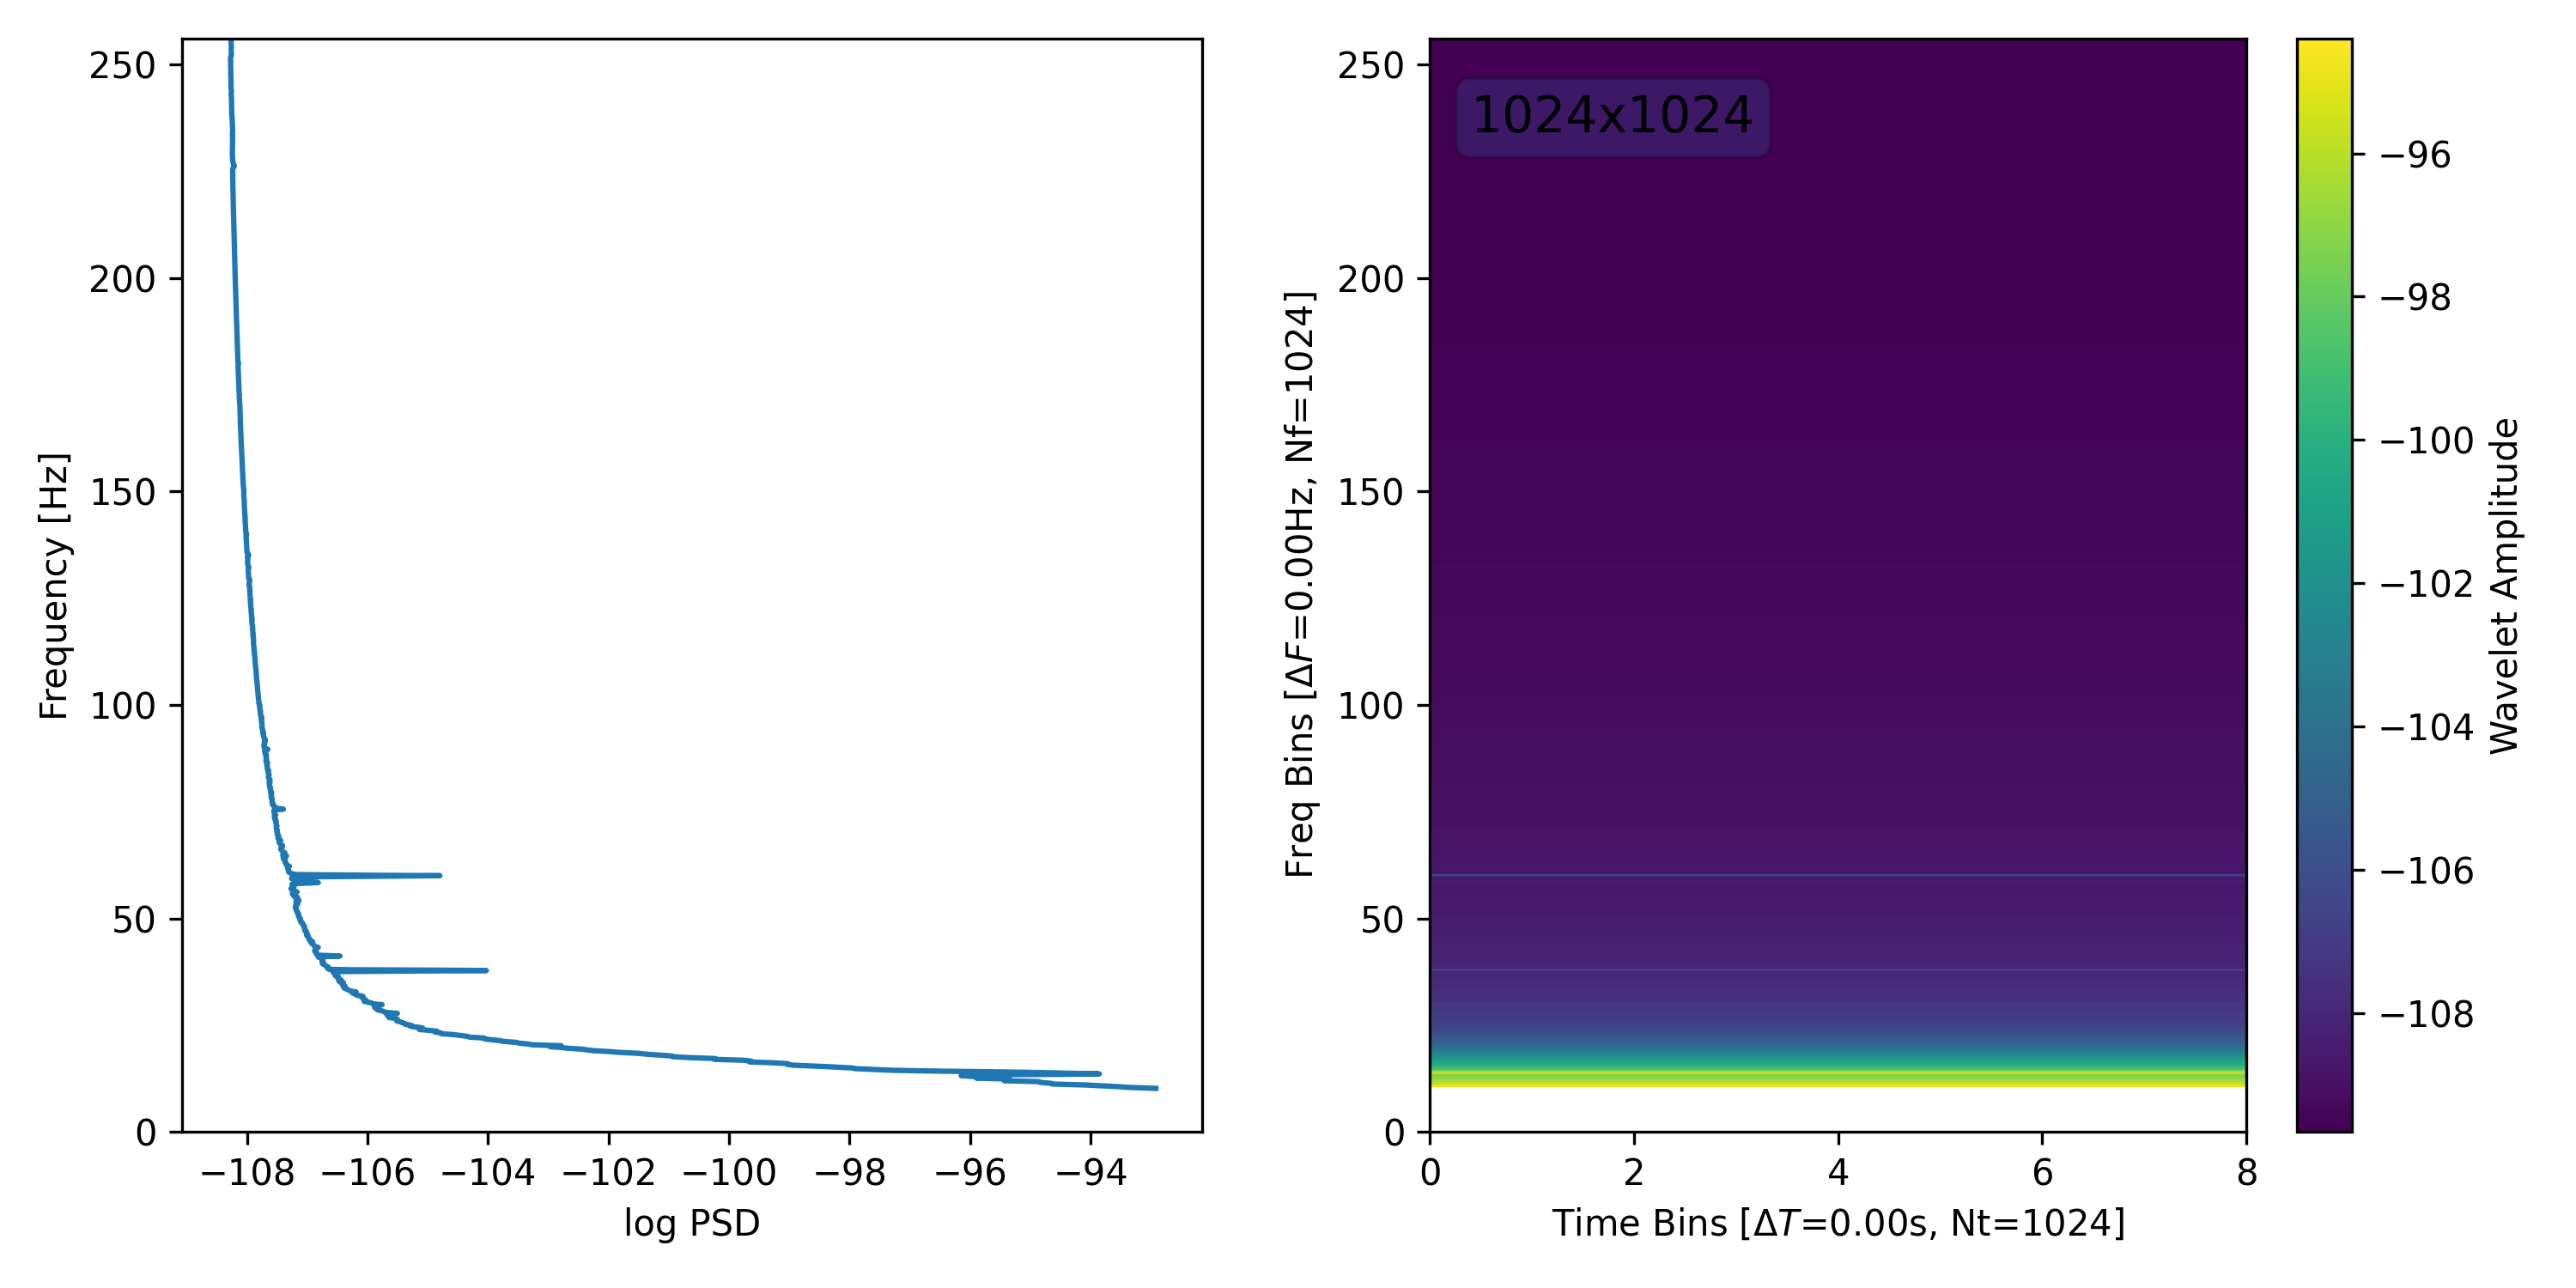
\includegraphics[width=\linewidth]{figures/PSD/psd_wavelet_1024.png}
    \caption{$N_f=1024$}
  \end{subfigure}

  \caption{Example of an evolutionary PSD generated from a stationary PSD using and different bin sizes. Note that some violin modes ($f\sim32, 64$ Hz) are not visible when using $N_f=64$ bins. \href{https://github.com/avivajpeyi/pywavelet/blob/main/tests/test_psd.py}{Link to code}.}
\end{figure}

\newpage
\section{PSD in wavelet domain [Giorgio]}
It took me a while to get familiar with the definitions of PSD, strain, etc, so I write it there for reference. A good reference in my opinion is \url{https://arxiv.org/abs/1408.0740}.
Let's consider ground-based instruments for simplicity since the generalization to the space-based ones is almost straightforward. In the \textbf{time} domain, each interferometer has a data stream
\begin{align}
s(t)&=h(t)+n(t)\nonumber\\
h(t)&=h_{ab}(t,\vec x)d^{ab}
\end{align}
where $h_{ab}(t,\vec x)$ is the time-dependent GW tensor, and $d^{ab}$ is the arm tensor.
The PSD lives in the time domain, therefore we introduce the Fourier-transformed data stream
\begin{align}
\tilde s(f)=\int_0^Tdt' s(t)\,e^{2\pi i f t'}\equiv \tilde h(f)+\tilde n(f)
\end{align}
with T the \textbf{total} observation time. And the PSD of the noise $S(f)$ is defined through the equation
\begin{align}\label{PSD_def_cont}
\langle \tilde n(f)\tilde n^*(f')\rangle=\frac 1 2 \delta(f-f')S(f)
\end{align}
where angle brackets $\langle\cdot\rangle$ denote an ensemble average over many noise realisations\footnote{We can assume ergodicity, therefore this can be translated into the average of the many measurements during the duration of the experiment}. A couple of observations are necessary:
\begin{itemize}
    \item $s(t)$ is adimensional, $\tilde s(f)$ has the dimension of a time
    \item $S(f)$ has the dimension of a time
    \item $S(f)$ is exactely the one plotted in \url{http://gwplotter.com/} as "Power Spectral Density". Please note it is plotted as a sqrt
\end{itemize}

\subsection{Simplified statistics of the wavelets}
We start from Eq.~\eqref{eq:direct}
\begin{equation}
w_{n m}=\sqrt{2} \Delta t \Re \left[C_{n m} \sum_{k=-K / 2}^{K / 2-1} e^{2\pi i k m q / K} x\left[n N_f+k\right] \phi[k]\right].
\end{equation}
where $K = 2q N_f$ is the width of the window function and $q$ determines the size of the window relative to the time resolution of the time-frequency pixels. We recall that we can approximate
\eqref{eq:wavelet_transform_continuous}
%
\begin{align}
w_{n m} &\approx \sqrt{2} \Re \left\{C_{n m} \int_{-\infty}^{+\infty} e^{2 \pi i t f_{m}} x(n \Delta T + t) \phi(t) dt\right\}=\nonumber\\
&=\sqrt{2} \Re \left\{C_{n m} \int_{-\infty}^{+\infty}dt\int_{-\infty}^{+\infty}df' e^{2 \pi i t (f_{m}-f)} e^{-2 \pi i n\Delta T f} \tilde x(f) \phi(t)\right\}
\end{align}
%
with $f_{m} = m\frac{f_{max}}{N_f}=m\frac{N}{2\,T\,N_f}=\frac{m}{2\Delta T}$. Here we used $dt=\Delta t$ to go to the continuous limit. Let's forget of the $\Re$ operator so far and let's compute the wavelet statistics for the noise $\tilde n(f)$, making use of \eqref{PSD_def_cont},
%
\begin{align}
\langle w_{n m}w_{n'm'}\rangle&\simeq C_{n m}C_{n'm'}\int dt\phi(t) \int dt' \phi(t')\int df e^{2 \pi i t (f_{m}-f)} e^{-2 \pi i (n-n')\Delta T f} e^{2 \pi i t' (f_{m'}-f)} S(f)\simeq\nonumber\\
&\simeq C_{n m}C_{nm'}\int dt\phi(t) \int dt' \phi(t')\int df e^{2 \pi i t (f_{m}-f)} e^{2 \pi i t' (f_{m'}-f)} S(f)
\end{align}
%
where we used the fact that $f\Delta T\gg 1$, enforcing $n=n'$. Now we can see immediately the Fourier transforms of the filters $\phi(t)$ and $\phi(t')$ and therefore write
%
\begin{align}
\langle w_{n m}w_{n'm'}\rangle\simeq C_{n m}C_{nm'}\int df S(f) \tilde\phi(f_{m}-f) \tilde\phi(f_{m'}-f)
\end{align}
%
Given that the two window functions have a limited support in frequency, a good approximation will be
%
\begin{align}
\langle w_{n m}w_{n'm'}\rangle&\simeq C_{n m}^2\int df S(f) \tilde\phi(f_{m}-f)^2\nonumber\\
&\simeq\delta_{nn'}\delta_{mm'} \Delta T S(f_{m})
\end{align}
%



\section{A simple GW chirp example}
The two polarizations ($+$ and $\cross$) for a chirping waveform in the quasi-circular-orbit limit are, for $t<t_{coal}$,
\begin{align}\label{eq:h_plus_cross}
h_+(t)&=\frac{1}{r}\left(\frac{GM_c}{c^2}\right)^{\frac{5}{4}}\left(\frac{5}{c\tau}\right)^{\frac{1}{4}}\frac{1+\cos^2\iota}{2}\cos(\phi(\tau))\nonumber\\
h_{\cross}(t)&=\frac{1}{r}\left(\frac{GM_c}{c^2}\right)^{\frac{5}{4}}\left(\frac{5}{c\tau}\right)^{\frac{1}{4}}\cos\iota\sin(\phi(\tau))
\end{align}
%
with
%
\begin{align}
\phi(\tau)&=-2\left(\frac{c^3\tau}{5GM_c}\right)^{\frac 5 8}+\phi_0\nonumber\\
\tau&=t_{coal}-t
\end{align}
and where $\phi_0$ is a time phase of the orbit, $M_c$ is the chirp mass of the binary, $r$ the distance of the source, $t_{coal}$ the time of coalescence and $\iota$ the inclination angle of the plane of the binary with respect to our line of sight. $G$ is the gravitational constant and $c$ the speed of light. For LIGO, which lives in the short-arm limit, the projected signal will be
%
\begin{align}\label{eq:proj_signal}
s(t)=\left(e^+_{ab}(\hat n)h^+(t) + e^{\cross}_{ab}(\hat n)h^{\cross}(t)\right)d^{ab}(t)
\end{align}
%
with $e_{ab}^{+/\cross}(\hat n)$ the polarization tensors, $\hat n$ the sky location of the binary and
%
\begin{align}
d^{ab}(t)=\frac{1}{2}\left(\hat u^a(t)\hat u^b(t)-\hat v^a(t)\hat v^b(t)\right)
\end{align}
%
with $\hat u(t)$ and $\hat v(t)$ the unit vectors of the two arm directions of the instrument.

\subsection{In the wavelet domain}
We write firstly the polarizations $h_+(t)$ and $h_{\cross}(t)$ \eqref{eq:h_plus_cross} in the wavelet domain making use of \eqref{eq:wavelet_time_approx_first_order}, obtaining
%
\begin{align}
A^+(t)&=\frac{1}{r}\left(\frac{GM_c}{c^2}\right)^{\frac{5}{4}}\left(\frac{5}{c(t_{coal}-t)}\right)^{\frac{1}{4}}\frac{1+\cos^2\iota}{2}\nonumber\\
A^{\cross}(t)&=\frac{1}{r}\left(\frac{GM_c}{c^2}\right)^{\frac{5}{4}}\left(\frac{5}{c(t_{coal}-t)}\right)^{\frac{1}{4}}\cos\iota\nonumber\\
\Psi^+(t)&=-2\left(\frac{c^3 (t_{coal}-t)}{5GM_c}\right)^{\frac 5 8}+\phi_0\nonumber\\
\Psi^{\cross}(t)&=-2\left(\frac{c^3 (t_{coal}-t)}{5GM_c}\right)^{\frac 5 8}+\phi_0+\frac{\pi}{2}\nonumber\\
\nu(t)&=\frac{5}{8\pi}\left(\frac{c^3}{5GM_c}\right)^{\frac 5 8}(t_{coal}-t)^{-\frac 3 8}
\end{align}
%
and the expression in terms of the wavelet coefficients will be
%
\begin{align}
\label{eq:wavelet_chirp}
w_{n m}^{+} &\approx \sqrt{2} \Delta t \Re C_{n m} \frac{1}{2} \frac{1}{r}\left(\frac{GM_c}{c^2}\right)^{\frac{5}{4}}\left(\frac{5}{c(t_{coal}-t_n)}\right)^{\frac{1}{4}}\frac{1+\cos^2\iota}{2}  \times\nonumber\\
&\times e^{-2i\left(\frac{c^3 (t_{coal}-n\Delta T)}{5GM_c}\right)^{\frac 5 8}+i\phi_0}\tilde{\phi}\left( f_{mq} -\frac{5}{8\pi}\left(\frac{c^3}{5GM_c}\right)^{\frac 5 8}(t_{coal}-t_n)^{-\frac 3 8} \right)\nonumber\\
w_{n m}^{\cross} &\approx \sqrt{2} \Delta t \Re C_{n m} \frac{1}{2} \frac{1}{r}\left(\frac{GM_c}{c^2}\right)^{\frac{5}{4}}\left(\frac{5}{c(t_{coal}-t_n)}\right)^{\frac{1}{4}}\cos\iota  \times\nonumber\\
&\times e^{-2i\left(\frac{c^3 (t_{coal}-n\Delta T)}{5GM_c}\right)^{\frac 5 8}+i\phi_0+i\frac{\pi}{2}}\tilde{\phi}\left( f_{mq} -\frac{5}{8\pi}\left(\frac{c^3}{5GM_c}\right)^{\frac 5 8}(t_{coal}-t_n)^{-\frac 3 8} \right)
\end{align}
%
It is easy to spot that, due to the fact that the arm directions change slowly with time, the signal of \eqref{eq:proj_signal} in wavelet domain will be
%
\begin{align}
w_{nm}^s=\left(e^+_{ab}(\hat n)w_{nm}^+ + e^{\cross}_{ab}(\hat n)w_{nm}^{\cross}\right)d^{ab}(t_n)
\end{align}




\bibliography{bibliography}%
\end{document}